\documentclass[a4paper,11pt]{article}
\usepackage[symbol]{footmisc}
\usepackage[hidelinks]{hyperref}
\hypersetup{
	colorlinks,
	linkcolor={blue!40!black},
	citecolor={blue!40!black},
	urlcolor={blue!40!black}
}
\renewcommand{\thefootnote}{\fnsymbol{footnote}}
\providecommand{\keywords}[1]{\textbf{\textit{Index terms---}} #1}

\usepackage{xcolor}
\usepackage[]{dmhdr} %dmanousakas style file for nice math defns
\usepackage{natbib}

\bibliographystyle{abbrv}

\begin{document}
\title{\bcores: Robust Large-Scale Bayesian Data Summarization in the Presence of Outliers}
\author{\stepcounter{footnote}Dionysis Manousakas$^{1,}$\thanks{Corresponding e-mail: \href{mailto:dm754@cam.ac.uk}{dm754@cam.ac.uk}} \and Cecilia Mascolo$^{1,2}$}
\date{%
		$^1$University of Cambridge\\%
		$^2$The Alan Turing Institute\\[2ex]%
}
\maketitle
% ************************** Thesis Abstract *****************************
% Use `abstract' as an option in the document class to print only the titlepage and the abstract.
\begin{abstract}
	\label{sec:abstract} 
	The proliferation of large-scale datasets offers unprecedented amounts of information for building trully intelligent machines, but at the same time poses a remarkable computational challenge: how can we efficiently process massive data? This thesis presents a suite of data reduction algorithms that enable scalable learning on large datasets, via extracting a succinct model-specific representation that summarizes the full data---a \emph{coreset}. Our frameworks support by design datasets of arbitrary dimensionality, and can be used for general purpose Bayesian inference under real-world constraints, including privacy preservation and robustness to outliers, encompassing diverse uncertainty-aware data analysis tasks, such as density estimation, classification and regression.
	%abundance, gathering, acquisition
   
    We motivate the necessity for novel data reduction techniques in the first place by developing a reidentification attack on coarsened representations of private behavioural data. Analysing longitudinal records of human mobility, we detect privacy-revealing structural patterns, that remain preserved in reduced graph representations of individuals information with manageable size. These unique patterns enable linkage attacks on individuals information via structural similarity computations on longitudinal mobility traces, revealing an existing privacy threat.
    
    We then propose a sparse variational inference scheme for approximating posteriors on large datasets via learnable weighted pseudodata, termed pseudocoresets. We show that the use of pseudodata enables overcoming the constraints on minimum summary size for given approximation quality, that are imposed on all existing Bayesian coreset constructions due to data dimensionality. Moreover, it allows us develop a scheme for pseudocoresets-based summarization that satisfies the standard framework of differential privacy by construction; in this way, we can release reduced size privacy-preserving representations for sensitive datasets that are amenable to arbitrary post-processing.
    
    Subsequently, we consider summarizations for large-scale Bayesian inference in scenarios when observed datapoints depart from the  statistical assumptions of our model. Using robust divergences, we develop a method for constructing cleansed coresets, which is able to automatically remove outliers from the generated data summaries. Thus we deliver robustified scalable representations for inference, that are suitable for applications involving contaminated and unreliable data sources.
    
    We demonstrate the performance of proposed summarization techniques on multiple parametric statistical models, and diverse simulated and real-world datasets, from music genre features to hospital readmission records, considering a wide range of data dimensionalities.%, from 2 to 500.
\end{abstract}

\keywords{Scalable learning; Big data summarizations; Coresets; Variational inference; Robust statistics; Noisy observations; Data valuation}
\section{Introduction}
\label{sec:introduction}

Machine learning systems perpetually collect growing datasets, such as product reviews, posting activity on social media, users feedback on services, or insurance claims. The rich information content of such datasets has opened up an exciting potential to remedy various practical problems. Hence, recent years have witnessed a surge of interest in scaling up inference in the large-data regime via stochastic and batch methods~\cite{angelino16, hoffman13, welling11}. Most of related approaches have treated datapoints indiscriminantly; nevertheless, it is well known that not all datapoints contribute equally valuable information for a given target task~\cite{ghorbani19}. 

Datasets collected in modern applications contain redundant input samples that reflect very similar statistical patterns, or multiple copies of identical observations. Often input aggregates subpopulations emanating from different distributions~\cite{zheng08, zhuang15}. Moreover, the presence of outliers is a ubiquitous challenge, attributed to multiple causes. In the first place, noise is inherent in most real-world data collection procedures, creating systematic outliers: crowdsourcing is prone to mislabeling~\cite{frenay13} and necessitates laborious data cleansing~\cite{lewis04, paschou10}, while measurements commonly capture sensing errors and system failures. Secondly, outliers can be generated intentionally from information contributing parties, who aim to compromise the functionality of the application through data poisoning attacks~\cite{barreno10, biggio12, li16, koh17, steinhardt17, ghorbani19}, realised for example via data generation from fake accounts. Outliers detection is  challenging, particularly in high dimensions~\cite{lucic16outliers, diakonikolas19, dickens20}. Proposed solutions \mbox{often are} model-specific, and include dedicated learning components which increase the time complexity of the application, involve extensive hyperparameter tuning, introduce data redundancies, or require model retraining~\cite{sheng08, whitehill09, raykar10, karger11, liu12, zhang16}. On the other hand, operating on a corrupted dataset is brittle, and can decisively degrade the predictive performance of downstream statistical tasks, deceptively underestimate model uncertainty and lead to incorrect decisions. 

In this work, we design an integrated approach for inference on massive scale observations that can jointly address scalability and data cleansing for complex Bayesian models, via robust data summarization. Our method inherits the full set of benefits of Bayesian inference and works for any model with tractable likelihood function. At the same time, it maintains a high degree of automation with no need for manual data inspection, no additional computational overhead due to robustification, and can tolerate a non-constant number of corruptions. Moreover, our work points to a more efficient practice in large-scale data acquisition, filtering away less valuable samples, and indicating the regions of the data space that are most beneficial for our inference task. 

Our solution can be regarded as an extension of Bayesian coreset methods that can encompass robustified inference. Bayesian coresets~\cite{huggins16, campbell19jmlr, campbell19neurips} have been recently proposed as a method that enables Bayesian learning at scale via substituting the complete dataset over inference with an informative sparse subset thereof. Robustified Bayesian inference methods~\cite{berger94} have sought solutions to mismatches between available observations and the assumed data generating model, %via generalizing the data likelihood function, 
via proposing heavy-tailed data likelihood functions~\cite{huber09, insua12} and localization~\cite{definetti61, wang18}, using robust statistical divergences~\cite{futami18, knoblauch18, miller19},  or inferring datapoints-specific importance weights~\cite{wang17}. Here, we cast coreset construction in the framework of robustified inference, introducing \emph{\bcores{}}, a method that learns sparse variational approximations of the full data posterior under the \bdiv{}. In this way, we are able to yield summaries of large data that are distilled from outliers, or data subpopulations departing from our statistical model assumptions. Importantly, \bcores{} can act as a preprocessing step, and the learned data summaries can subsequently be given as input to any ordinary or robustified black-box inference algorithm.

The rest of this chapter is organized as follows. In \cref{sec:preliminaries,sec:method} we introduce necessary concepts from Bayesian inference, and present our proposed method. In \cref{sec:evaluation} we expose experimental results on simulated and real-world benchmark datasets: we consider diverse statistical models and scenarios of extensive data contamination, and demonstrate that, in contrast to existing summarization algorithms, our method is able to maintain reliable predictive performance in the presence of structured and unstructured outliers. Finally, in \cref{sec:conclusion} we provide conclusions and discuss future works.

This chapter is based on~\citep{beta-cores}.





%\section{Preliminaries}
\label{sec:preliminaries}

In this section, we introduce the required concepts from Bayesian inference, present robustness limitations of standard posterior on big data, and outline existing generalizations of the posterior that aim to robustify inference with respect to data mismatch.

\subsection{Standard Bayesian inference and lack of robustness in the large-data regime}
In the context of Bayesian inference, we are interested in updating our beliefs about a vector of random variables $\theta \in \Theta$, initially expressed through a prior distribution $\pi_0(\theta)$, after observing a set of datapoints $ x:=(x_n)_{n=1}^{N} \in \mcX^N$.  Posterior on $\theta$ can be computed via the application of Bayes rule 
\[
\pi(\theta|x) = \frac{1}{Z'}\pi(x|\theta)\pi_0(\theta),
\label{eq:bayes-rule}
\] 
where $Z'$ is a (typically intractable) normalization constant, and $\pi(x|\theta)$ is the likelihood of our observations according to an assumed statistical model.
When datapoints are conditionally independent given $\theta$---which is the primary focus of this work---likelihood gets factorized as $\pi(x|\theta) = \Pi_{n=1}^{N}\pi(x_n|\theta)$. An equivalent formulation of  the
Bayesian posterior as a solution to an optimization problem was proposed by Zellner~\citep{zellner88}, which is written as  
\[
\pi(\theta|x) = \frac{1}{Z'} \exp\left(-\xent{\hpi(x)}{\pi(x|\theta)}\right)\pi_0(\theta).
\label{eq:zellner-rule}
\]
In the above, $\hpi(x)$ is the empirical distribution of the observed datapoints. The exponent $\xent{\hpi(x)}{\pi(x|\theta)}:=-\sum_{n=1}^{N}\log\pi(x_n|\theta)$
corresponds (up to a constant) to the \emph{cross-entropy}, which is  equal to the empirical average of negative log-likelihoods of the datapoints, and quantifies the expected loss incurred by our estimates for the model parameters $\theta$ over the available observations, under the \emph{Kullback-Leibler~(KL) divergence}.

When $N$ is large, the Bayesian posterior is strongly affected by perturbations in the observed data space. To develop an intuition on this, assuming that the true and observed data distributions have densities $\pi_\theta$ and $\pi_\textsubscript{obs}$ respectively, we can rewrite an approximation of~\cref{eq:zellner-rule} via the KL divergence ($\plainkl$) as~\cite{miller19}
\[
\pi(\theta|x) 
& \propto  \exp\left(\sum_{n=1}^{N}\log\pi(x_n|\theta)\right) \pi_0(\theta)
\doteq	 \exp\left(N \int \pi_\textsubscript{obs} \log \pi_\theta\right) \pi_0(\theta) \\
 &:= \exp\left(-N \kl{\pi_\textsubscript{obs}}{\pi_\theta}\right) \pi_0(\theta),
 \label{eq:missmatch_with_N}
\]
where $\doteq$ denotes  agreement to first order in exponent.\footnote{i.e. $a_n \doteq b_n$ iff $(1/n)\log(a_n/b_n) \rightarrow 0$}
Hence, due to the large $N$ in the exponent, small changes to $\pi_\textsubscript{obs}$ will have a large impact on the posterior.

\subsection{Robustified posteriors}

Robust inference methods aim to adapt~\cref{eq:bayes-rule} to formulations that can address the case of observations departing from model assumptions, as often happening in practice, e.g. due to misspecified shapes of data distributions and number of components, or due to the presence of outliers. In such formulations~\citep{dawid16, jewson18, fujisawa08, eguchi01}, Bayesian updates rely on utilising robust divergences instead of the KL divergence, to express the losses over the data. 

A popular choice~\citep{futami18, knoblauch18} for enhancing robustness of inference is replacing the log-likelihood terms arising in~\cref{eq:zellner-rule} with the \emph{\bdiv~}(or \emph{density power divergence})~\citep{basu98, cichocki10}, which yields the following posterior for $\theta$~\citep{ghosh16,knoblauch18}
\[
\pi_\beta(\theta|x) \propto \exp\left(-\db{\hpi(x)}{\pi(x|\theta)}\right)\pi_0(\theta),
\label{eq:b-posterior}
\] 
where 
\[
\db{\hpi(x)}{\pi(x|\theta)} := 
 -\sum_{n=1}^{N}  \underbrace{\left(\frac{\beta+1}{\beta}\pi(x_n|\theta)^{\beta} + \int_{\mcX} \pi(\chi|\theta)^{1+\beta}d\chi\right)}_{:=f_n(\theta)},
\label{eq:b-loss}
\]
with $\beta>0$.
We refer to quantities defined in~\cref{eq:b-posterior,eq:b-loss} as the \emph{\bpost{}} and \emph{\blik{}} respectively. Noticeably, the individual terms $f_n(\theta)$  of the \blik{} %, which are known as the Tsallis scores~\citep{tsallis88}, are decomposed into a data-independent $c(\theta)$, and a data-dependent part $t_n(\theta)$.
% := \frac{1}{\beta} \pi(x_n|\theta)^{\beta}$. 
%The latter 
allow attributing \emph{different strength of influence to each of the datapoints}, depending on their accordance with the model assumptions. As densities get raised to a suitable power $\beta$, outlying observations are exponentially downweighted. When $\beta \rightarrow 0$,~\cref{eq:zellner-rule} is recovered and all datapoints are treated equally.

In the presentation above we focused on modeling observations $(x_n)_{n=1}^{N}$~(unsupervised learning). In the case of supervised learning on data pairs ${(x_n,y_n)}_{n=1}^{N} \in (\mcX \times \mcY)^N$, the respective expression for individual terms of \blik{}\footnote{In this context for simplicity we use notation $f_n(\cdot)$  to denote $f(y_n|x_n, \cdot)$.} is~\cite{basu98}
\[
f_n(\theta):= -\frac{\beta+1}{\beta}\pi(y_n|x_n,\theta)^{\beta} +  \int_{\mcY} \pi(\psi|x_n,\theta)^{1+\beta}d\psi.
\label{eq:sl-lik-terms}
\] 
\section{Method}
\label{sec:method}

In this section we discuss \bcores, our unified solution to the robustness and scalability challenges of large-scale Bayesian inference. \cref{subsec:sparse-b-posterior} introduces the main quantity of interest in our inference method, and shows how it addresses the exposed issues. \cref{subsec:bb-construct} presents an iterative algorithm that allows efficient approximate computations of our posterior.


\subsection{Sparse \bpost{}}
\label{subsec:sparse-b-posterior}


Scaling up the computation of the robust $\beta$-posterior~\cref{eq:b-posterior} in the regime of massive datasets for non-conjugate models is challenging:
%~Closed form computation of~\bdiv{} is not possible for a large number of statistical models. Moreover, 
similarly to the standard Bayesian posterior~\cref{eq:bayes-rule}, applying Markov chain Monte Carlo~(MCMC) methods to sample from the~\bpost{}, implies a computational cost scaling at order $\Theta(N)$. 

Bayesian coresets~\cite{huggins16,campbell19jmlr} have been recently proposed as a method to circumvent the computational cost for the purposes of approximate inference via summarizing the original dataset  $(x_n)_{n=1}^{N}$ with a small learnable subset of weighted datapoints $(x_m, w_m)_{m=1}^{M}$, where  $(w_m)_{m=1}^{M} \in \reals^{M}_{+},\; M \ll N$. 
Substituting~\cref{eq:b-loss} in ~\cref{eq:b-posterior}, allows us to explicitly introduce a weights vector $ w \in \reals_{\geq 0}^{N}$ in the posterior, and rewrite the latter in the general form
\[
\pi_{\beta,w}(\theta|x) 
= \frac{1}{Z(\beta, w)}  \exp\left(\sum_{n=1}^{N}w_nf_n(\theta)\right)\pi_0(\theta).
\label{eq:bcore-posterior}
\]
%In the last line the data-independent part of the Tsallis score has been absorbed in the uknown log-partition function of the distribution.
In the case of the \bpost{} on the full dataset~\cref{eq:b-posterior}, we have $w=\vecone \in\reals^{N}$; for coreset posteriors this vector acts as a learnable parameter and attains a non-trivial sparse value, with non-zero entries corresponding to the elements of the full dataset that are selected over the summarization.

Although Bayesian coresets can dramatically reduce inference time, they inherit the susceptibility of Bayesian posterior to data mismatch in the large data regime: even though the number of points used in inference gets reduced, these points are now weighted, hence the remark of~\cref{eq:missmatch_with_N} can carry over in coresets posterior. 

The recent formulation of Riemannian coresets~\citep{campbell19neurips} has framed the problem of coreset construction as Variational Inference~(VI) in a sparse exponential family. Our method provides a natural extension of this framework to robust divergences. Here we aim to approximate data posterior via a \emph{sparse \bpost}, which can be expressed as follows
\[
w^{*} = \arg \min_{w\in\reals^{N}} \kl{\pi_{\beta,w}}{\pi_{\beta}} 
\quad
\text{s.t.}
\quad
w \geq 0,\; ||w||_0 \leq M,
\label{eq:coreset-vi}
\]
%where $\plainkl$ is the KL divergence. 
In the following we denote expectations and covariances under $\theta \sim \pi_{\beta,w}(\theta|x)$ as $\EE_{\beta,w}$ and $\cov_{\beta,w}$ respectively. Then the KL divergence is written as
\[
\kl{\pi_{\beta,w}}{\pi_{\beta}}:=\EE_{\beta, w} \left[\log\frac{\pi_{\beta,w}}{\pi_\beta}\right].
\label{eq:kld}
\]
In our formulation it is easy to observe that posteriors of~\cref{eq:bcore-posterior} form a set of \emph{exponential family distributions}~\cite{wainwright08}, with natural parameters $w \in \reals_{\geq 0}^N$, sufficient statistics $(f_n(\theta))_{n=1}^{N}$, and log-partition function $\log Z(\beta, w)$. Following~\citep{campbell19neurips}, the objective can be expanded as 
\[
\kl{\pi_{\beta,w}}{\pi_{\beta}} =& \log Z(\beta) - \log Z(\beta, w) 
                                    - \sum_{n=1}^{N}\EE_{\beta,w}\left[f_n(\theta)- w_n f_n(\theta)\right],
\label{eq:sparsevi-obj}
\]
and minimized via gradient descent on %$\beta$ and 
$w$.  %As detailed in~\cref{sec:gradient-derivations}, 
The gradient of the objective of~\cref{eq:sparsevi-obj} can be derived in closed form, as  
\[
\nabla_{w}\kl{\pi_{\beta,w}}{\pi} 
												   & = -\cov_{\beta,w}\left[f,(1 -w)^Tf\right], 
\label{eq:dkl-grad}
\]
where $f:=\left[f_1(\theta) \ldots f_N(\theta)\right]^T$.%, $f':=\left[f'_1(\theta) \ldots f'_N(\theta)\right]^T$.




\subsection{Black-box stochastic scheme for incremental coreset construction}
\label{subsec:bb-construct}



\begin{algorithm*}[!t]
	\caption{Incremental construction of sparse \bpost{}}
	\label{alg:bcores}
	\begin{algorithmic}[1]
		\Procedure{\bcore}{$f,  \pi_0, x, M, B, S, T, (\gamma_t)_{t=1}^{\infty}$, $\beta$}
		\State $w \assign \mathbf{0} \in \reals^{M}$,\;\; $g \assign \mathbf{0} \in \reals^{S \times M}$, \;\;$g' \assign \mathbf{0} \in \reals^{S \times B}$, \;\;$\mcI \assign \emptyset$
		\For{$m =1, \ldots, M $}
		\LineCommentIndent{Take S samples from current coreset posterior}
		\State $(\theta)_{s=1}^{S}  \distiid \pi_{\beta,w} \propto \exp \left(w^Tf\right) \pi_0(\theta)$
		\LineComment{Obtain a minibatch of $B$ datapoints from the full dataset}
		\State $\mcB\dist\distUnifSubset\left([N], B\right)$
		\LineComment{Compute the \blik{} vectors over the coreset and minibatch datapoints for each sample}
		\State $g_{s} \gets \left( f(x_m, \theta_s, \beta ) - \frac{1}{S}\sum_{r=1}^S f(x_m, \theta_{r}, \beta) \right)_{m \in \mcI}\in \reals^M$ 
		\State  $g'_{s} \gets \left( f(x_b, \theta_s, \beta) - \frac{1}{S}\sum_{r=1}^S f(x_b, \theta_{r}, \beta) \right)_{b\in\mcB} \in \reals^B$
		\LineComment{Get empirical estimates of correlation over the coreset and minibatch datapoints}
		\State $\hcorr \assign \diag \left[ \frac{1}{S} \sum_{s=1}^{S} g_{s}
		{g_{s}}^T\right]^{-\frac{1}{2}} \left(\frac{1}{S} \sum_{s=1}^{S} g_{s} \left(\frac{N}{B}1^T g'_{s} - w^T g_{s}\right)\right) \in \reals^{M}$
		\label{lst:line:core-corr}
		\State $\hcorr' \assign \diag \left[ \frac{1}{S} \sum_{s=1}^{S} g'_{s}
		{g'_{s}}^T\right]^{-\frac{1}{2}} \left(\frac{1}{S} \sum_{s=1}^{S} g'_{s} \left(\frac{N}{B}1^T g'_{s} - w^T g_{s}\right)\right)  \in \reals^{B}$
		\label{lst:line:batch-corr}
		\LineComment{Add next datapoint via correlation maximization}
		\State $n^{\star} \assign \arg \underset{n \in [m] \cup [B]}{\max} \left( \left|\hcorr \right| \cdot \vecone[n \in \mcI] + \hcorr' \cdot \vecone [n \notin \mcI]\right)$, \;\;$ \mcI \assign \mcI \cup \{n^{\star}\}$
		\For{$ t = 1, \ldots, T$} 		\Commenttriangle{Optimize weights vector via projected gradient descent}
		\State $(\theta)_{s=1}^{S}  \distiid \pi_{\beta,w}(\theta) \propto \exp\left(w^T f\right)\pi_0(\theta)$ 
		\State $\mcB\dist\distUnifSubset\left([N], B\right)$
		\LineComment{Compute gradient terms discretizations over the coreset and minibatch datapoints for each sample}
		\For{$s = 1, \dots, S$} 
		\State $g_{s} \gets \left( f(x_m, \theta_s, \beta) - \frac{1}{S}\sum_{r=1}^S f(x_m, \theta_{r}, \beta) \right)_{m\in\mcI} \in \reals^M$  
		\State $g'_{s} \gets \left( f(x_b, \theta_s, \beta) - \frac{1}{S}\sum_{r=1}^S f(x_b, \theta_{r}, \beta) \right)_{b\in\mcB} \in \reals^B$  	
		\EndFor
		\LineComment{Compute MC gradients for variational parameters}
		\State $\hat\nabla_w \gets -\frac{1}{S}\sum_{s=1}^S g_s\left( \frac{N}{B} 1^Tg'_s- w^Tg_s\right)$
		%, $\hat\nabla_\beta \gets -w^T\frac{1}{S}\sum_{s=1}^S k_s\left( \frac{N}{B} 1^Tg'_s- w^Tg_s\right)$
		\label{lst:line:mc-grad}
		\LineComment{Take a projected stochastic gradient step}
		\State $w \gets \max(w - \gamma_t\hat\nabla_w, 0)$
		%, $\beta \gets \max(\beta - \gamma_t\hat\nabla_\beta, 0)$
		\EndFor
		\EndFor
		\State\Return $w$%, $\beta$
		\EndProcedure		 
	\end{algorithmic}
\end{algorithm*}


To scale up coreset construction on massive datasets we use stochastic gradient descent on minibatches $\mcB \sim \distUnifSubset([N], B)$, with $B \ll N$.
The covariance of~\cref{eq:dkl-grad} required for exact gradient computation of the variational objective is generally not available in analytical form. Hence, for our black-box coreset construction we approximate this quantity via Monte Carlo estimates, using samples of the unknown parameters from the coreset posterior. These samples can be efficiently obtained with complexity $O(M)$ (not scaling with dataset size $N$) due to the sparsity of the coreset posterior over the procedure. The proposed black-box construction makes no assumptions on the statistical model other than having tractable \blik{}s. We employ a two-step incremental scheme, with complexity of order $O\left(M(M+B)ST\right)$, where $S$ is the number of samples from the coreset posterior, and $T$ is the total number of iterations over coreset points weights optimization. The full incremental construction is outlined in \cref{alg:bcores}.


\subsubsection{Next datapoint selection}
We first select the next datapoint to include in our coreset summary, via a greedy selection criterion. Although maximizing decrease in KL locally via~\cref{eq:dkl-grad}, seems to be the natural greedy choice here, using the information-geometric argument presented in~\cite{campbell19neurips}, we use instead the following correlation maximization criterion:
\[
x_{m} = \arg \underset{x_m \in \mcI \cup \mcB }{\max}
\begin{cases}
	\left|\corr_{\beta,w}\left[f_m, \frac{N}{B}1^Tf - w^T f\right]\right| & w_m>0 \\
	\corr_{\beta,w}\left[f_m, \frac{N}{B}1^Tf - w^T f\right] & w_m=0,
\end{cases}
\label{eq:greedy-select}
\]
where we denoted by $\mcI$ the set of coreset points.
The correlations for coreset and minibatch datapoints are empirically approximated  as in lines~\ref{lst:line:core-corr} and~\ref{lst:line:batch-corr} of~\cref{alg:bcores} respectively.
\begin{comment}
\[
\hcorr = \diag \left[ \frac{1}{S} \sum_{s=1}^{S} g_s g_s^T \right]^{-\frac{1}{2}} \left(\frac{1}{S} \sum_{s=1}^{S} g_s \left(\frac{N}{B}1^Tg_s- w^Tg_s\right) \right),
\label{eq:empirical-corr}
\]
where 
 \[
 g_s:= \begin{bmatrix}
		f_1(\theta_s) \\
		\vdots \\
		f_N(\theta_s)
\end{bmatrix}
-
\frac{1}{S}\sum_{r=1}^{S}
 \begin{bmatrix}
f_1(\theta_r) \\
\vdots \\
f_N(\theta_r)
\end{bmatrix}.
\label{eq:sampled-potentials}
\]
\end{comment}

\subsubsection{Coreset points reweighting}
After adding a new datapoint we update the coreset weight vector $w\in\reals_{\geq 0}$ via $T$ steps of projected stochastic gradient descent, using the Monte Carlo estimate of~\cref{eq:dkl-grad} per line~\ref{lst:line:mc-grad} of~\cref{alg:bcores}.
\begin{comment}
\[
\hat{\nabla}_w := -\frac{1}{S} \sum_{s=1}^{S} g_s \left(\frac{N}{B}1^Tg_s - w^T g_s\right) \in \reals_{d}, 
\label{eq:gradw}
\]
where $g_s$ are defined as in~\cref{eq:sampled-potentials}.
\end{comment}
\vspace{.2cm}
\par 
\textbf{Summarization of observations groups and batches.}
Apart from working at the individual datapoints level, our scheme also enables summarizing batches and groups of observations. Acquiring efficiently informative batches of datapoints can replace random minibatch selection commonly used in stochastic optimization for large-scale model training. This extension can also be quite useful in situations where datapoints are partitioned in clusters, e.g. according to demographic information. For example, when gender and age features are available in datasets capturing users movies habits, collected datapoints can be binned accordingly, and our group summarization technique will allow extracting informative combinations of demographic groups that can jointly summarize the entire population's information. The robustness properties of \bcores{} in such applications can aid removing group bias, and rejecting groups with large fractions of outliers. \cref{alg:bcores} is again directly applicable, where $g_s$ vectors are now summed over the corresponding datapoints of each batch or group.

\section{Experiments \& applications}
\label{sec:evaluation}
\definecolor{darkblue}{rgb}{0.0, 0.0, 0.55}
\definecolor{oxfordblue}{rgb}{0.0, 0.13, 0.28}
\definecolor{mydarkblue}{rgb}{0,0.08,0.45}
\newcommand{\MYhref}[3][mydarkblue]{\href{#2}{\color{#1}{#3}}}%

We examine the inferential results achieved by our method under 3 statistical models, in scenarios capturing different types of data mismatch with reality. The data contamination models used in following experiments are reminiscent of \emph{Huber's $\eps$-contamination model}~\citep{huber92}, which postulates that observed data are generated from a mixture of distributions of the form $(1-\eps)\cdot G+ \eps\cdot Q$, where $\eps \in (0,1)$,  $G$ is a distribution of inliers captured by the assumed statistical model, and $Q$ is an arbitrary distribution of outliers. This model has found use in several recent studies on robust statistical estimators suitable for underlying data distributions with minimal assumptions~\citep{wei17, chen18}.

\bcores{} is compared against a uniformly random sampling baseline, and stochastic batch implementations of two existing Riemannian coreset methods: 
\benum[label={(\roman*)}]
	\item \sparsevi~\citep{campbell19neurips}, which builds up a coreset according to an incremental scheme similar to ours, considering the standard likelihood function terms evaluated on the dataset points, and 
	\item \psvi~\citep{psvi}, the method introduced in~\cref{chap:chap4}, which runs a batch optimization on a set of pseudopoints, and uses standard likelihood evaluations to jointly learn the pseudopoints' weights and locations, so that the extracted summary resembles the statistics of the full dataset. 
\eenum


We default the number of iterations in the optimization loop over gradient-based coreset constructions to $ T = 500$, using a learning rate $ \gamma_t \propto t^{-1}$ and $S=100$ random projections per gradient computation. For consistency with the compared baselines, we evaluate inference results obtained by \bcores{} using the classical Bayesian posterior from~\cref{eq:bayes-rule} conditioned on the corresponding robustified data summary. Additional details on used benchmark datasets are presented in~\cref{sec:data-details}. 

\subsection{Simulated Gaussian mean inference under stuctured data contamination}
\label{subsec:gauss-expt}

In the first experiment we study how \bcores{} behaves in the setting of mean inference on synthetic $d$-dimensional data, sampled \iid from a normal distribution with known covariance,
\[
\theta \sim \distNorm\left(\mu_0, \Sigma_0\right),
\qquad 
\;\;\;\;\;
x_n \distiid \distNorm(\theta, \Sigma),
\qquad
n = 1, \ldots, N.
\label{eq:mvn-expt}
\]
In the presented results, we use priors $\mu_0=\mathbf{0}$ and $\Sigma_0=I$,  dimensionality $d=20$ and dataset size $N=5,000$.
 
We consider the case of structured data contamination existing in the observations, simulated as follows: Observed datapoints are typically sampled from a Gaussian $ \distNorm(\mathbf{1}, I)$. At a percentage $F\%$,  data collection fails; in this case, datapoints are collected from a shifted Gaussian $ \distNorm(\mathbf{10}, I)$. Consequently, the observed dataset forms a Gaussian mixture with two components; however, our statistical model assumes only a single Gaussian.

\begin{figure}[!htp]
	\centering 
	\begin{subfigure}[ht]{0.96\textwidth} 
		\includegraphics[width=1.\textwidth]{\MyPath/figs/gauss_scatterplot.png}
		\caption{\label{fig:beta_gaussian_coreset_points}}
	\end{subfigure}
	\hfill\qquad
	\begin{subfigure}[ht]{0.96\textwidth} 
		\centering
		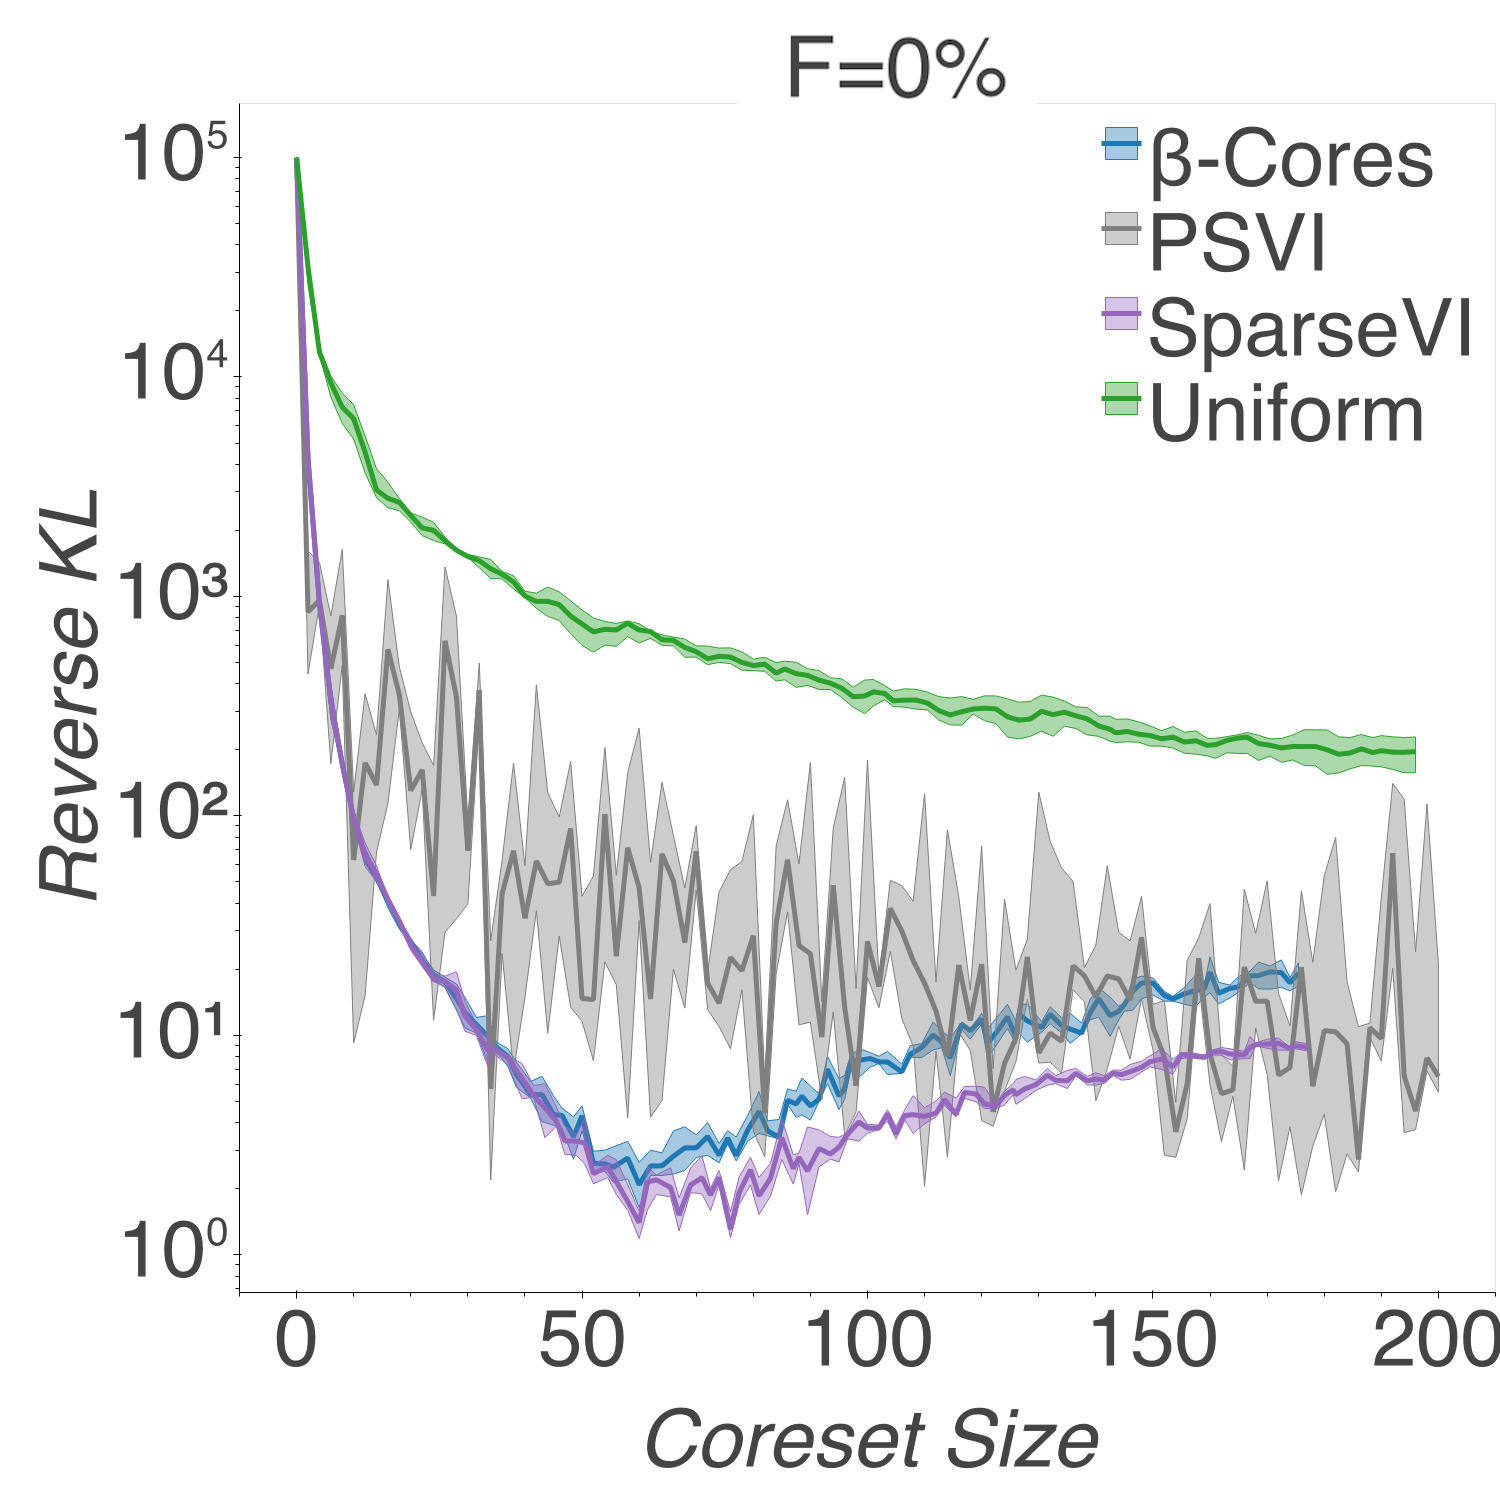
\includegraphics[width=.32\textwidth]{\MyPath/figs/f0KLDvsCstSize.png}
		\centering
		\hfill
		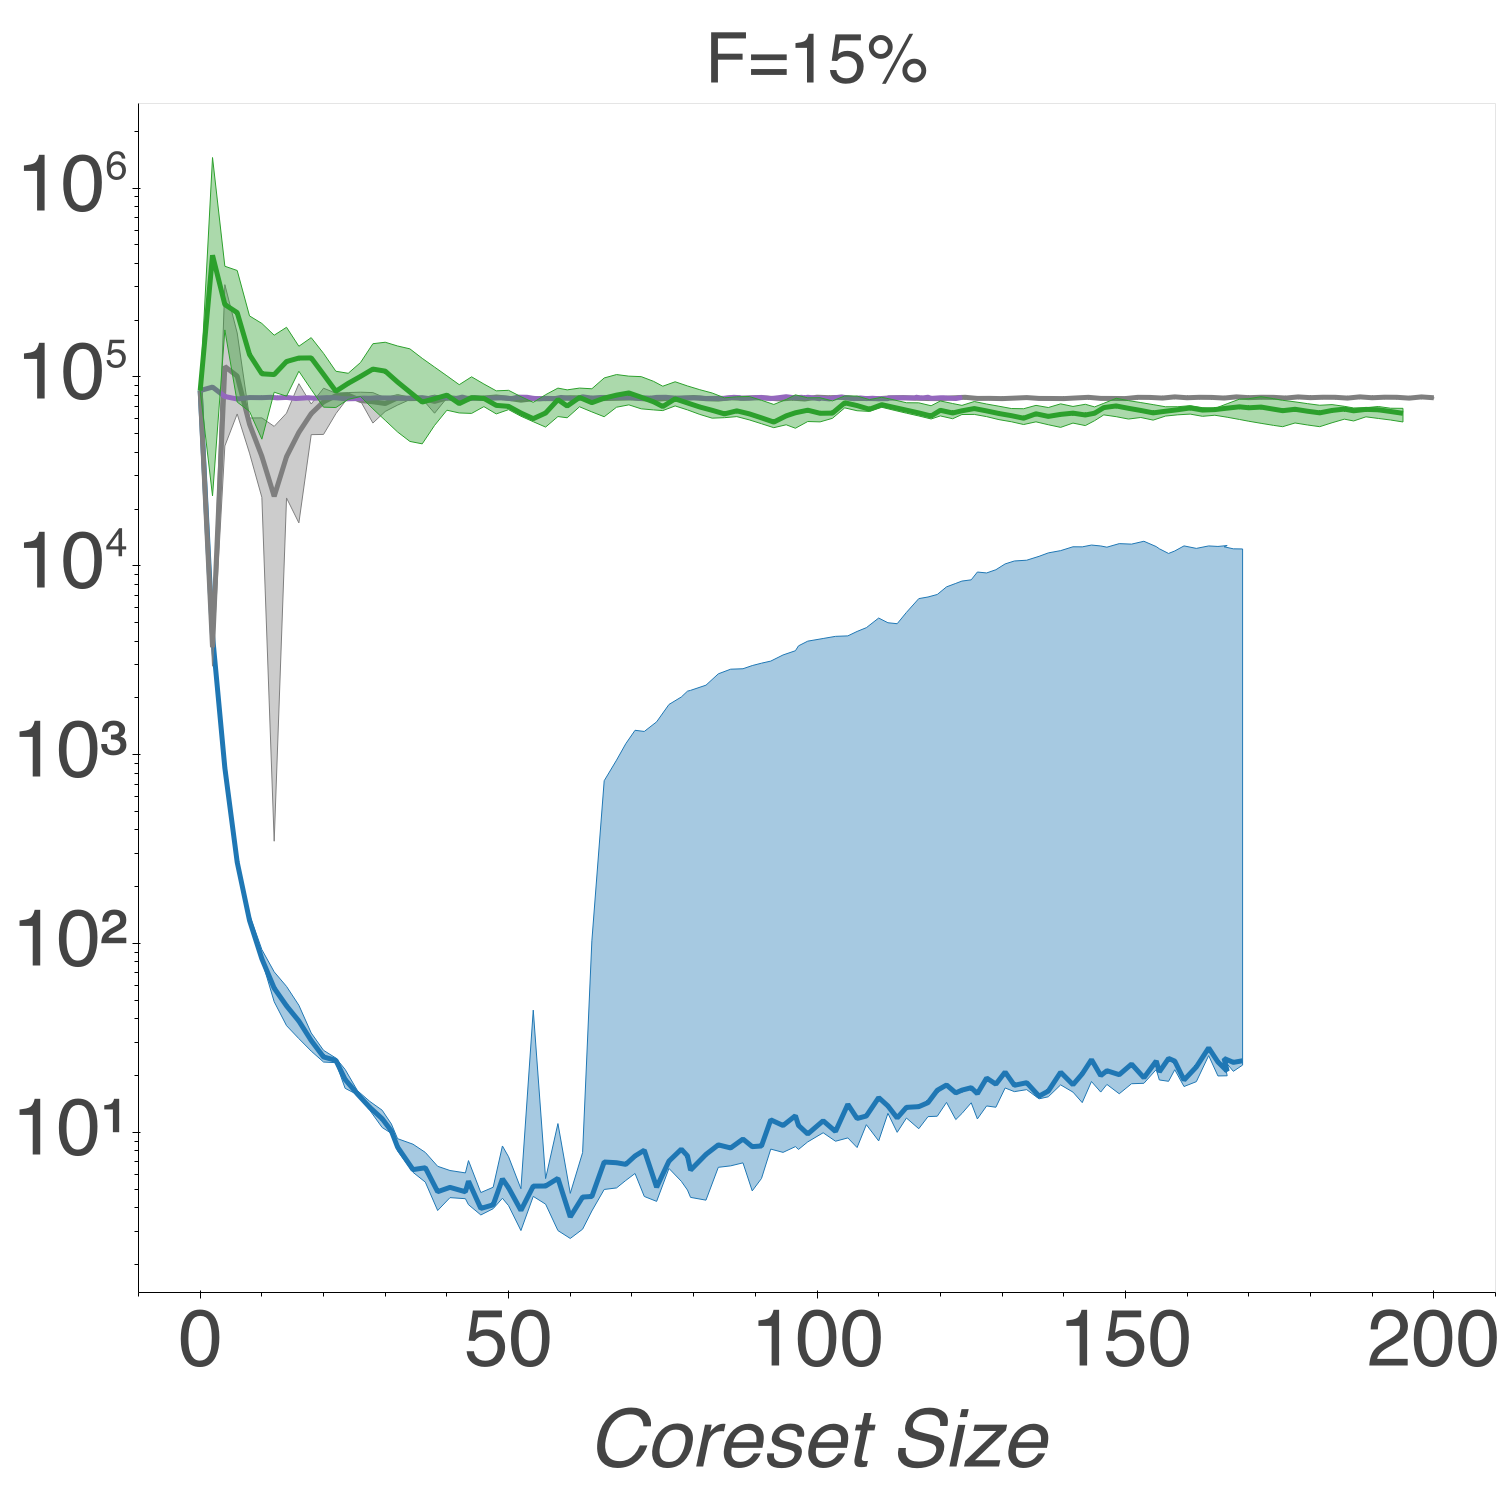
\includegraphics[width=.32\textwidth]{\MyPath/figs/f15KLDvsCstSize.png}
		\centering
		\hfill
		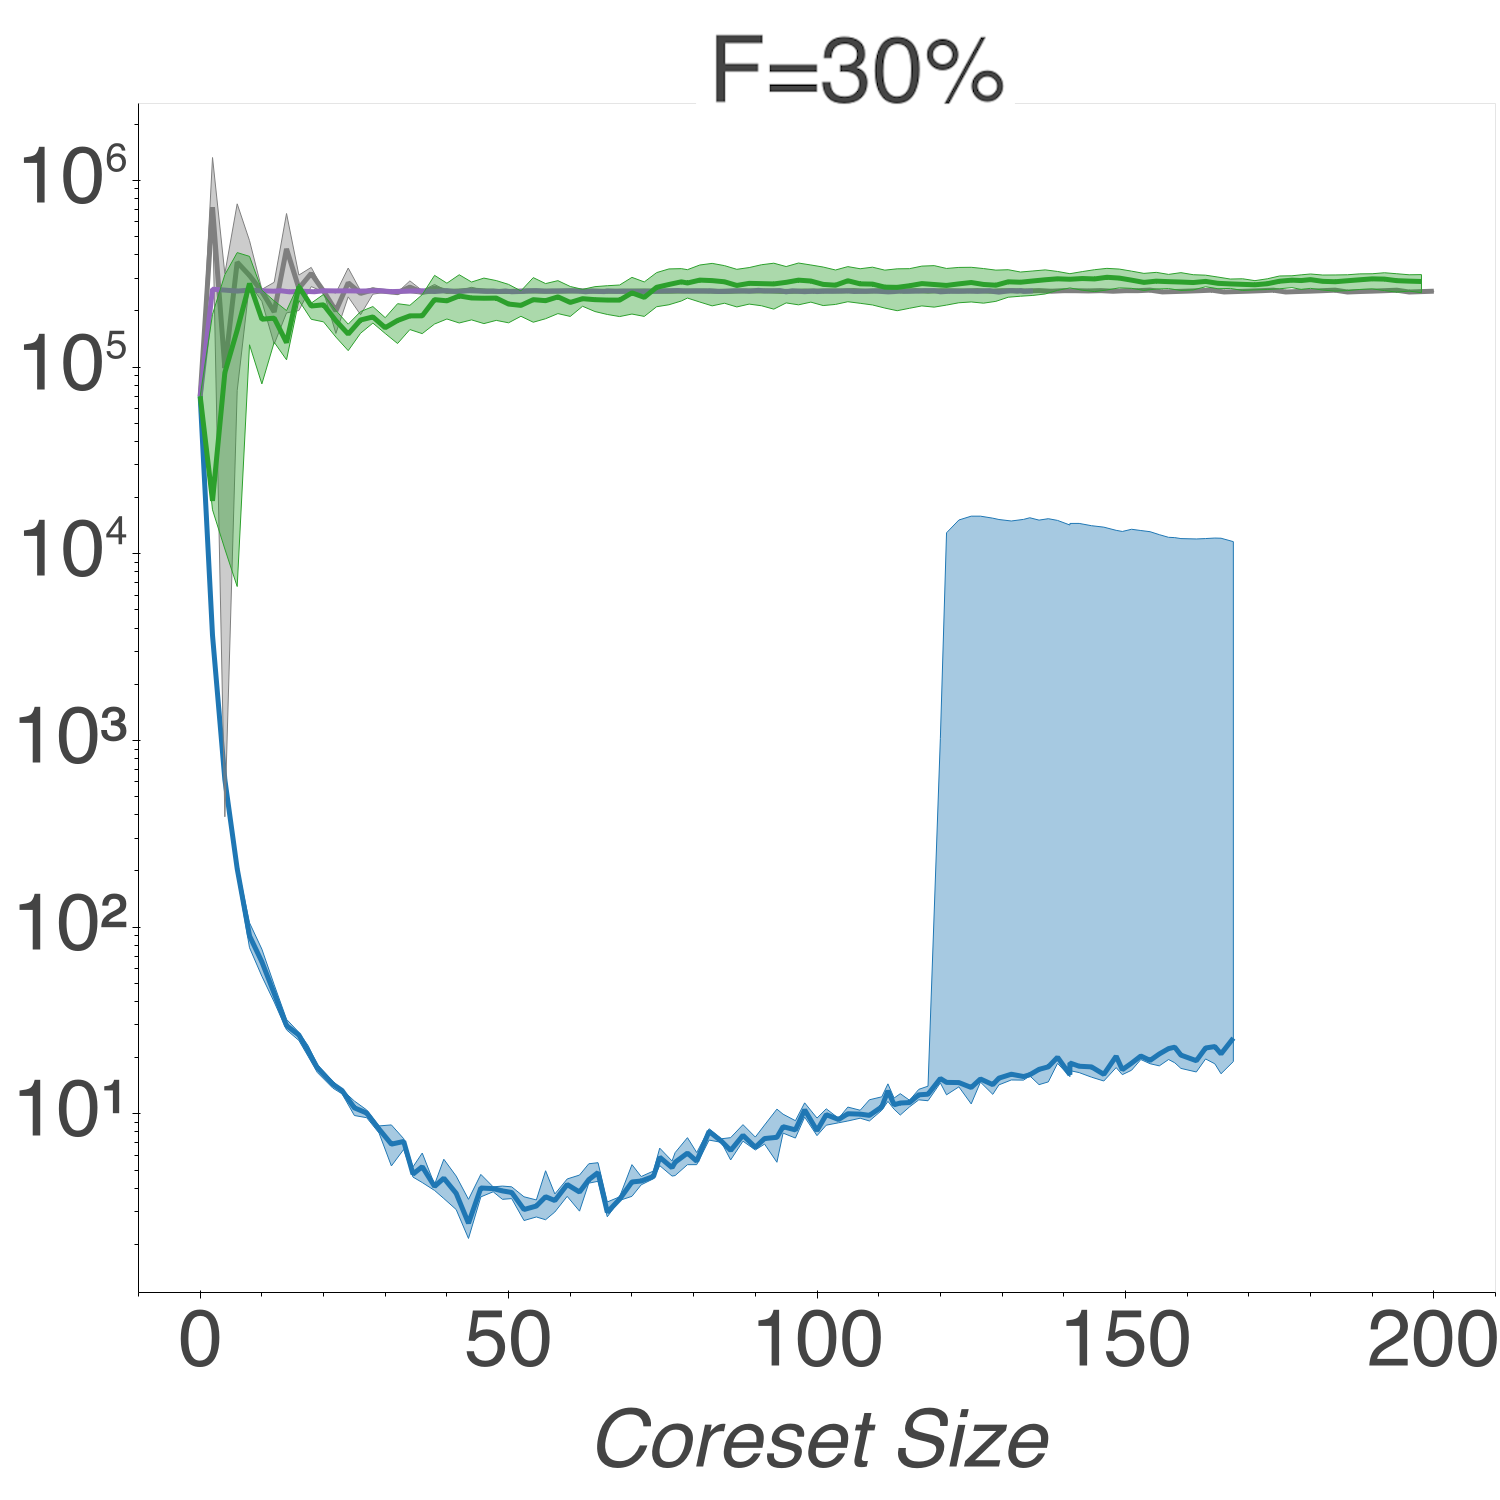
\includegraphics[width=.32\textwidth]{\MyPath/figs/f30KLDvsCstSize.png}
		\caption{\label{fig:gauss_kld}}
	\end{subfigure}	
	\centering
	\caption{(a)~Scatterplot of the observed datapoints projected on two random axes, overlaid by the corresponding coreset points and predictive posterior $3\sigma$ ellipses for increasing coreset size (from left to right). Exact posterior (illustrated in black) is computed on the dataset after removing the group of outliers. From top to bottom, the level of structured contamination increases. Classic Riemannian coresets are prone to model misspecification, adding points from the outlying component, while \bcores{} adds points only from the uncontaminated subpopulation yielding better posterior estimation. (b) Reverse KL divergence between coreset and true posterior (the latter computed on clean data), averaged over $5$ trials. Solid lines display the median KL divergence, with shaded areas showing $25\textsuperscript{th}$ and $75\textsuperscript{th}$ percentiles of KL divergence.}
\end{figure}

All computations involved in the coreset construction and posterior evaluation in this experiment can be performed in closed form. We apply the minibatch scheme of~\cref{alg:bcores}, sampling from the exact coreset posterior over gradient estimation. The used \mbox{($\beta$-)}likelihood equations are outlined in~\cref{sec:gauss-lik}. For all coreset methods, constructions are repeated for up to $M=200$ iterations, with learning rate $\gamma_t = t^{-1}$. Notice that our setting does not imply that maximum summary size contains 200 datapoints: often over the iterations an already existing summary point may be selected again, resulting in smaller coresets. Moreover, as opposed to the Gaussian experiment of the previous chapter, here we select a simpler hyperparameter selection scheme with constant initial learning rate over the entire range of coreset sizes, which in our settings allows~\sparsevi~and~\bcores~to reach their maximum posterior approximation quality at approximately 60 coreset points, and causes a slight increase in KL beyond this size.

\cref{fig:beta_gaussian_coreset_points}~presents the results obtained by the different coreset methods. We stress-test their performance under varying amounts of data corruption~(from top to bottom, 0\%, 15\%, and 30\% of the datapoints get replaced by outliers). We can verify that \bcores{} with $\beta=0.01$ is on par with existing Riemannian coresets in an uncontaminated dataset. Noticeably, \bcores{} remains robust to high levels of structured corruption~(even up to $30\%$ of the dataset), giving reliable posterior estimates; KL divergence plots in~\cref{fig:gauss_kld} reconfirm the superiority of inference via~\bcores{}. On the other hand, in the presence of outliers, previous Riemannian coresets' performance degrades quickly, offering similar posterior inference quality with random sampling. The KL divergence from the cleansed data posterior for existing summarizations and uniform sampling increases with observations' failure probability, as it asymptotically converges to the Bayesian posterior computed on the corrupted dataset. 


Moreover, in the case of contaminated datasets, baseline coresets are quite confident in their wrong predictive posteriors: they keep assigning the same weight to all observations and hence do not adjust their posterior uncertainty estimates, in spite of having to describe contradicting data. In contrast,~\bcores{} discards samples from the outlying group and can confidently explain the inliers, despite the smaller effective sample size: indeed,~\cref{fig:gauss_kld} shows that the achieved KL divergence from the exact posterior is at same order of magnitude regardless of failure probability. 

We can however notice that, for coreset sizes growing beyond 60 points---despite remaining consistently better compared to the baselines---\bcores{} starts to present some instability over trials in contaminated dataset instances. This effect is attributed to the small value of the $\beta$ hyperparameter  selected for the demonstration (so that this value can successfully model the case of clean data). As a result, eventually some outliers might be allowed to enter the summary for large coreset sizes. The instability can be resolved by increasing $\beta$ according to the observations' failure probability, and will be further discussed in~\cref{sec:sensitivity} 


\subsection{Bayesian logistic regression under mislabeling and feature noise}
\label{subsec:logreg-expt}

In this section, we study the robustness achieved by~\bcores{} on the problem of binary classification  under unreliable measurements and labeling. We test our methods on 3 benchmark datasets with varying dimensionality~($10$-$127$ dimensions, more details on the data are provided in~\cref{sec:data-details}). We observe data pairs $(x_n, y_n)_{n=1}^{N}$, where $x\in\reals^{d}$, $y_n \in \{-1,1\}$, and use the Bayesian logistic regression model to describe them,
\[
y_n | x_n, \theta \sim \distBern \left( \frac{1}{1+e^{-z_n^T \theta}}\right),
\qquad 
z_n:=\begin{bmatrix}
x_n \\
1
\end{bmatrix}.
\]
The closed form of \blik{} terms required in our construction is computed in~\cref{sec:logreg-lik}. 

Data corruption is simulated by generating outliers in the input and output space similarly to~\citep{futami18}: For corruption rate $F$, we sample two random subsets of size $F\cdot N$ from the training data.  For the datapoints in the first subset, we replace the value of half of the features with Gaussian noise sampled \iid from $\distNorm(0,5)$; for the datapoints in the other subset, we flip the binary label. Over construction we use Laplace approximation~\citep{mackay03} to efficiently draw samples from the (non-conjugate) coreset posterior, while over evaluation coreset posterior samples are obtained via NUTS~\citep{hoffman14}. We evaluate the accuracy over the test set, predicting labels according to the maximum log-likelihood rule under the posterior $\theta$ sampling distribution. The learning rate schedule was set to $\gamma_t=c_0 t^{-1}$, with $c_0$ set to 1 for \sparsevi{} and \bcores{}, and 0.1 for \psvi. 
The values for hyperparameter $\beta$ and learning rates $\gamma_t$ were chosen via cross-validation. 

\begin{figure}[!tp]
	\begin{subfigure}[]{0.995\textwidth} 
		\centering
		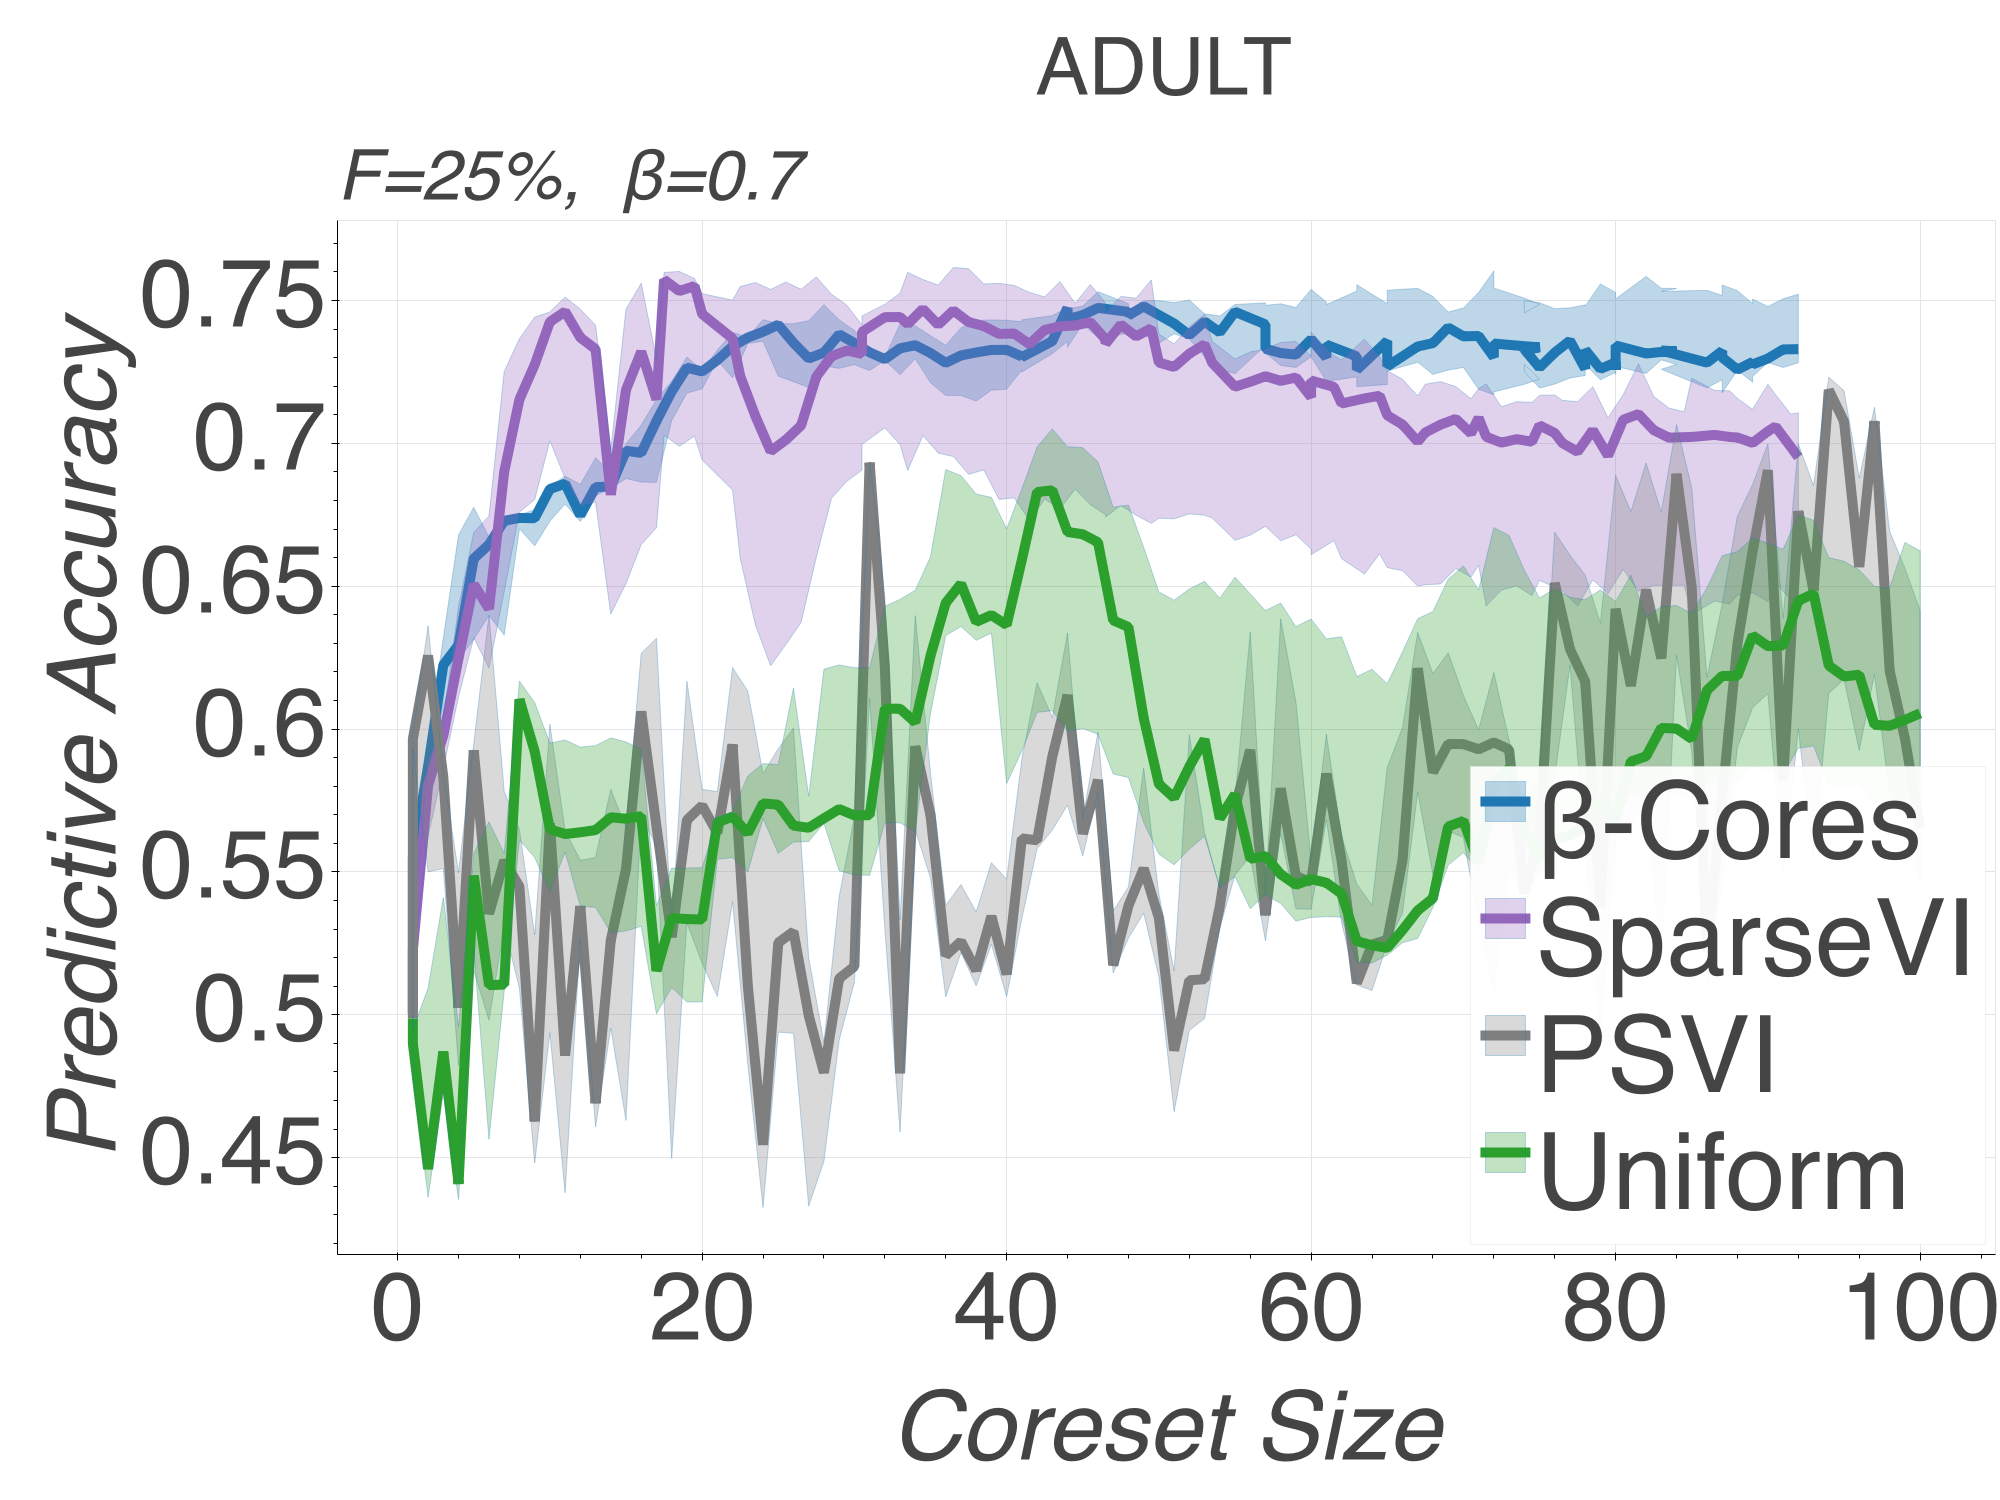
\includegraphics[width=.325\textwidth]{\MyPath/figs/adult07_10_25_False_False_ACCvssz.png}
		\centering
		\hfill
		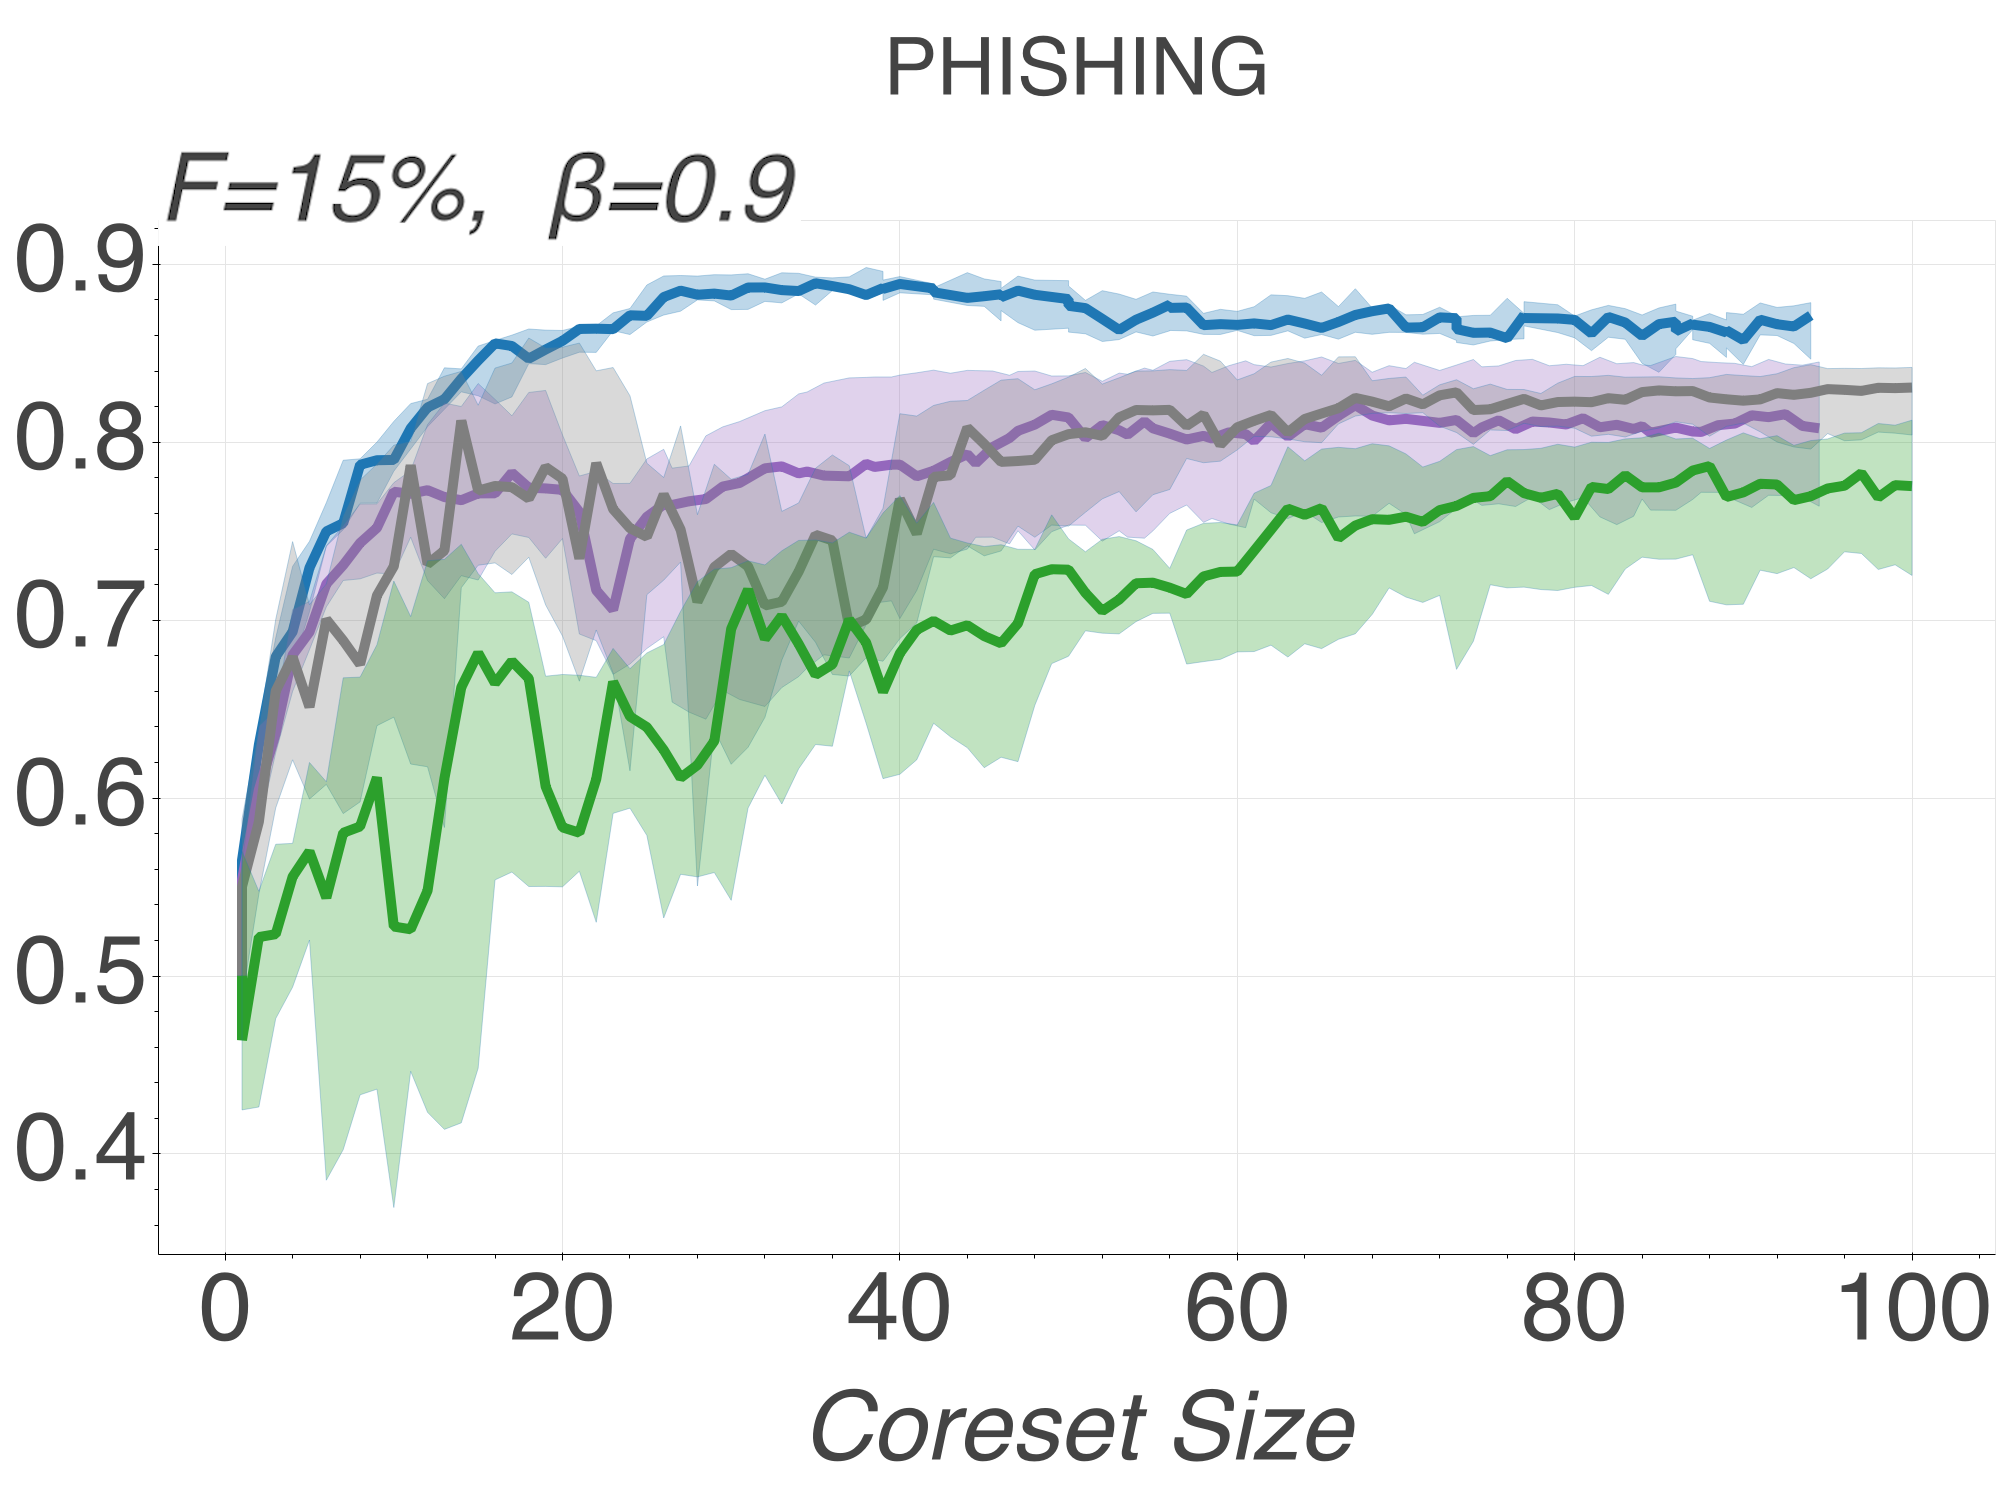
\includegraphics[width=.325\textwidth]{\MyPath/figs/phish09_10_15_False_False_ACCvssz.png}
		\centering
		\hfill
		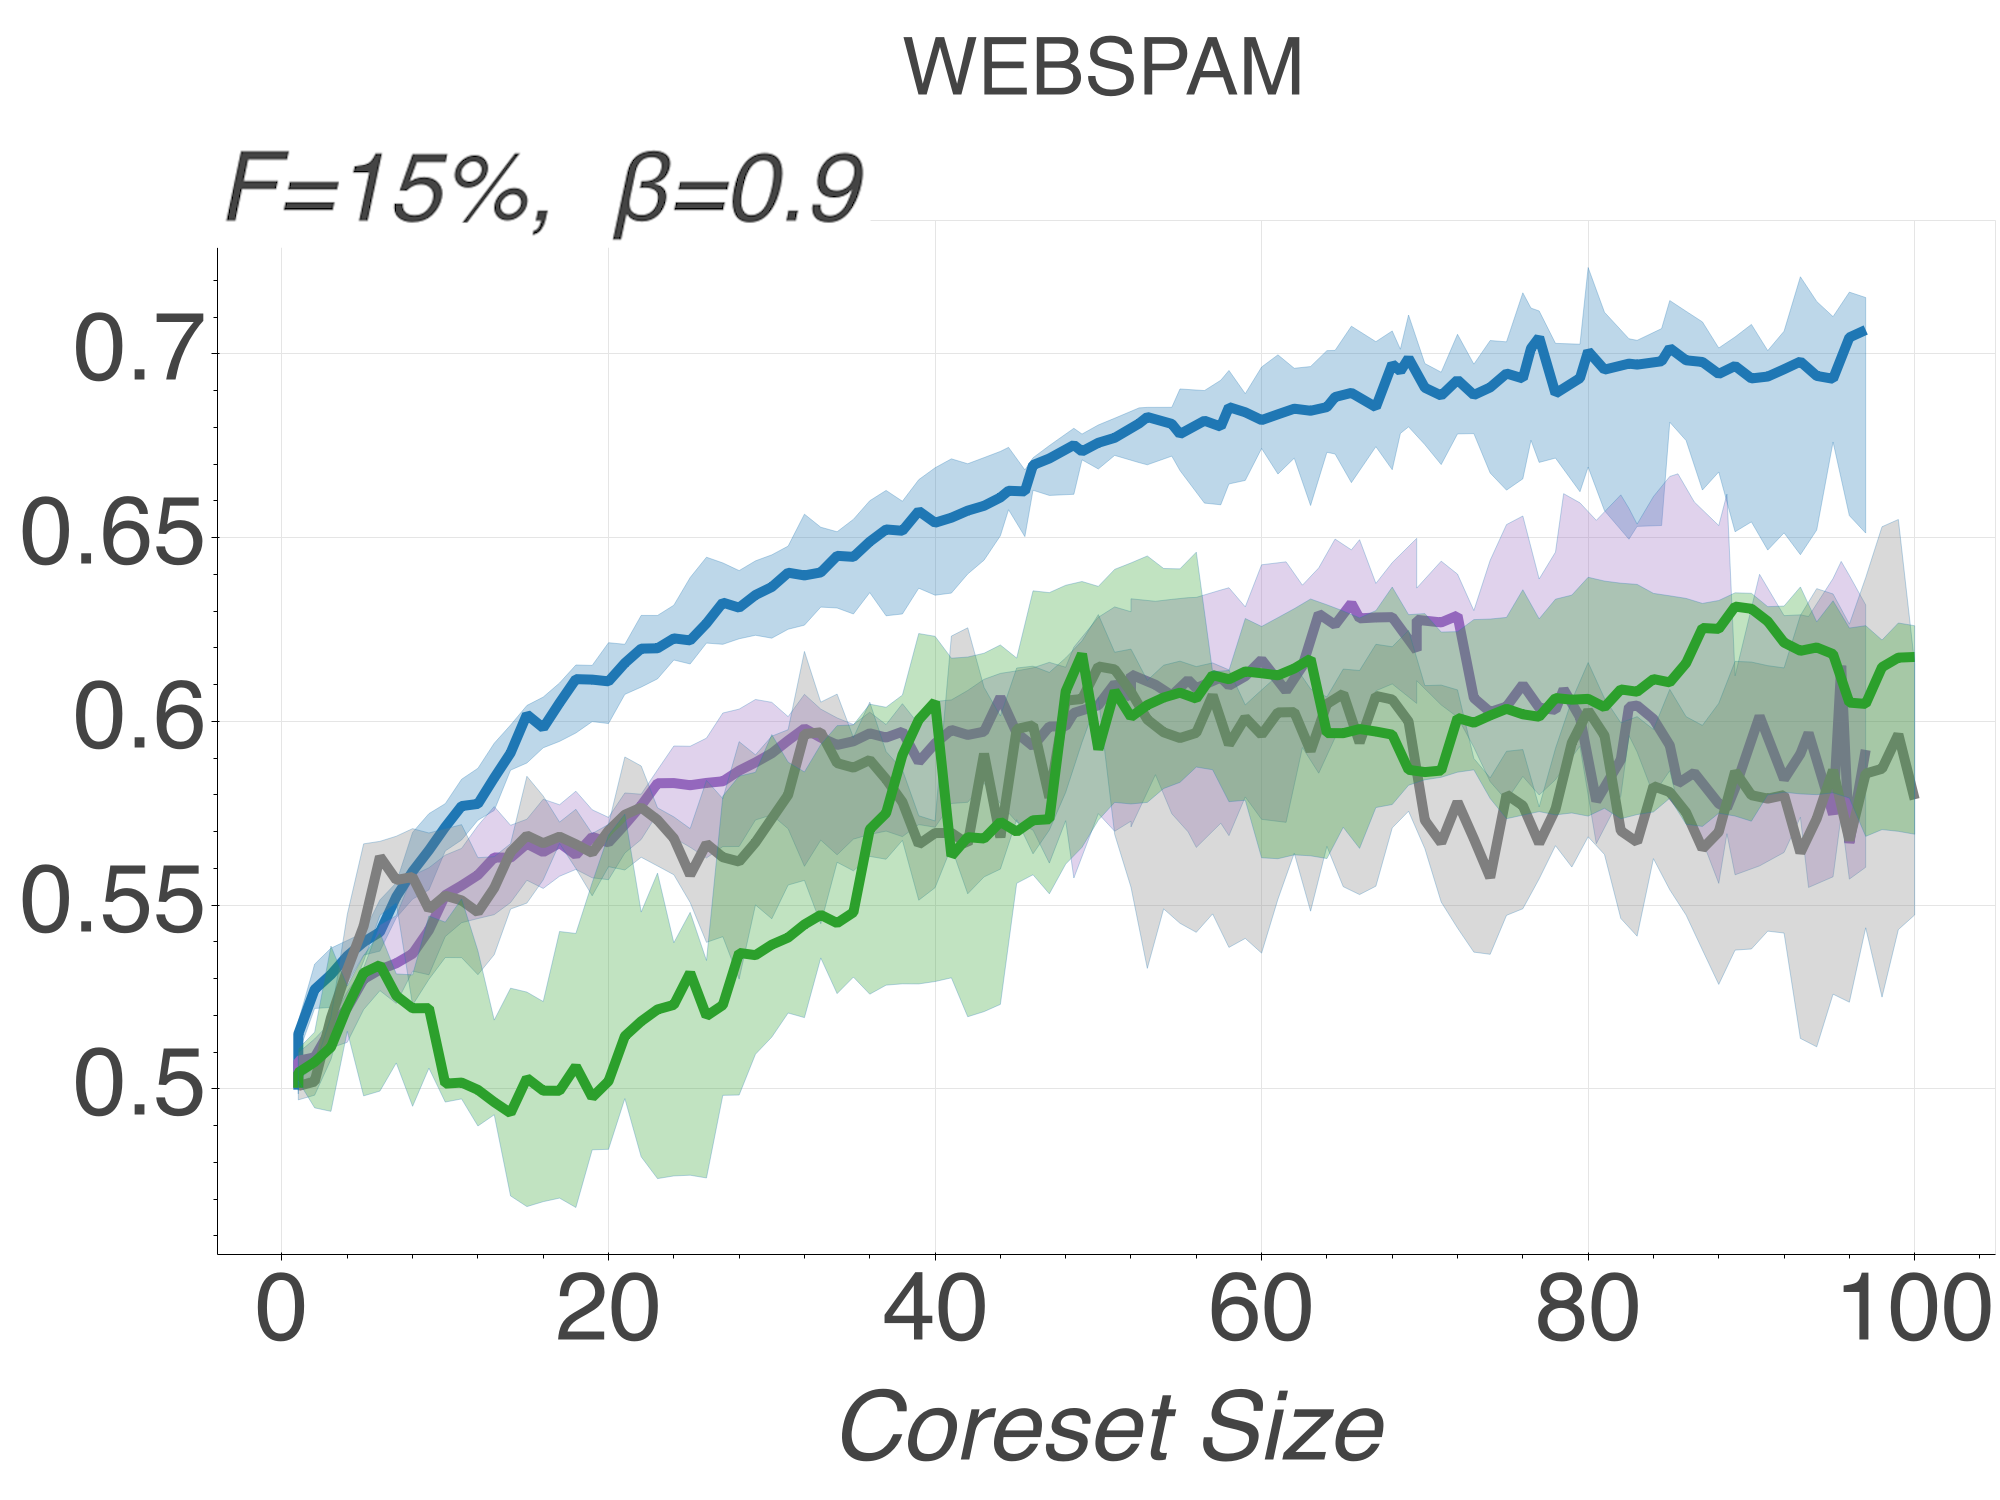
\includegraphics[width=.325\textwidth]{\MyPath/figs/webspam09_10_15_True_False_ACCvssz.png}
		\centering
		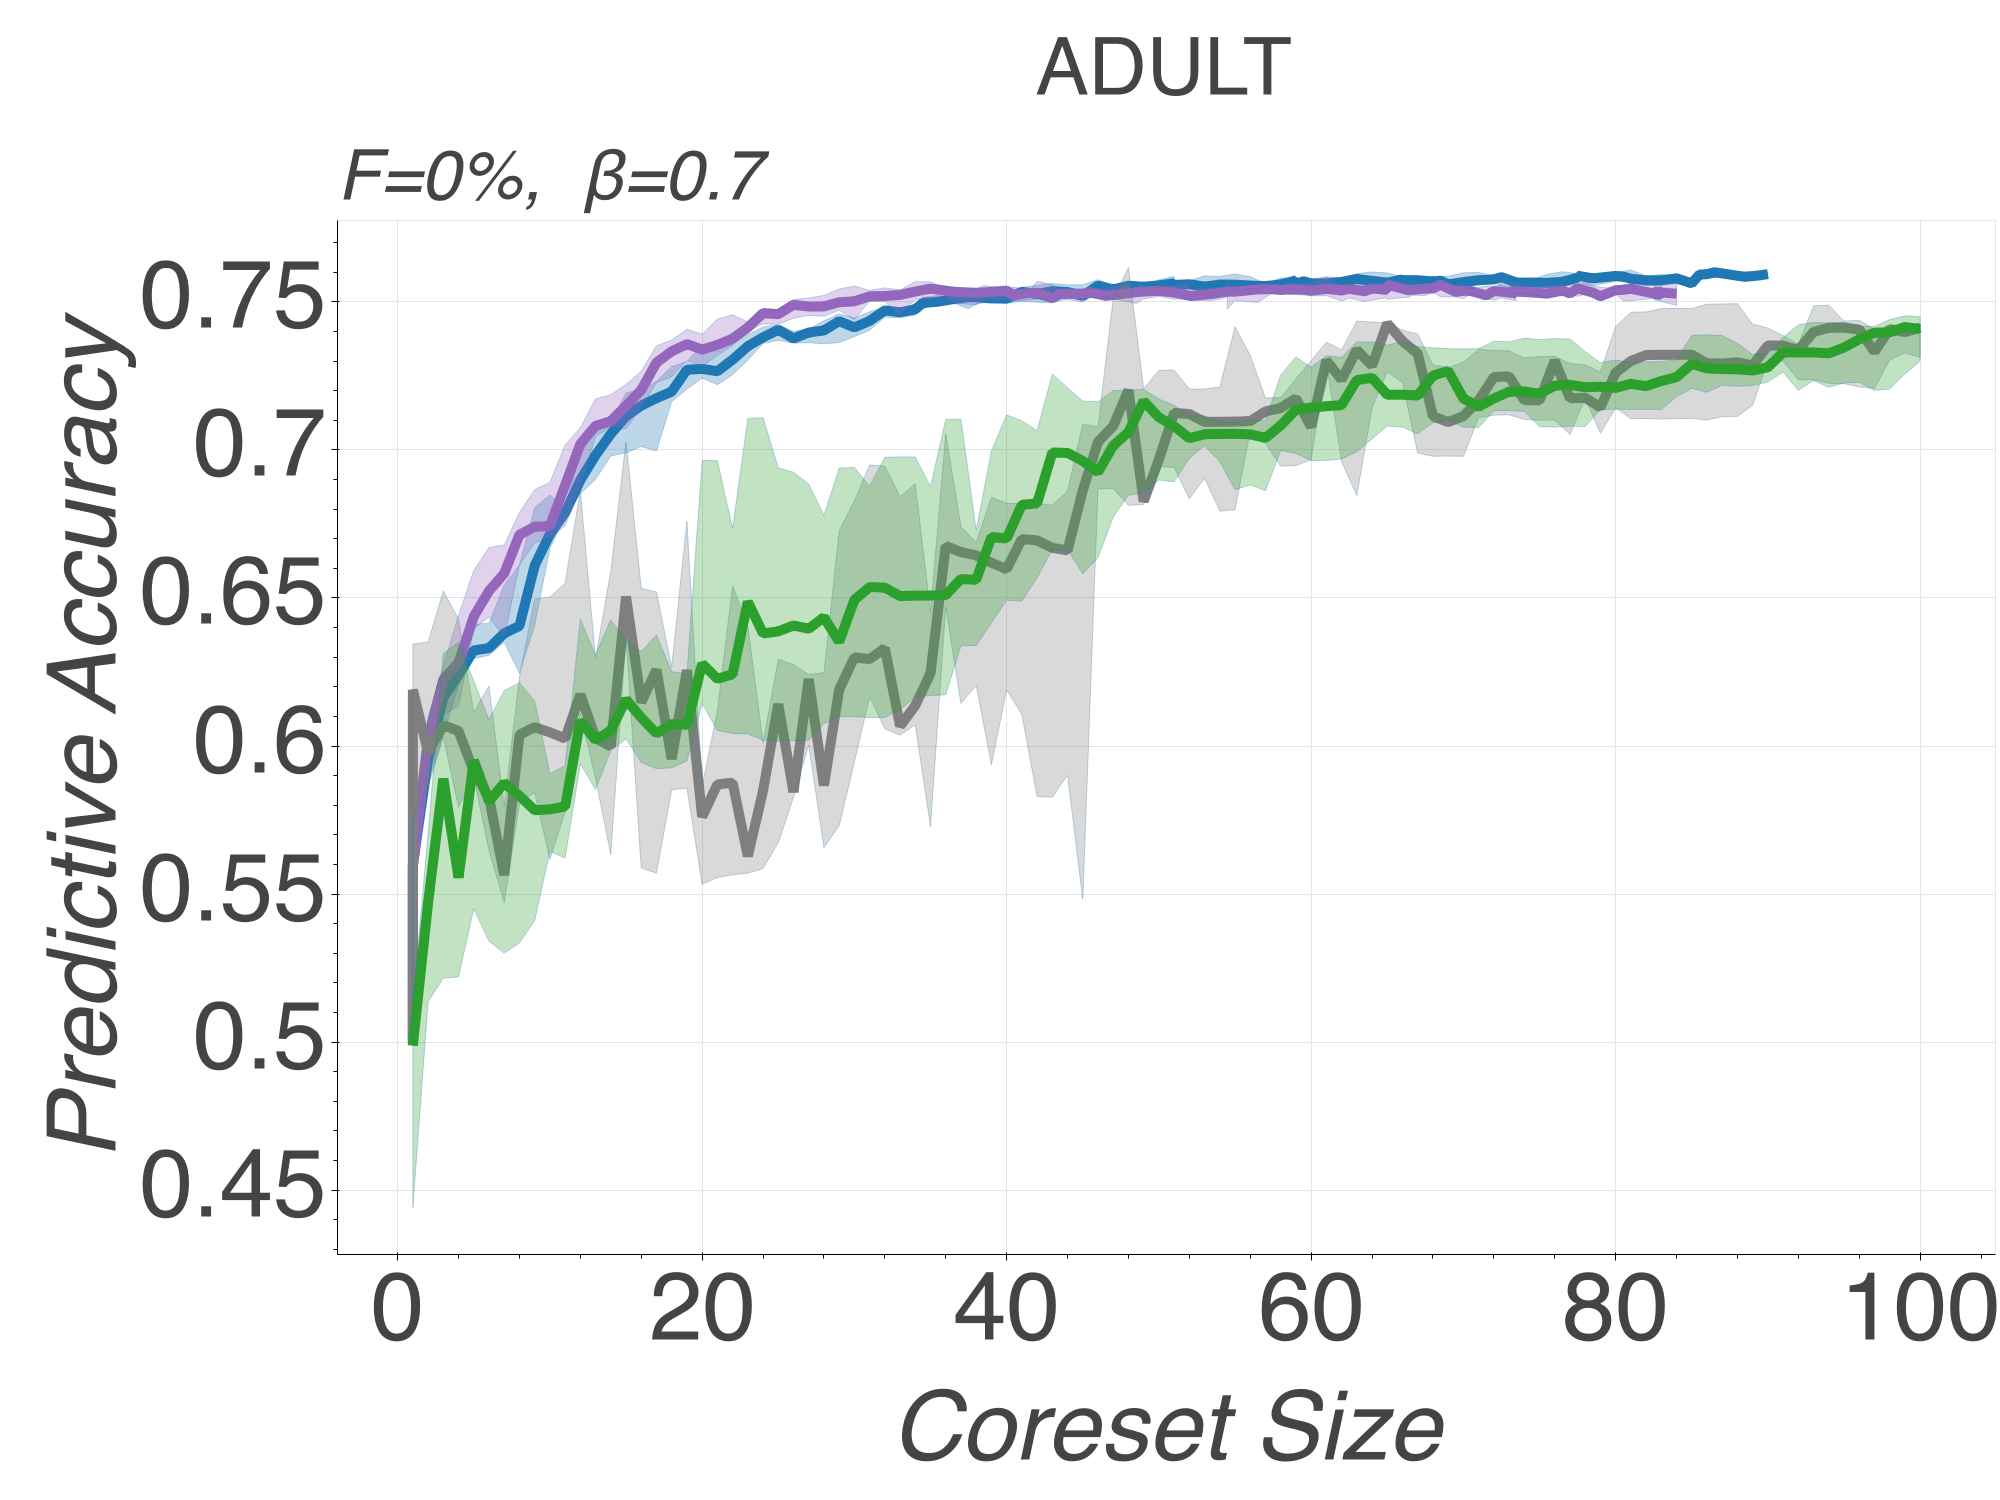
\includegraphics[width=.325\textwidth]{\MyPath/figs/adult07_10_0_False_False_ACCvssz.png}
		\centering
		\hfill
		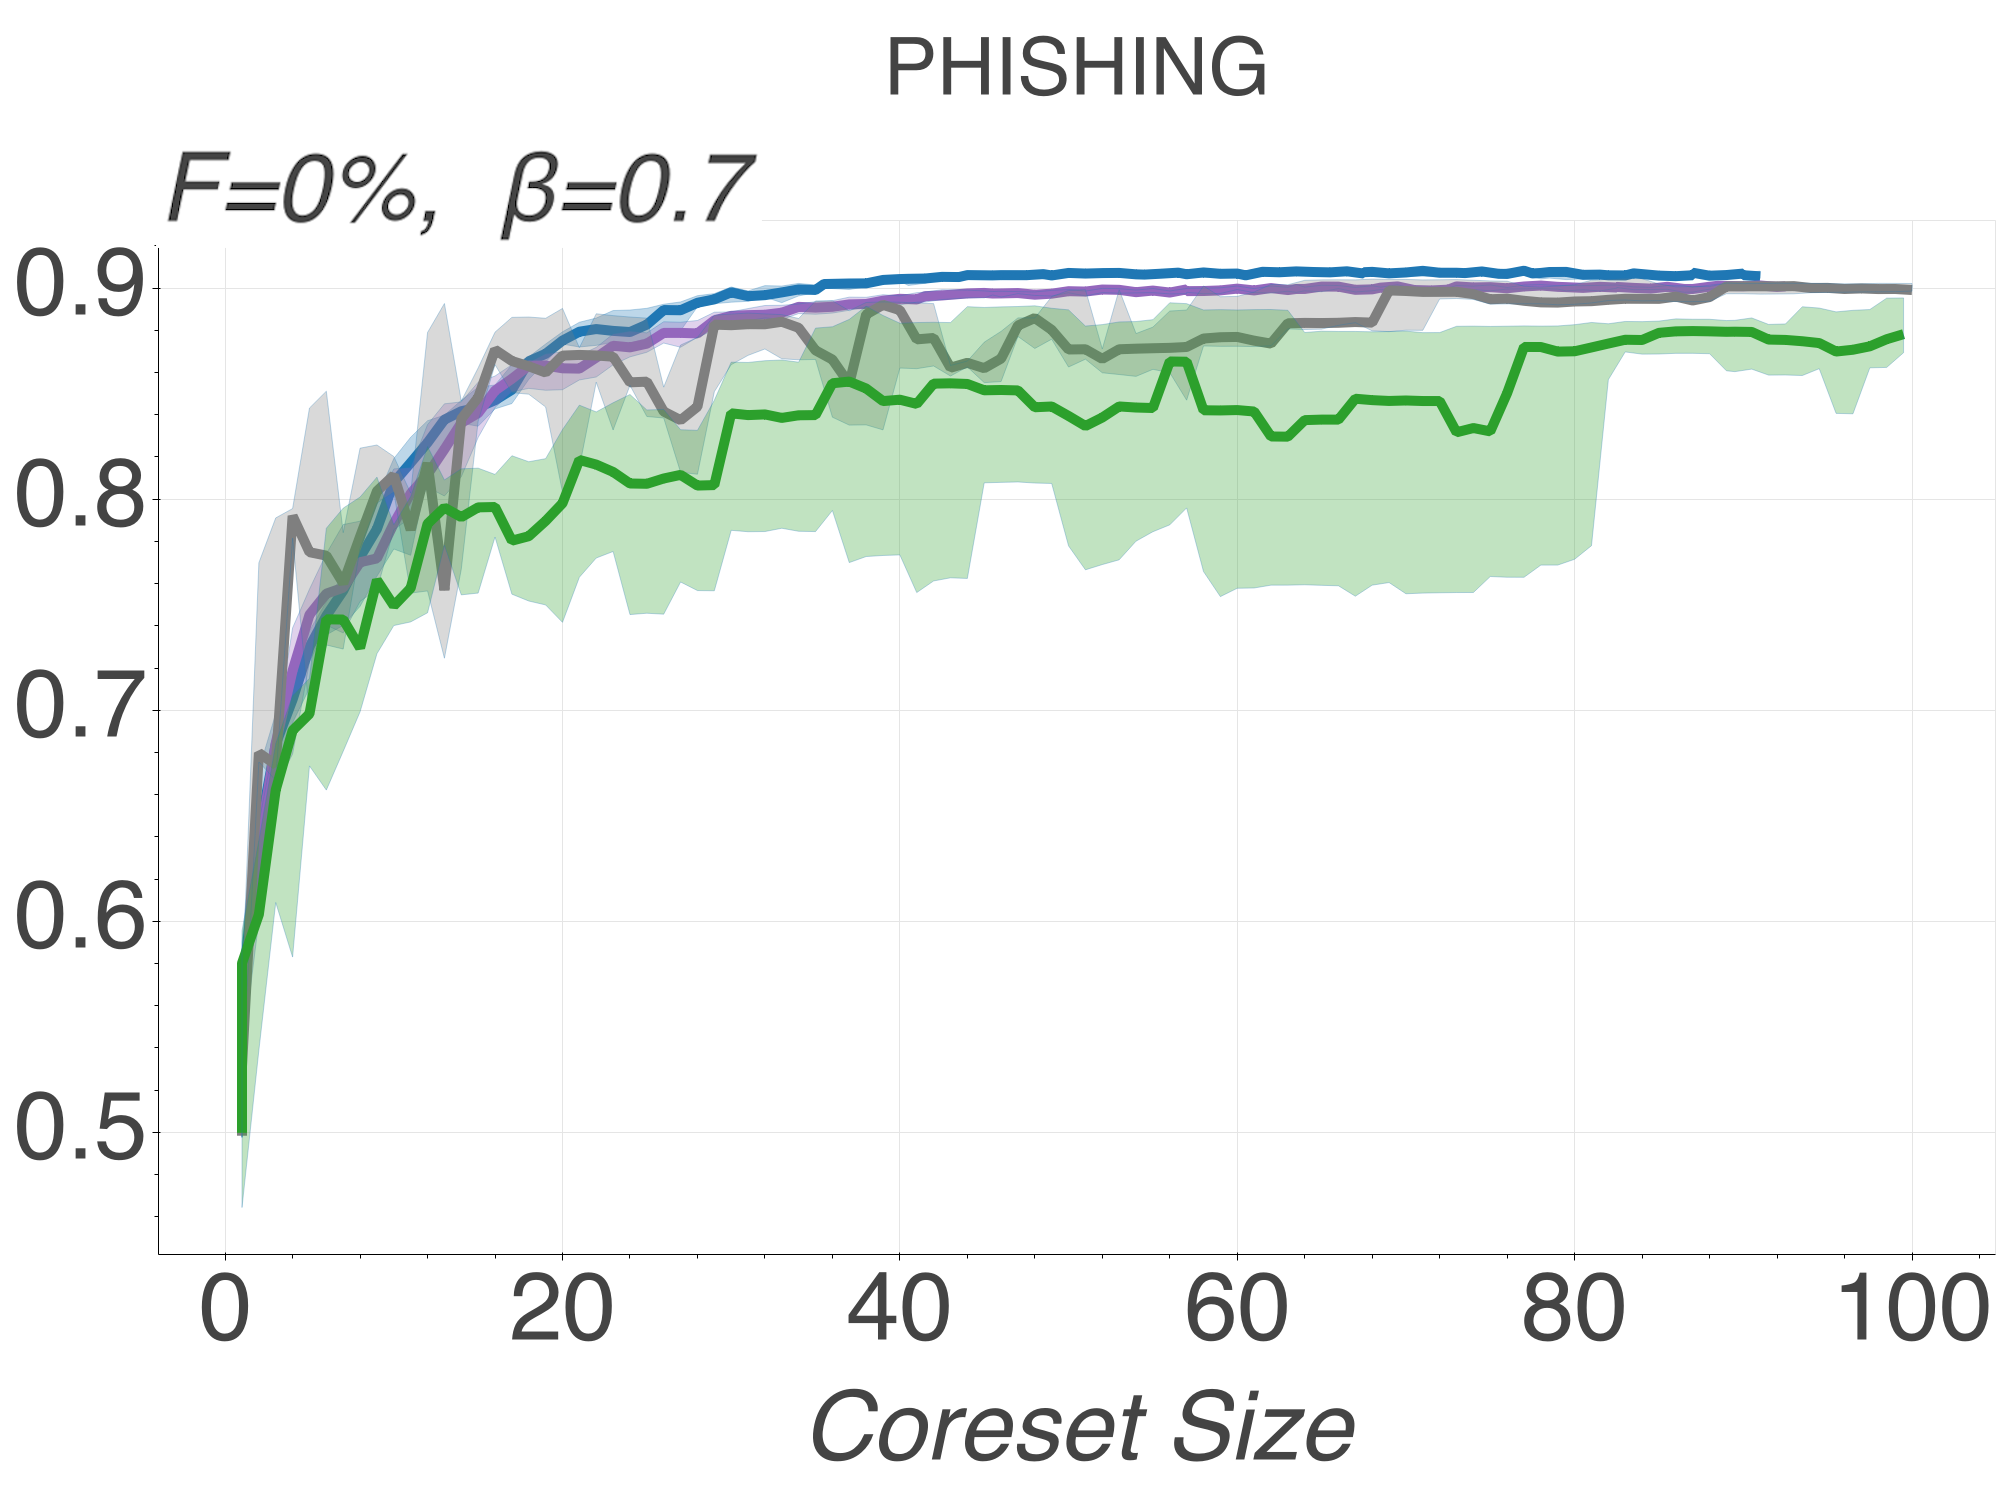
\includegraphics[width=.325\textwidth]{\MyPath/figs/phish07_10_0_False_False_ACCvssz.png}
		\centering
		\hfill
		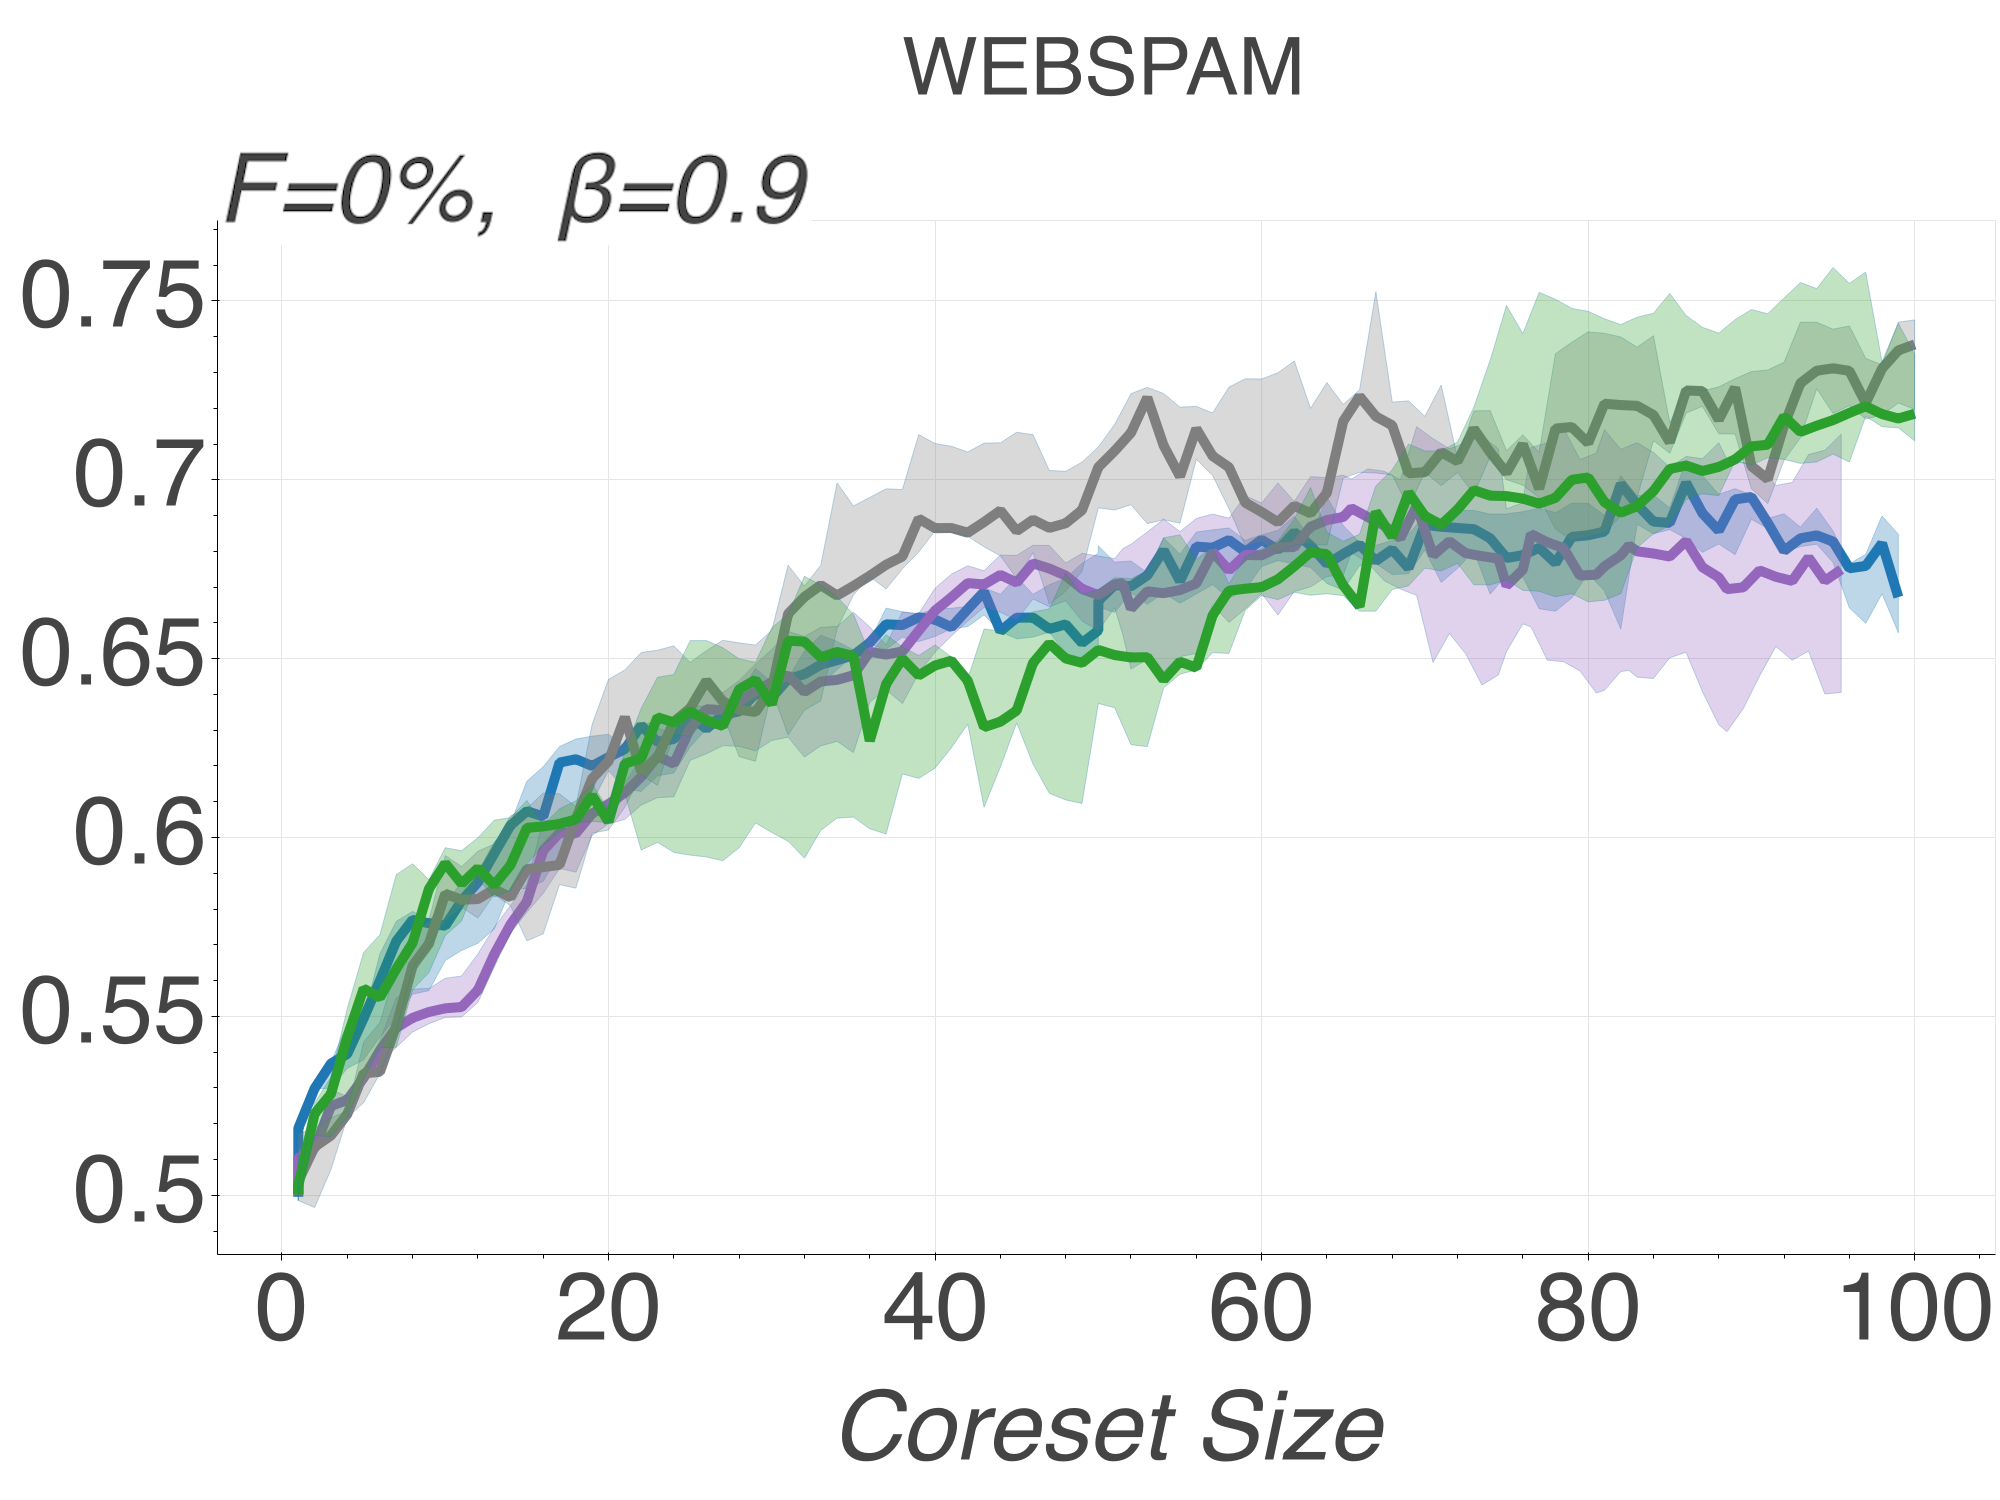
\includegraphics[width=.325\textwidth]{\MyPath/figs/webspam09_10_0_True_False_ACCvssz.png}
	\end{subfigure}	
	\centering
	\caption{Predictive accuracy vs coreset size for logistic regression experiments over $10$ trials on $3$ large-scale datasets. Solid lines display the median accuracy, with shaded areas showing $25\textsuperscript{th}$ and $75\textsuperscript{th}$ percentiles. Dataset corruption rate $F$, and $\beta$ value used in \bcores{} for each experiment are shown on the figures. The bottom row plots illustrate the achieved predictive performance under no contamination.}
	\label{fig:logreg_plot}
\end{figure}

\cref{fig:logreg_plot} illustrates that \bcores{} shows competitive performance with the classical Riemannian coresets in the absence of data contamination~(bottom row), while it consistently achieves the best predictive accuracy in corrupted datasets~(top row).  On the other hand, ordinary summarization techniques, although overall outperforming random sampling for small coreset sizes, soon attain degraded predictive performance on poisoned data: by construction, via increasing coreset size, Riemannian coresets are expected to converge to the Bayesian posterior computed on the corrupted dataset. All baselines present noticeable degradation in their predictive accuracy when corruption is introduced (typically more than $5\%$), which is not the case for our method: \bcores{} is designed to support corrupted input and, for a well-tuned hyperparameter $\beta$, maintains similar performance in the presence of outliers, while practically it can even achieve improvement (as occurring for the \textsc{WebSpam} data).
%\footnote{For~\textsc{WebSpam} we notice that coresets performance in uncontaminated data for the displayed summary sizes is comparable to uniform sampling: this is a side effect of the high-dimensionality of this dataset examined in more depth at~\citep{psvi}, which out of scope for the purposes of this work.},


\subsection{Neural linear regression on noisy data batches}
\label{subsec:neur-linr-expt}

Here we use the coresets extension for batch summarization to efficiently train a neural linear model on selected data minibatches. Neural linear models perform Bayesian linear regression on the representation of the last layer of a deterministic neural network feature extractor~\citep{snoek15,riquelme18,pinsler19}.
The corresponding statistical model is as follows
\[
%&z(\cdot) \dist \distNorm(\mu_0, \sigma_0^2 I), \\
%\quad 
&\left(y_n\right)_{n=1}^{N} = \theta^T z(x_n) + \eps_n,
\quad
\left(\eps_n\right)_{n=1}^{N} \dist \distNorm(0, \sigma^2).
\label{eq:neurlinr-stat-model}
\]
The neural network is trained to learn an adaptive basis $z(\cdot)$ from $N$ datapoint pairs $(x_n,y_n) \in \reals^{d} \times \reals$, which we then use to regress $ \left(y_n\right)_{n=1}^{N} $ on $ \left(z(x_n)\right)_{n=1}^{N} $, and yield uncertainty aware estimates of $\theta$. More details on the model-specific formulae entering coresets construction are provided in~\cref{sec:neurlinr-lik}. Input and output related outliers are simulated as in~\cref{subsec:logreg-expt}, while here, for the output related outliers, $y_n$  gets replaced by Gaussian noise. Corruption occurs over a percentage $F\%$ of the total number of minibatches of the dataset, while the remaining minibatches are left uncontaminated. Each poisoned minibatch gets $70\%$ of its points \mbox{substituted by outliers}.

\begin{figure*}[!t]
	\begin{subfigure}[b]{0.99\textwidth} 
		\centering
		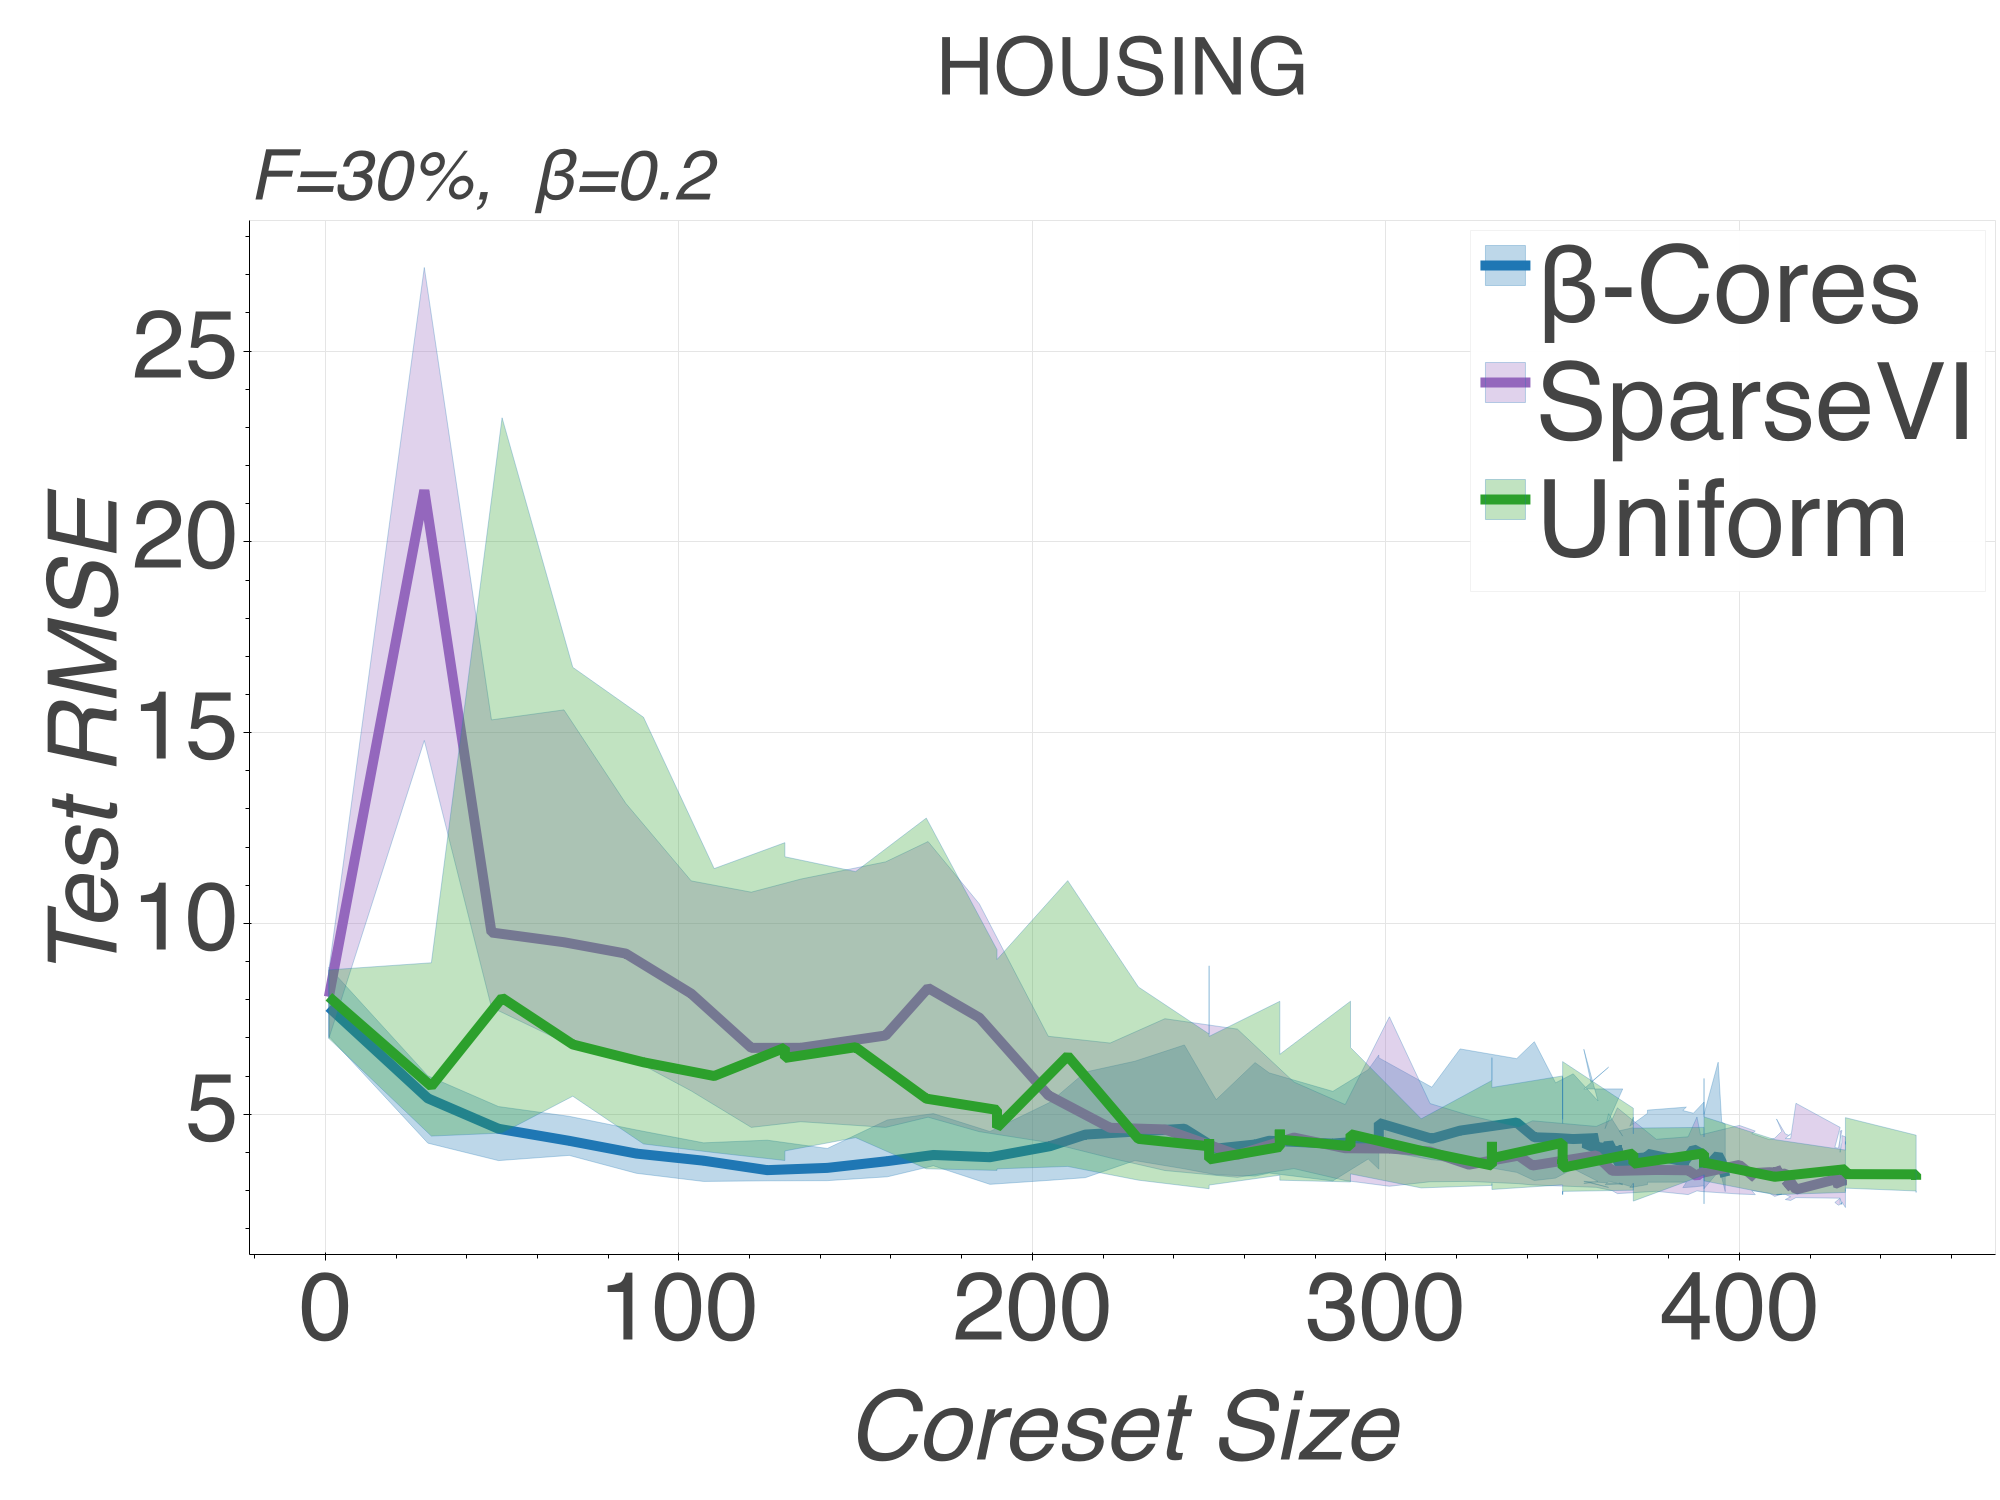
\includegraphics[width=.47\textwidth]{\MyPath/figs/boston02_01_30_RMSEvssz.png}
		\hfill
		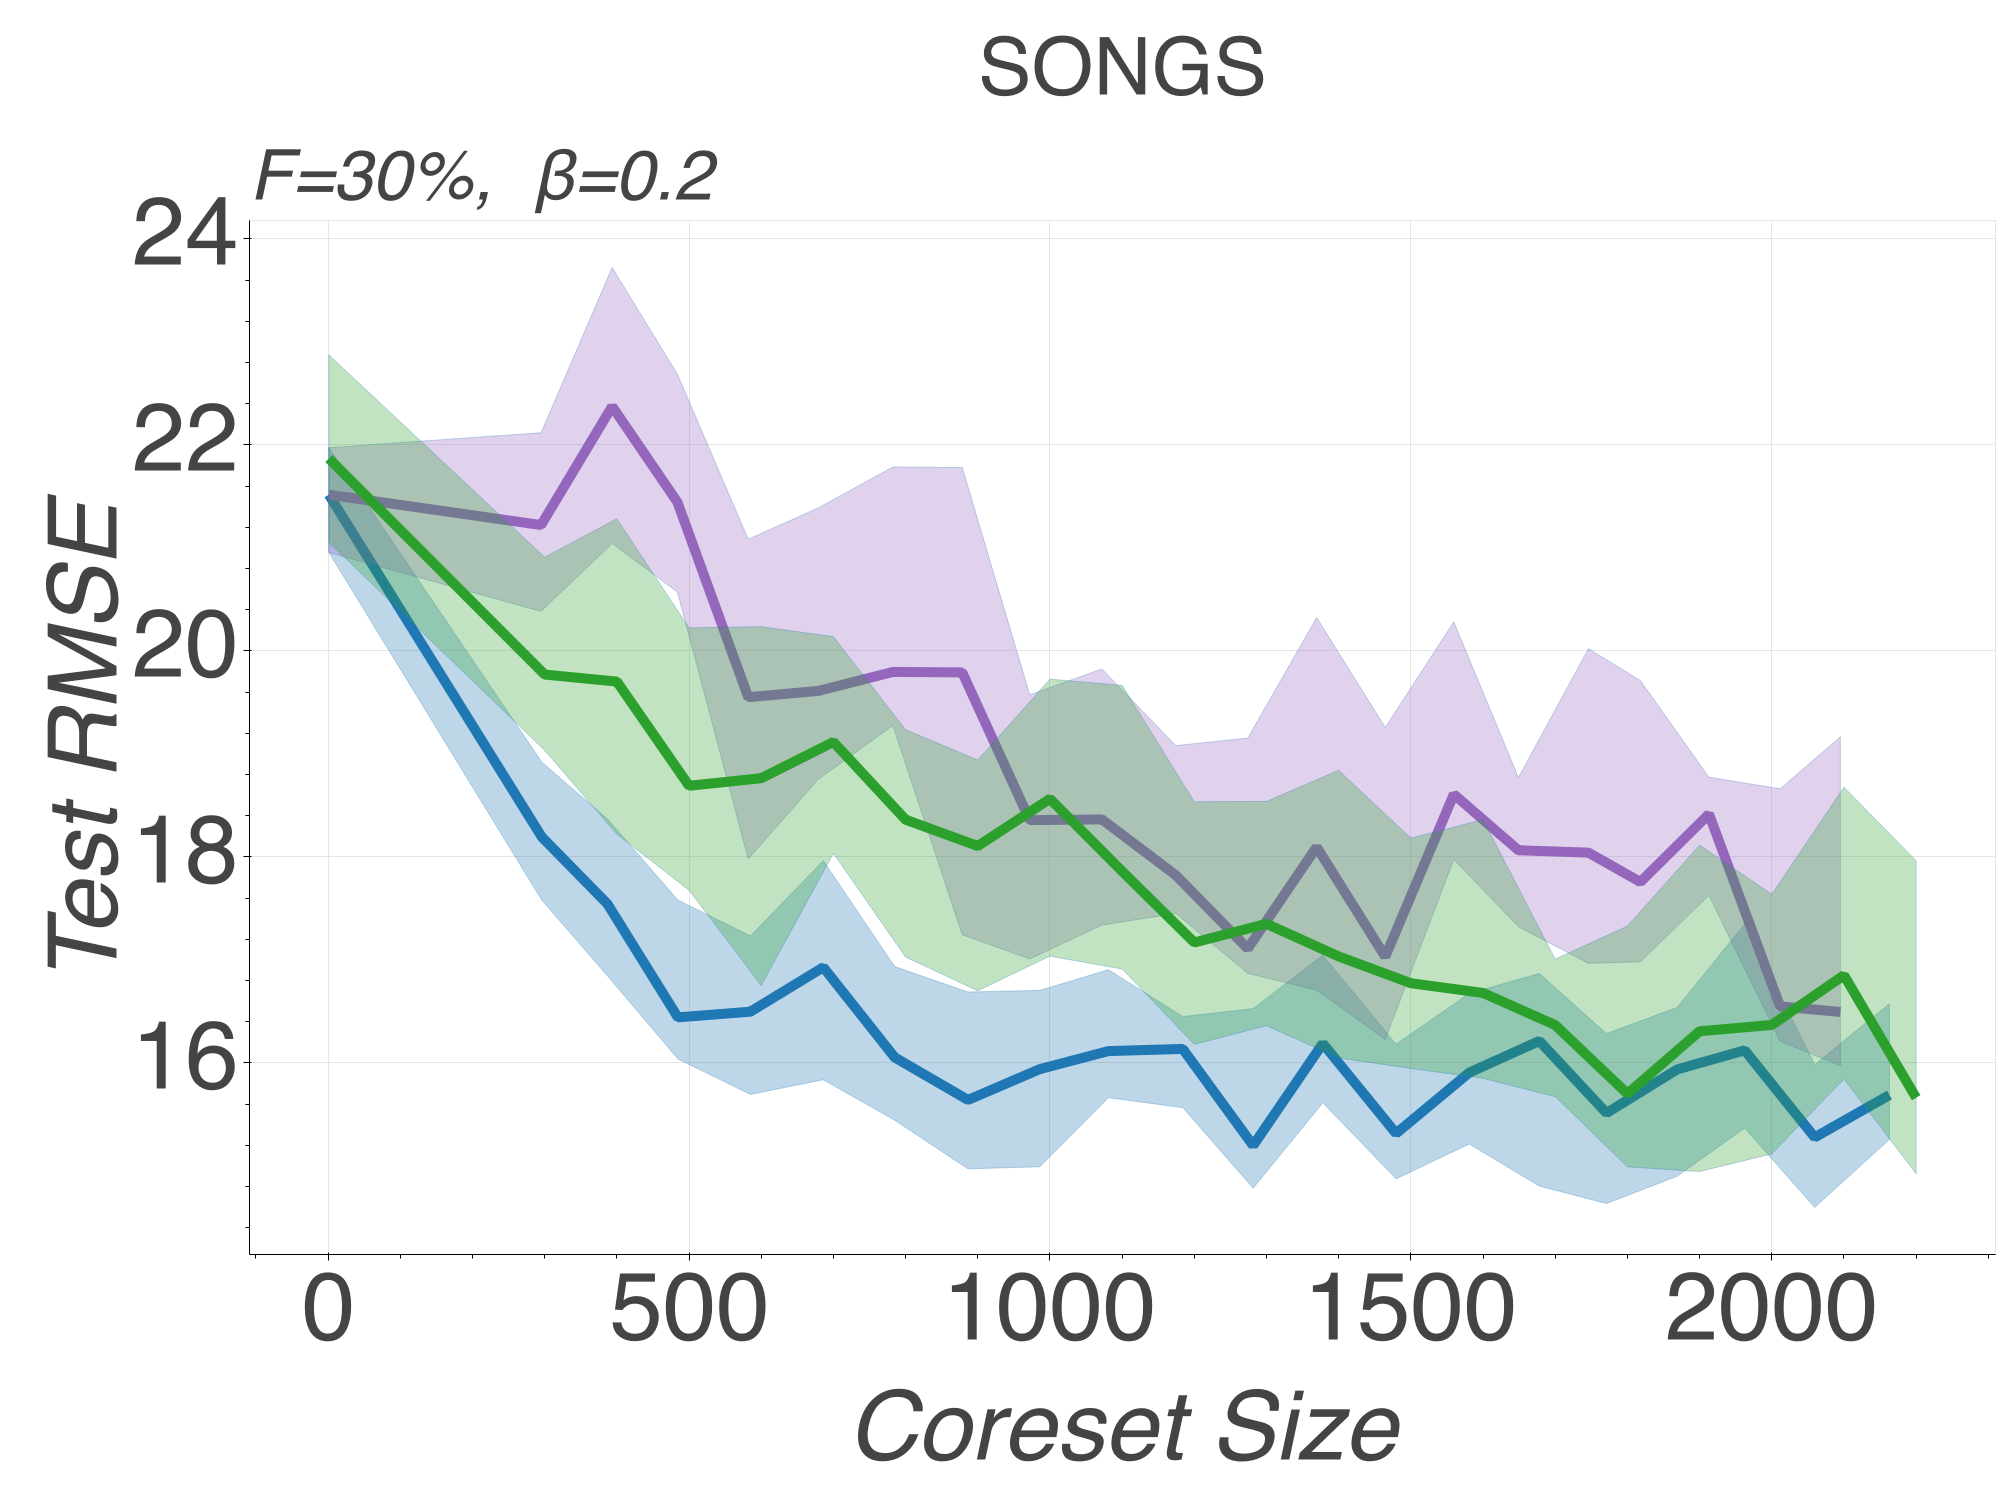
\includegraphics[width=.47\textwidth]{\MyPath/figs/year02_01_30_RMSEvssz.png}
		\centering
		\hfill
		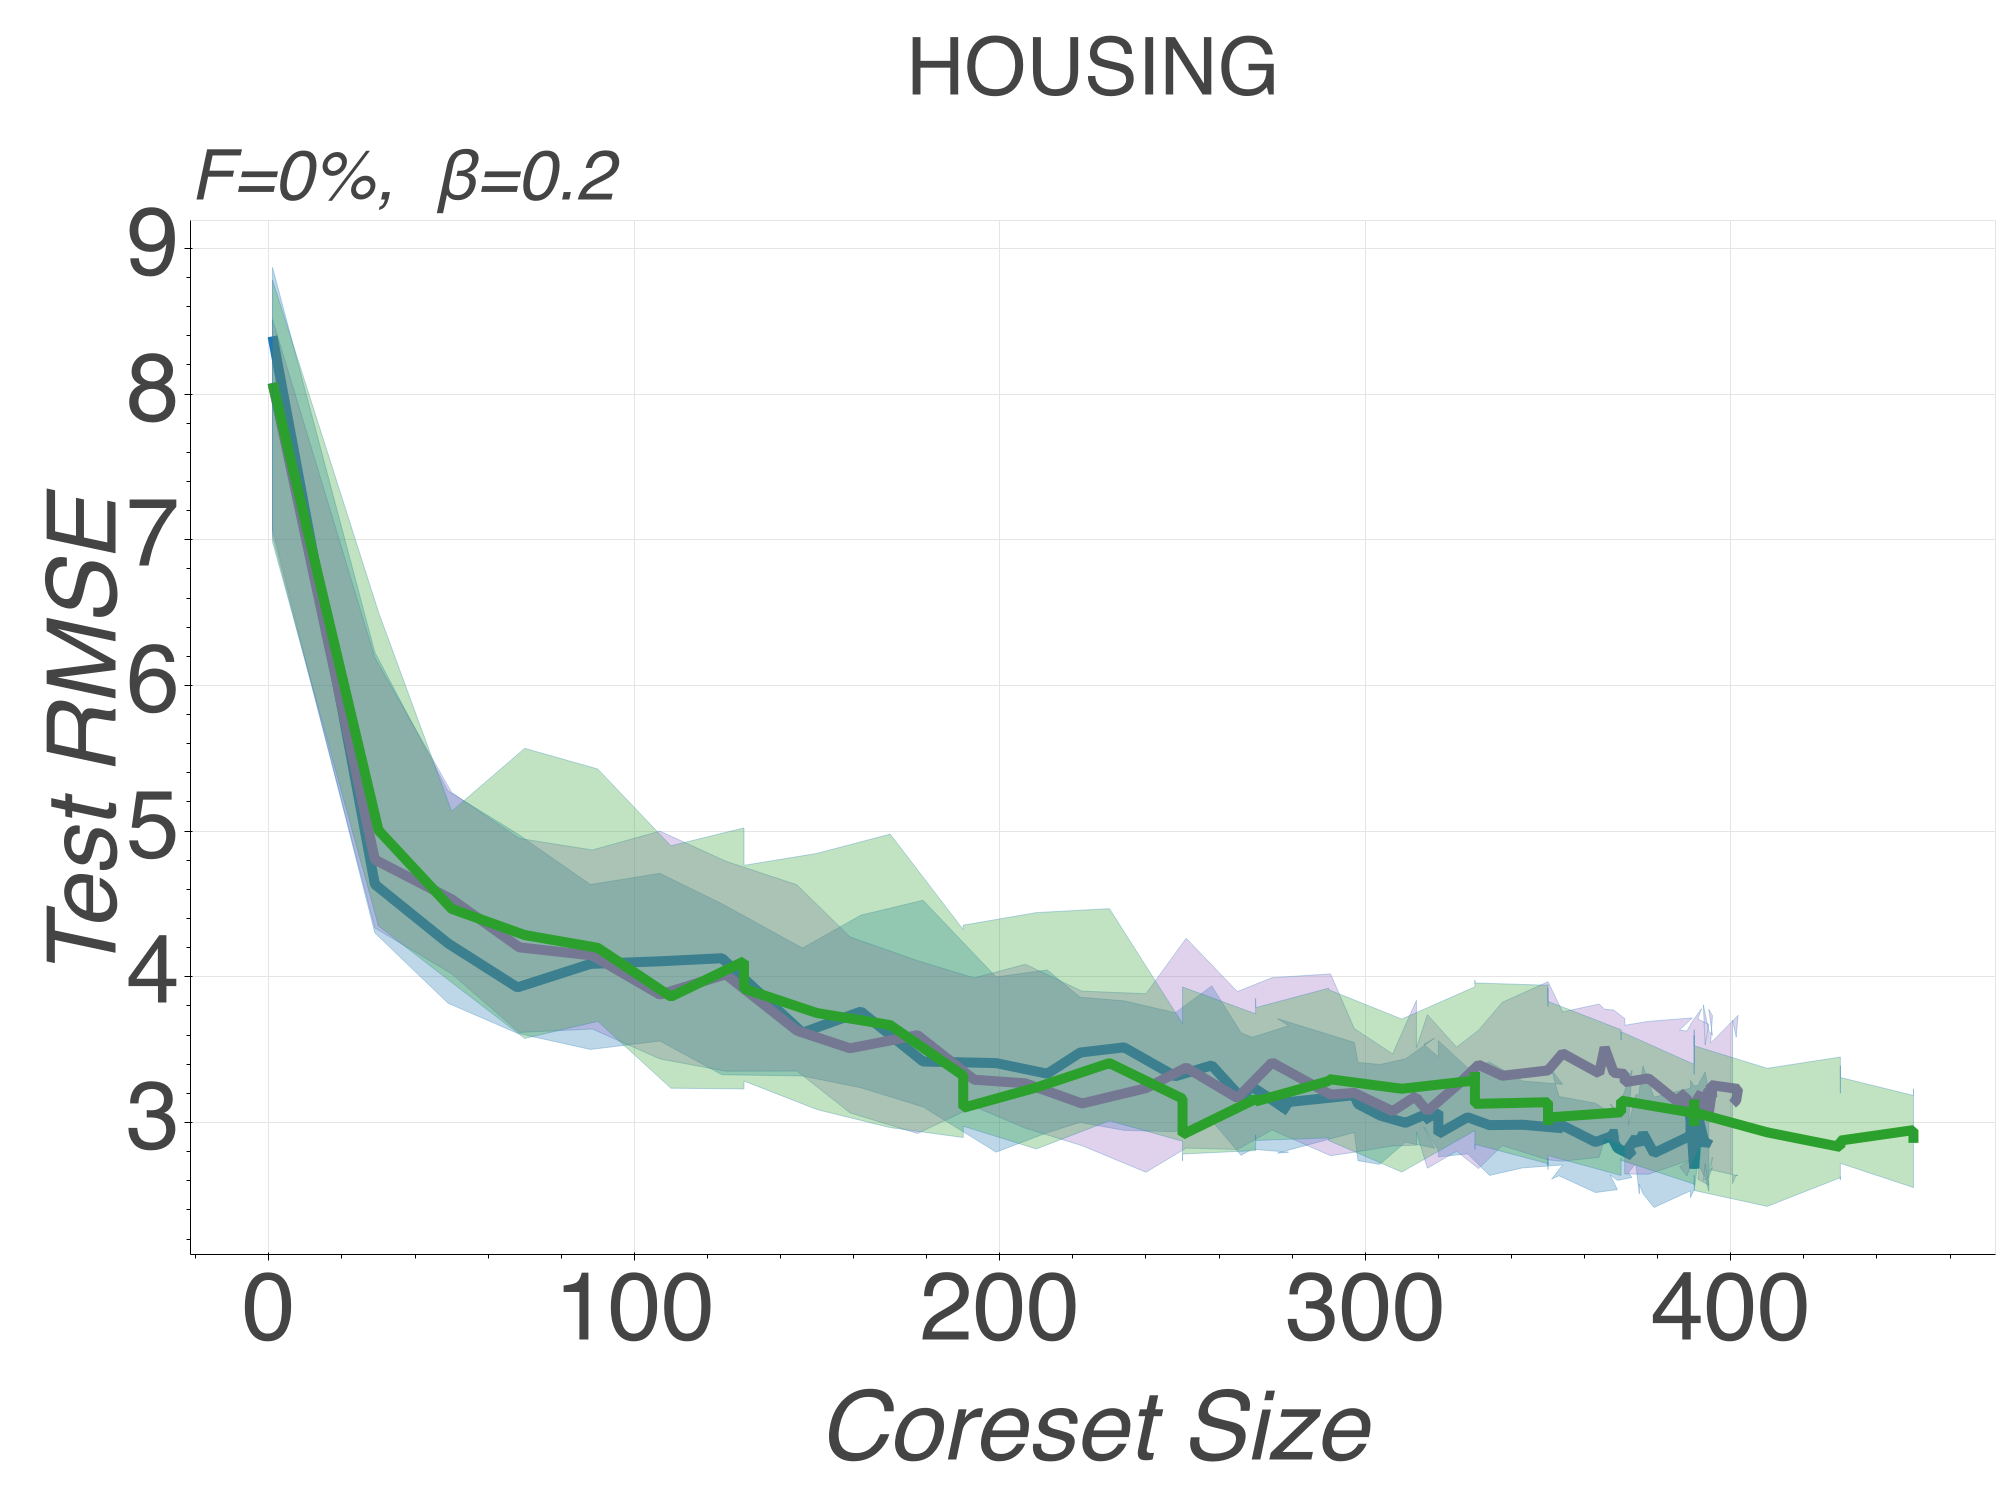
\includegraphics[width=.47\textwidth]{\MyPath/figs/boston02_01_0_RMSEvssz.png}
		\centering
		\hfill
		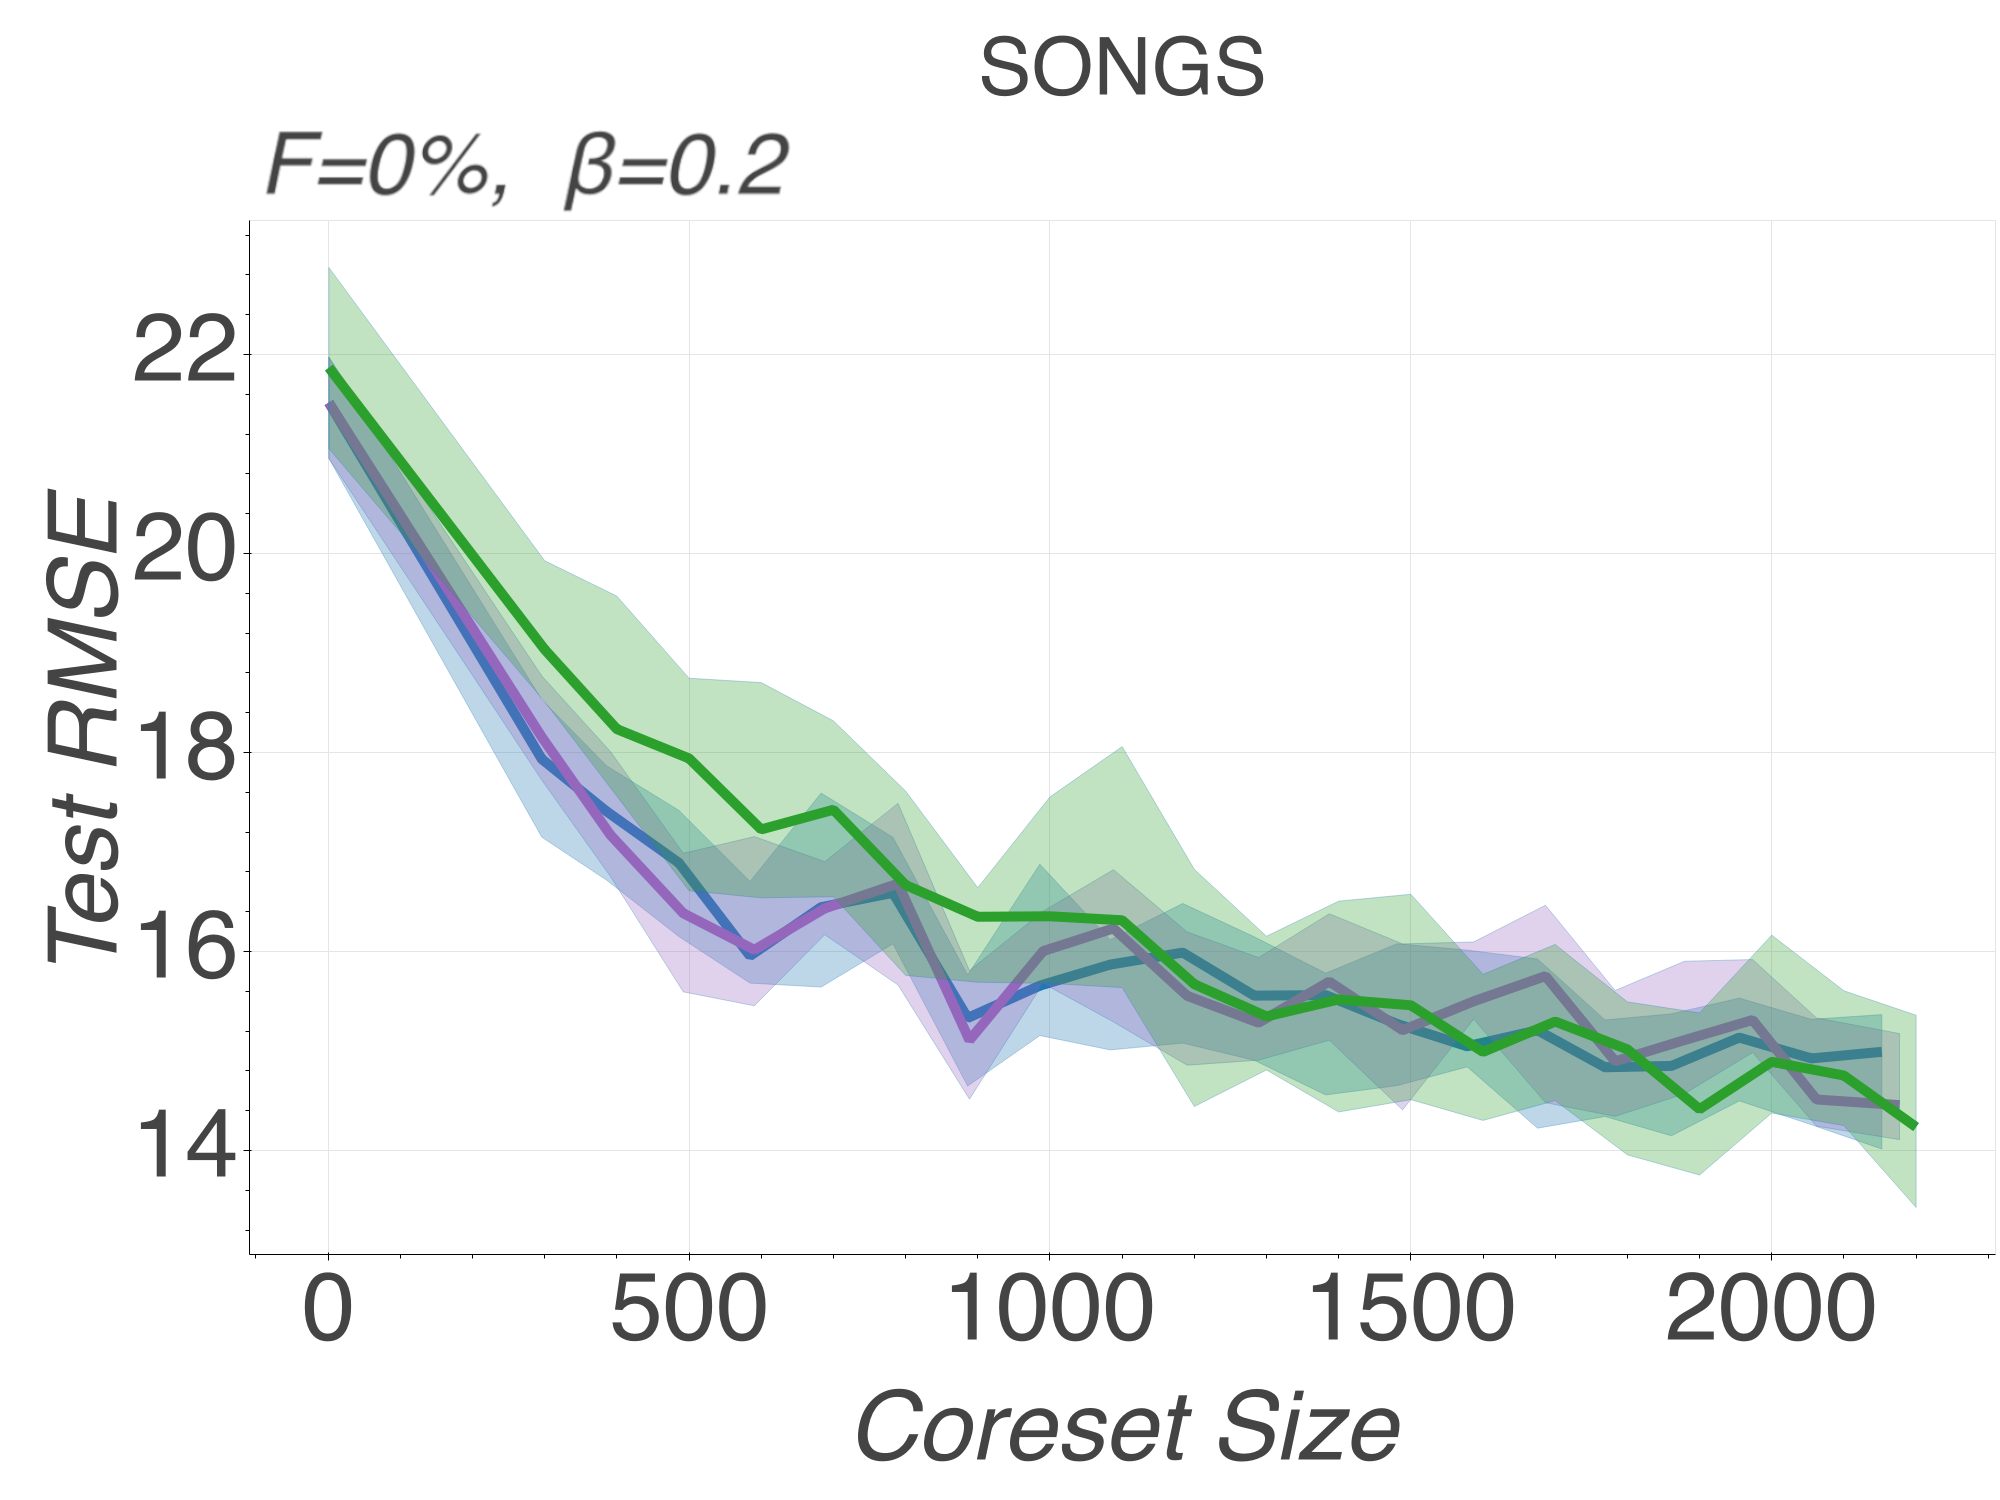
\includegraphics[width=.47\textwidth]{\MyPath/figs/year02_01_0_RMSEvssz.png}
	\end{subfigure}	
	\centering
	\caption{Test RMSE vs coreset size for neural linear regression experiments averaged over 30 trials. Solid lines display the median RMSE, with shaded areas showing $25\textsuperscript{th}$ and $75\textsuperscript{th}$ percentiles. Dataset corruption rate $F$, and $\beta$ value used in \bcores{} for each experiment are shown on the figures. The bottom row plots illustrate the achieved predictive performance under no contamination.}
	\label{fig:neural_plot}
\end{figure*}

We evaluate \bcores, \sparsevi{} and random sampling on two benchmark regression datasets~(detailed in~\cref{sec:data-details}). All coresets are initialized to a small batch of datapoints sampled uniformly at random from the dataset inliers. Over incremental construction, we interleave each minibatch selection and weights optimization step of the coreset with a training round for the neural network, constrained on the current coreset datapoints. Each such training round consists of $10^3$ minibatch gradient descent steps using the AdaGrad optimizer~\citep{mcmahan10,duchi10,duchi11}.
Our neural architecture is comprised of two fully connected hidden layers, batch normalization and ReLU activation functions. The values of coreset size at initialization, batch size added per coreset iteration, and units at each neural network hidden layer are set respectively to 20, 10 and 30 for the~\textsc{Housing}, and 200, 100 and 100 for the~\textsc{Songs} dataset.


\cref{fig:neural_plot}~(bottom row) shows that \bcores{} are competitive with the baselines in the absence of data corruption, achieving similar predictive performance over the entire range of tested coreset sizes. Under data poisoning~(top row), \bcores{} is the only method that offers monotonic decrease of test RMSE for increasing summary size from the beginning of the experiment. On the other hand, baselines present unreliable predictive performance for small coreset sizes: random sampling and \sparsevi{} are both prone to including corrupted data batches, whose misguiding information gets expressed on the flexible representations learnt by the neural network, requiring a larger summary size to reach the RMSE of \bcores.




\subsection{Efficient data acquisition from subpopulations for budgeted inference}
\label{sec:active-selection}


We consider the scenario where a machine learning service provider aims to fit a binary classification model to observations coming from multiple subpopulations of data contributors. The provider aims to maximize the predictive accuracy of the model, while adhering to a budget on the total number of subpopulations from which data can be accessed over inference. Budgeted inference can be motivated by several practical considerations: First, restricting the total number of datapoints used over learning to a smaller informative subset aids scalability---which is the primary motivation for coresets. Moreover, taking decisions at the subpopulations' level regarding which groups of datapoints are useful for the task, without the need to inspect datapoints individually, reduces the privacy loss incurred over the data selection stage, and can be integrated in machine learning pipelines that follow formal hierarchical privacy schemes~\citep{balle19}. Finally, subpopulations' valuation can guide costly experimental procedures, via inducing knowledge regarding which group combinations are most beneficial in summarizing the entire population of interest~\citep{pinsler19, vahidian20}, and hence should be prioritised over data collection.

In this study we use a subset of more than $60K$ datapoints from the \textsc{HospitalReadmissions} dataset (for further details see \cref{sec:data-details}). Using combinations of age, race and gender information of data contributors, we form a total of $165$ subpopulations within the training dataset. Data contamination is simulated identically to the experiment of \cref{subsec:logreg-expt}, while now we also consider the case of varying levels of contamination across the subpopulations. In particular, we form groups of roughly equal size where $0\%, 10\%$ and $20\%$ of the datapoints get replaced by outliers---this results in getting a dataset with approximately $10\%$ of its full set of datapoints corresponding to outliers.


\begin{figure*}[!t]
	\begin{subfigure}[b]{0.99\textwidth} 
		\centering
		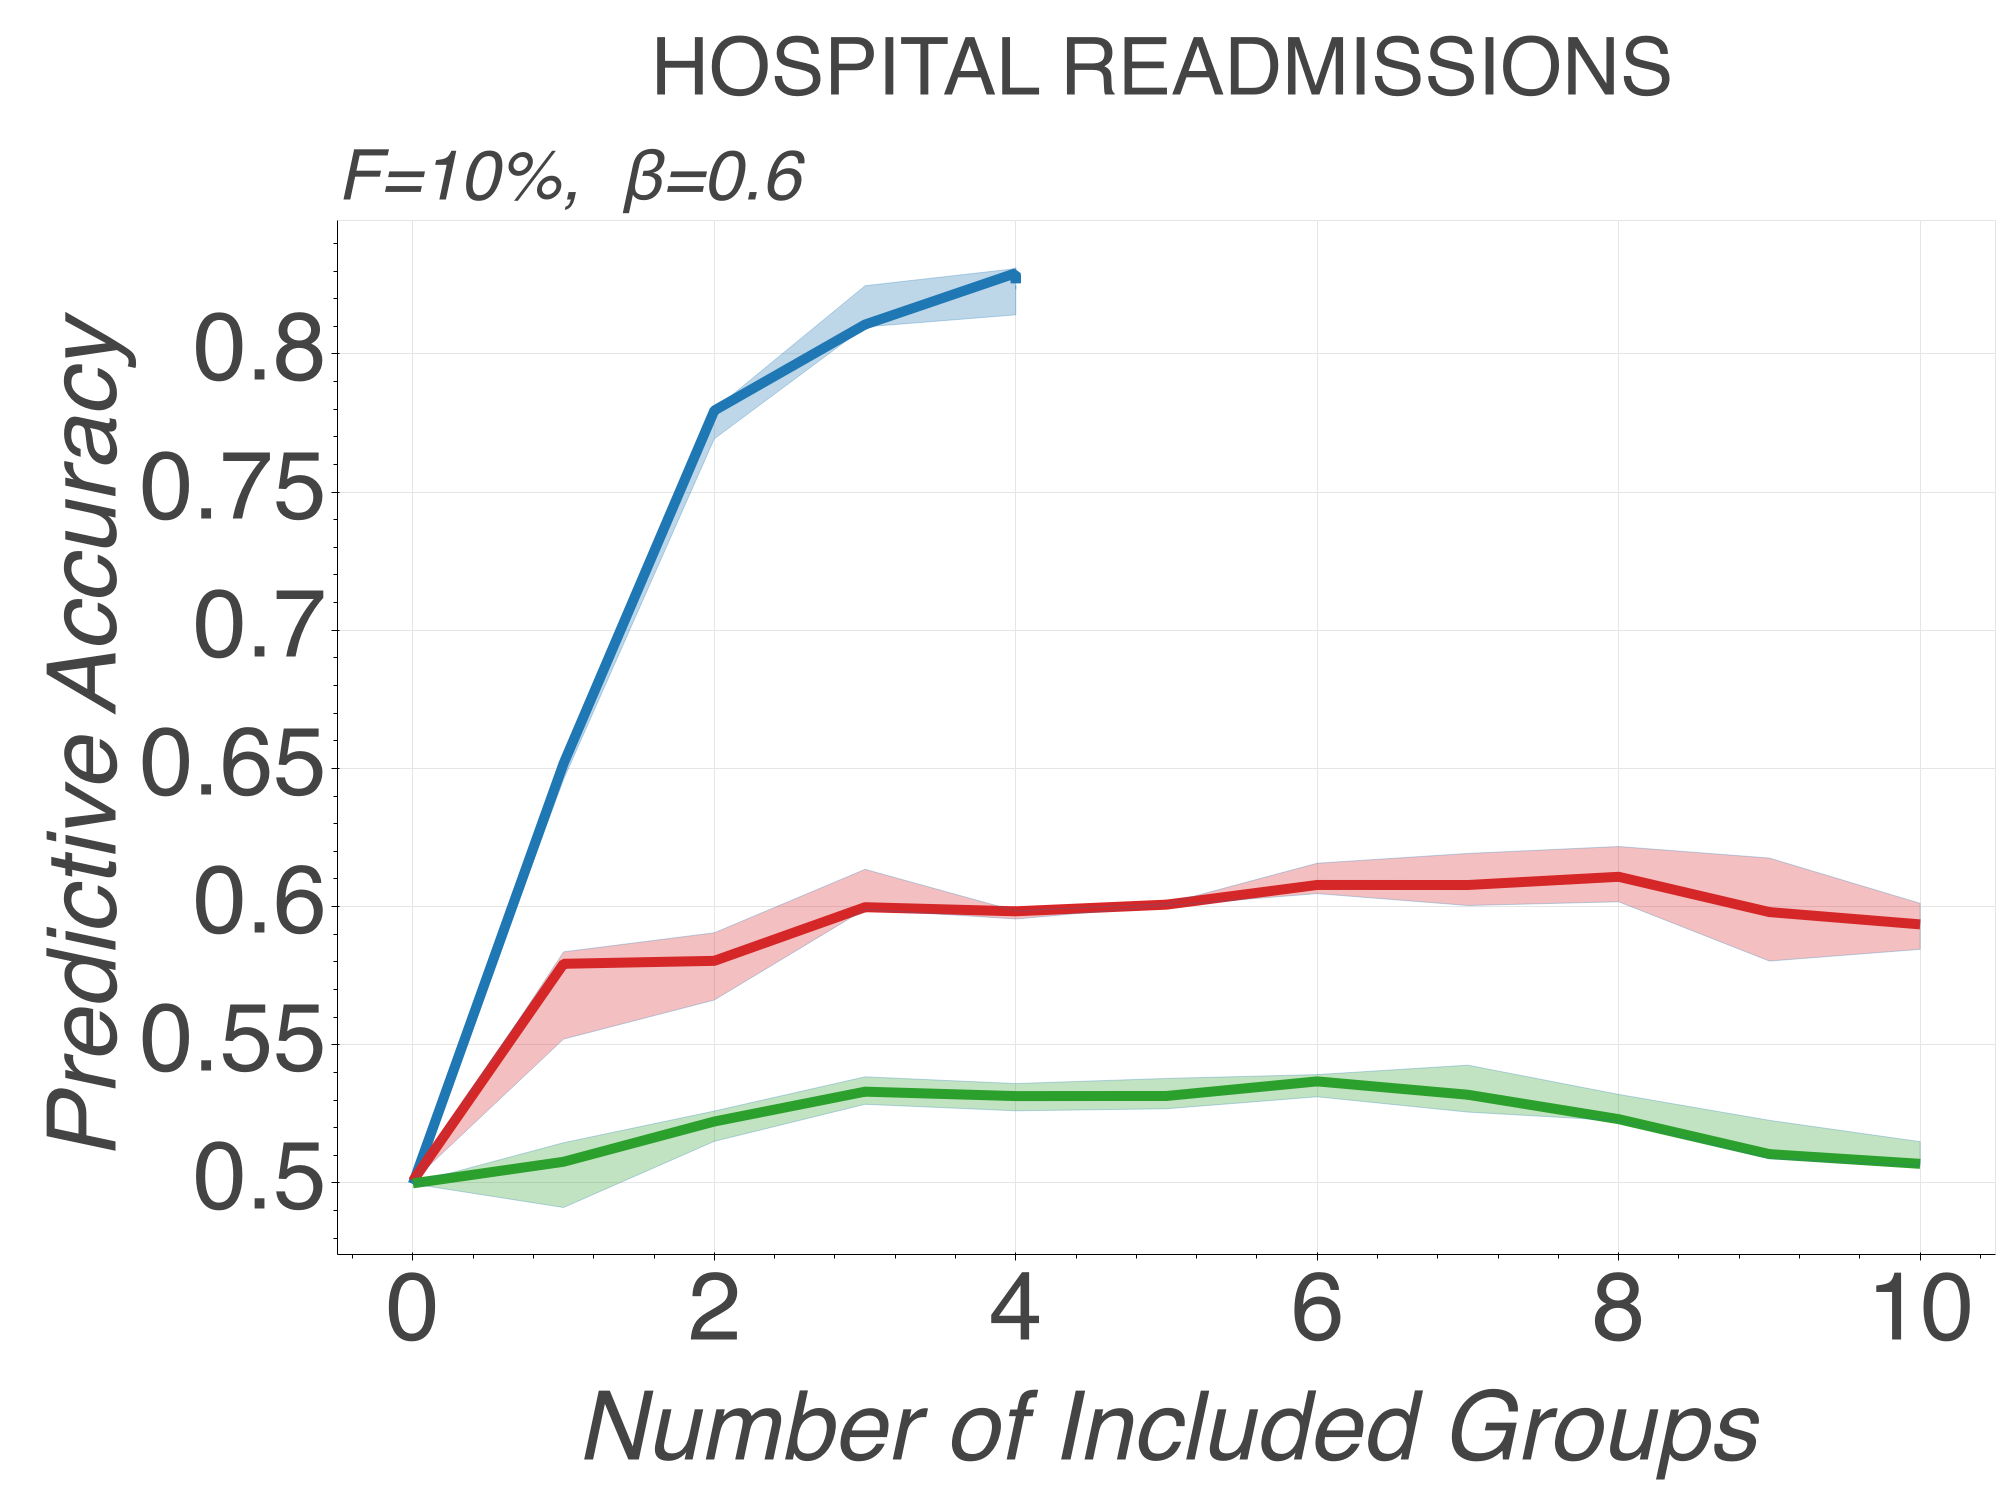
\includegraphics[width=.47\textwidth]{\MyPath/figs/group_diabetes06_10_01_False_ACCvsit.png}
		\hfill
		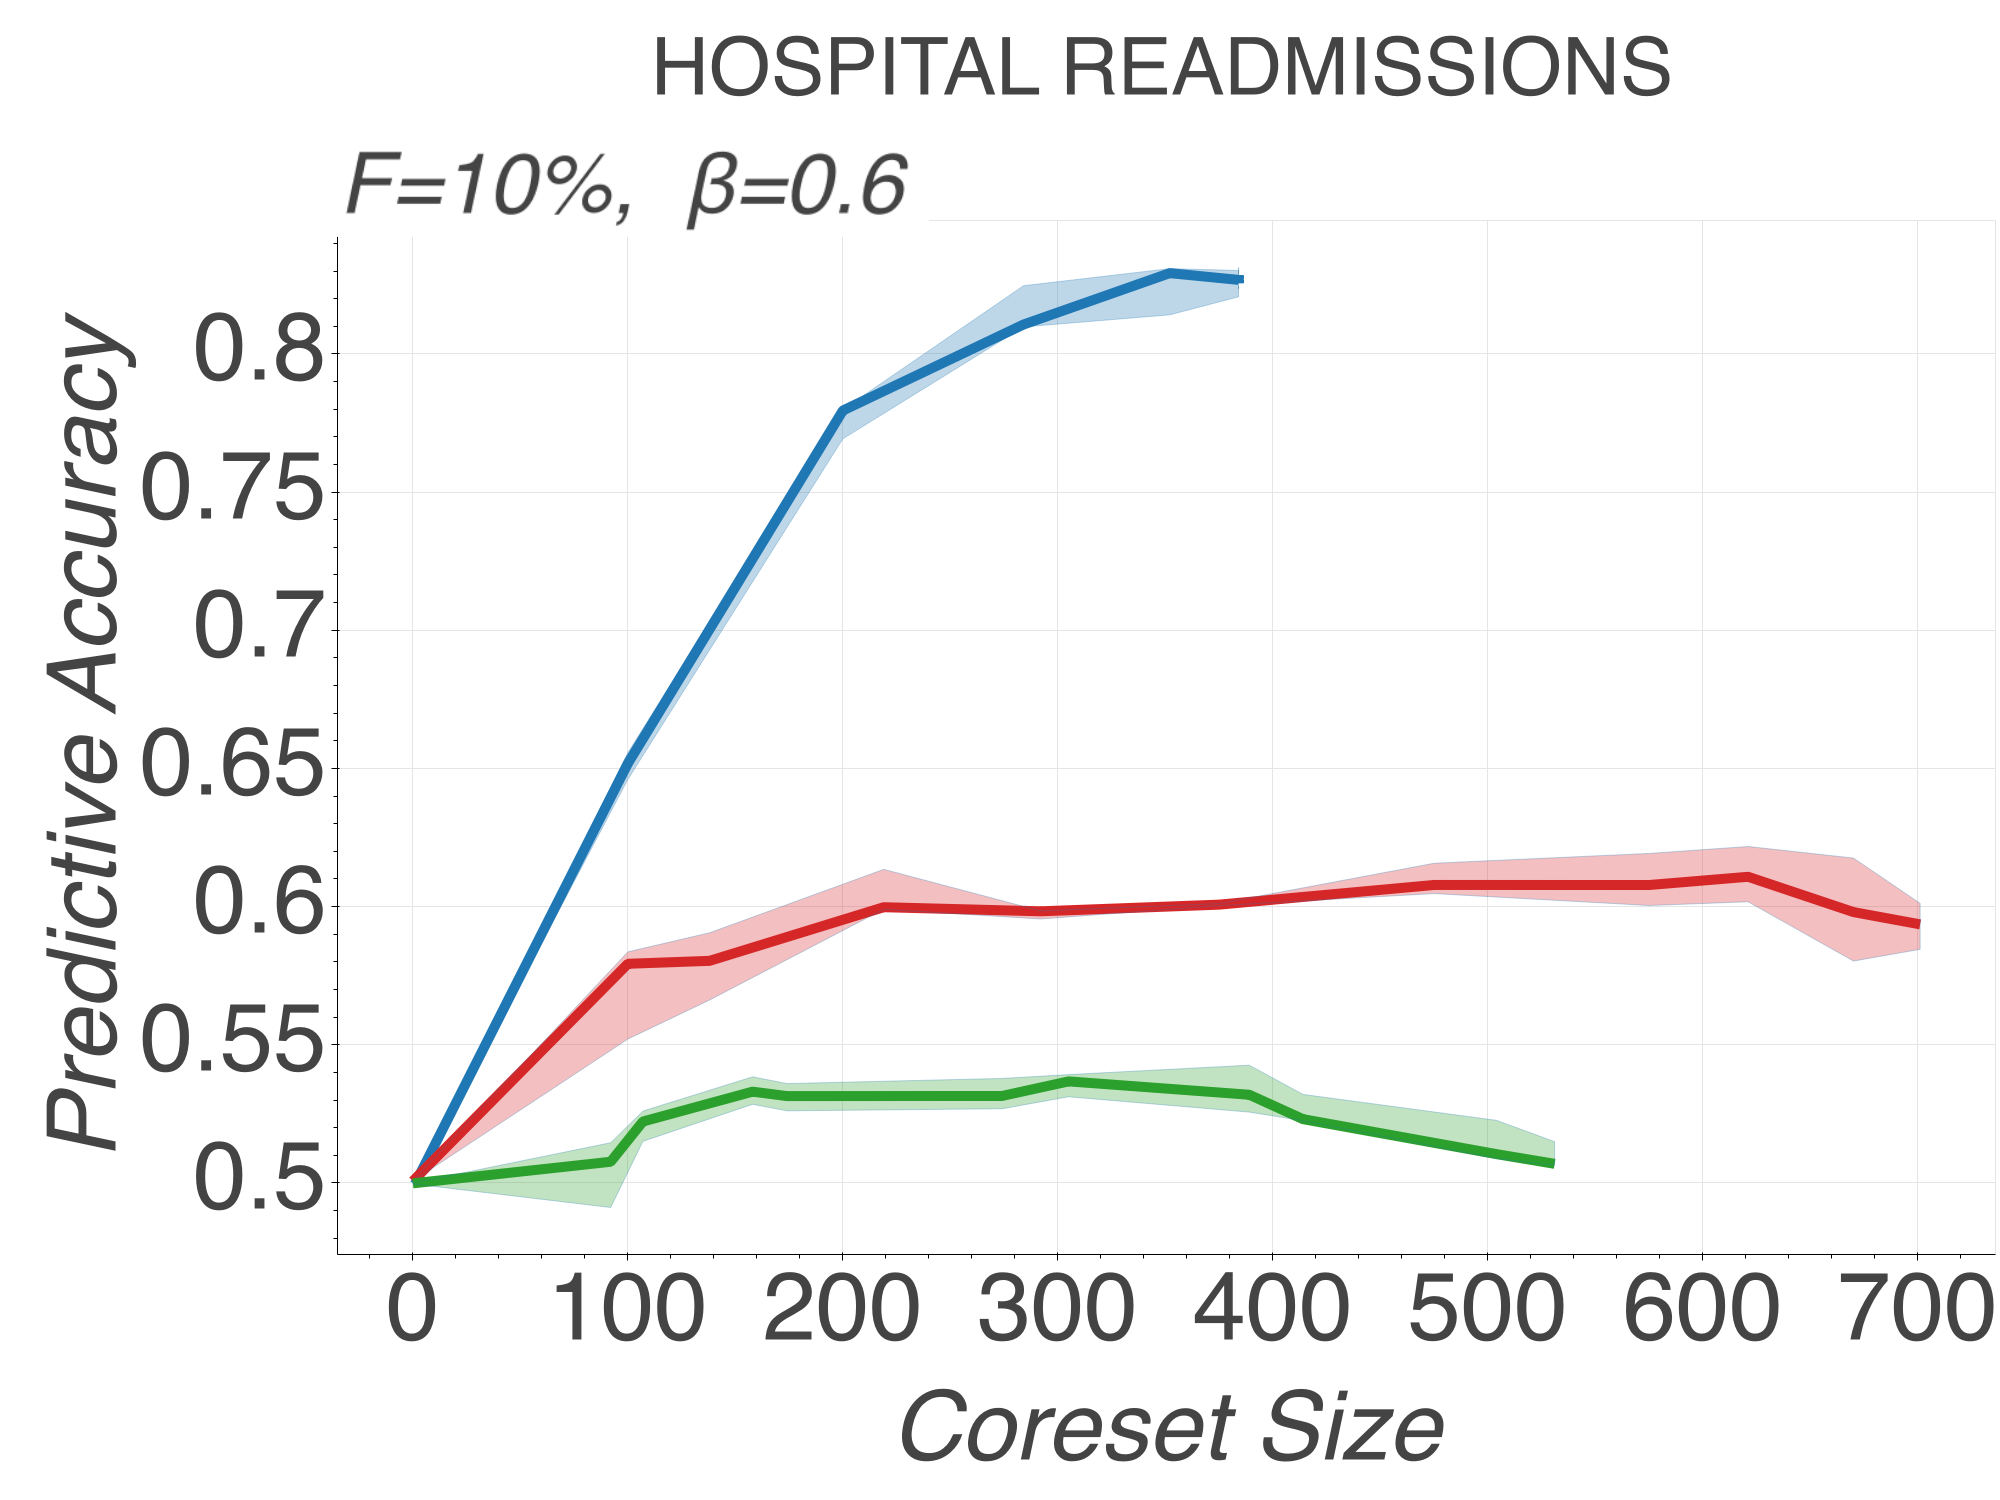
\includegraphics[width=.47\textwidth]{\MyPath/figs/group_diabetes06_10_01_False_ACCvssz.png}
		\centering
		\hfill
		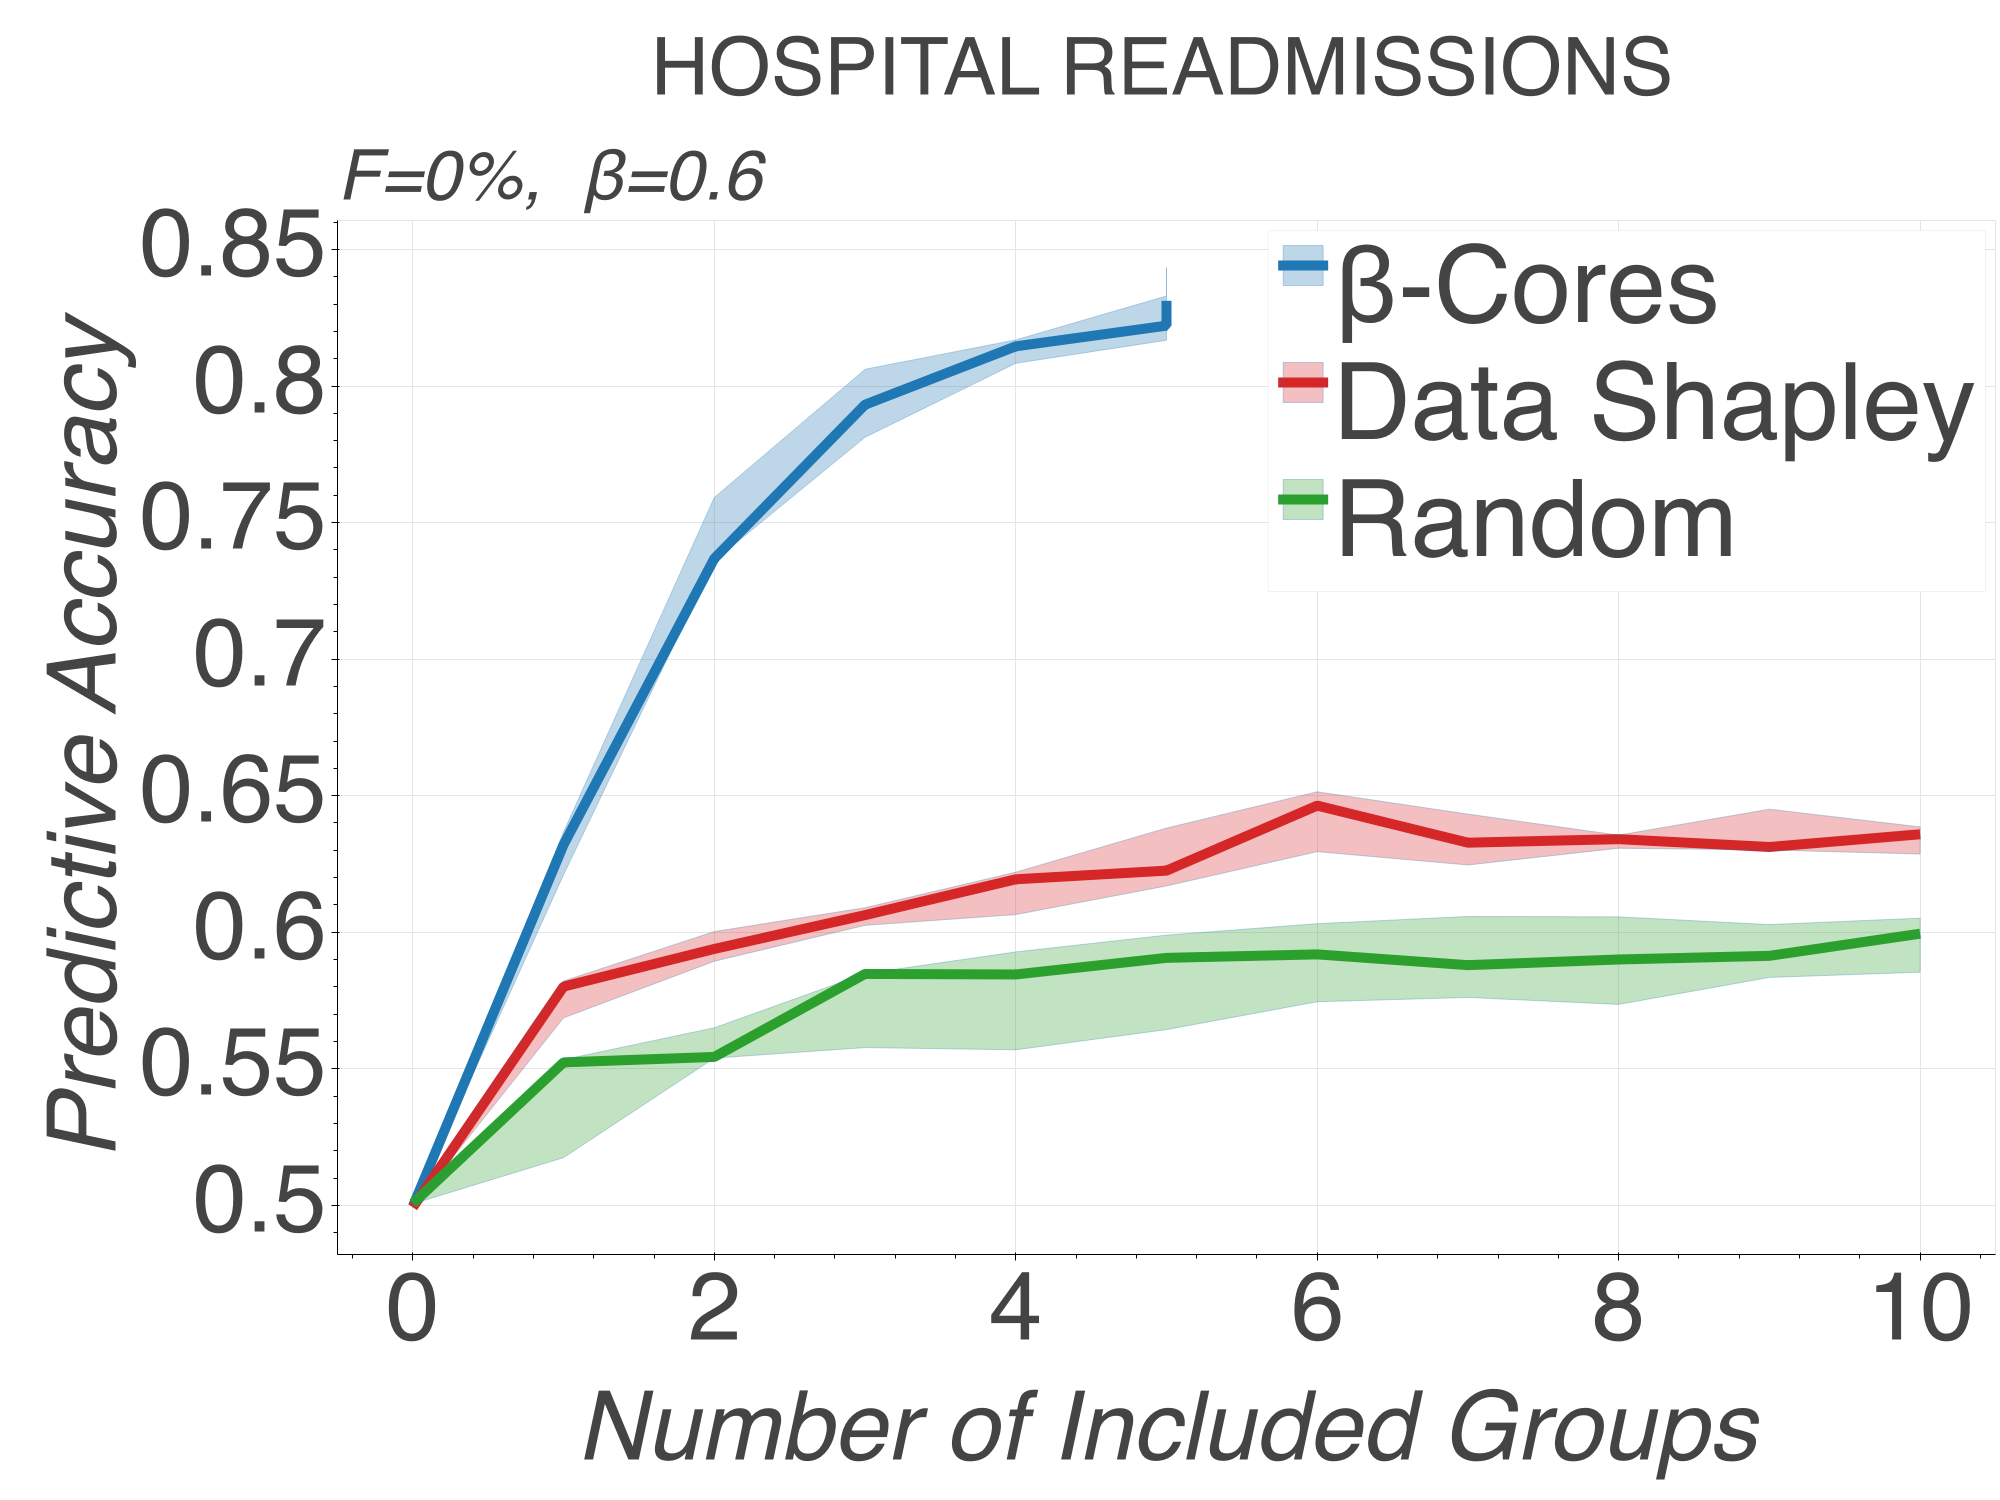
\includegraphics[width=.47\textwidth]{\MyPath/figs/group_diabetes06_10_0_False_ACCvsit.png}
		\centering
		\hfill
		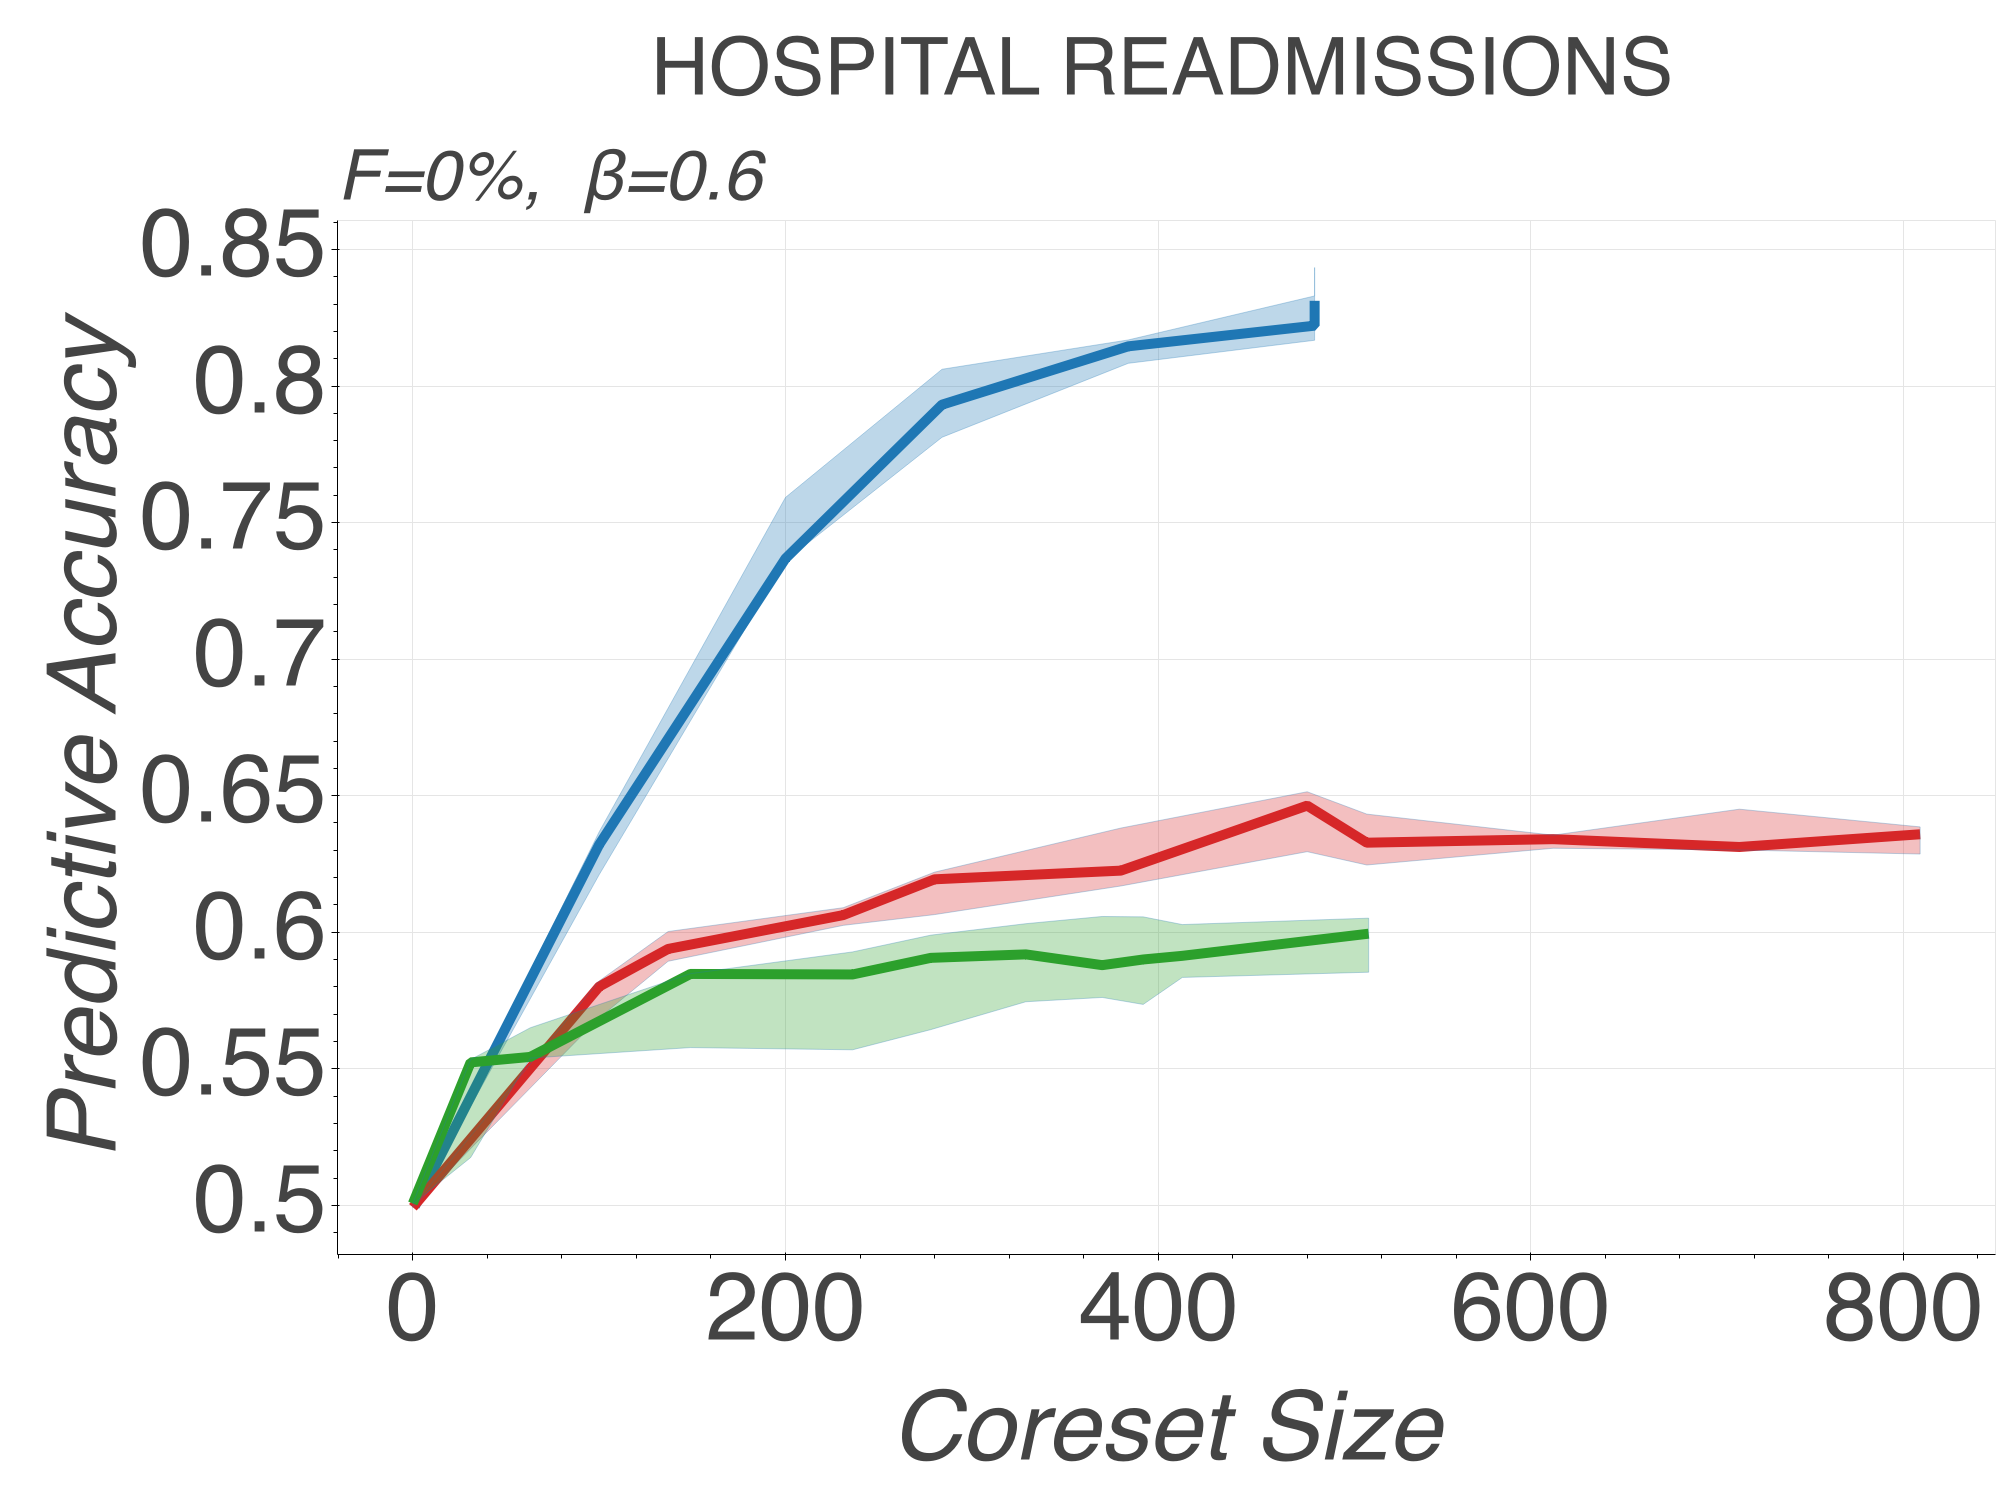
\includegraphics[width=.47\textwidth]{\MyPath/figs/group_diabetes06_10_0_False_ACCvssz.png}
	\end{subfigure}	
	\centering
	\caption{Predictive accuracy against number of groups~(left) and number of datapoints~(right) selected for inference. Compared group selection shemes are \bcores{}, selection according to Shapley values based ranking, and random selection. The experiment is repeated over $5$ trials, on a contaminated dataset containing a $10\%$ of crafted outliers distributed non-uniformly across groups~(top row), and a clean dataset~(bottom row).}
	\label{fig:group_plot}
\end{figure*}


We evaluate the predictive accuracy achieved by doing inference on the data subset obtained after running $10$ iterations of the \bcores{} extension for groups (which gives a maximum of $10$ selected groups). We compare against (\emph{i}) a \emph{random sampler}, and (\emph{ii}) a baseline which ranks all groups according to their \emph{Shapley value} and selects the groups with the highest ranks. Shapley value is a concept originating in cooperative game theory~\citep{shapley53}, which has recently found applications in data valuation and outliers detection~\citep{ghorbani19}. In the context of our experiment, it quantifies what is the marginal contribution of each group to the predictive accuracy of the model at all possible group coalitions that can be formed. As this quantity is notoriously expensive to be computed in large datasets, we use a Monte Carlo estimator which samples $5K$ possible permutations of groups and for each permutation it computes marginals for coalitions formed by the first $20$ groups.\footnote{The latter truncation is supported by the observation that marginal contributions to the predictive accuracy are diminishing as the dataset size increases.}

\begin{figure*}[!t]
	\begin{subfigure}[b]{.8\textwidth} 
		\centering
		\hspace*{2cm}
		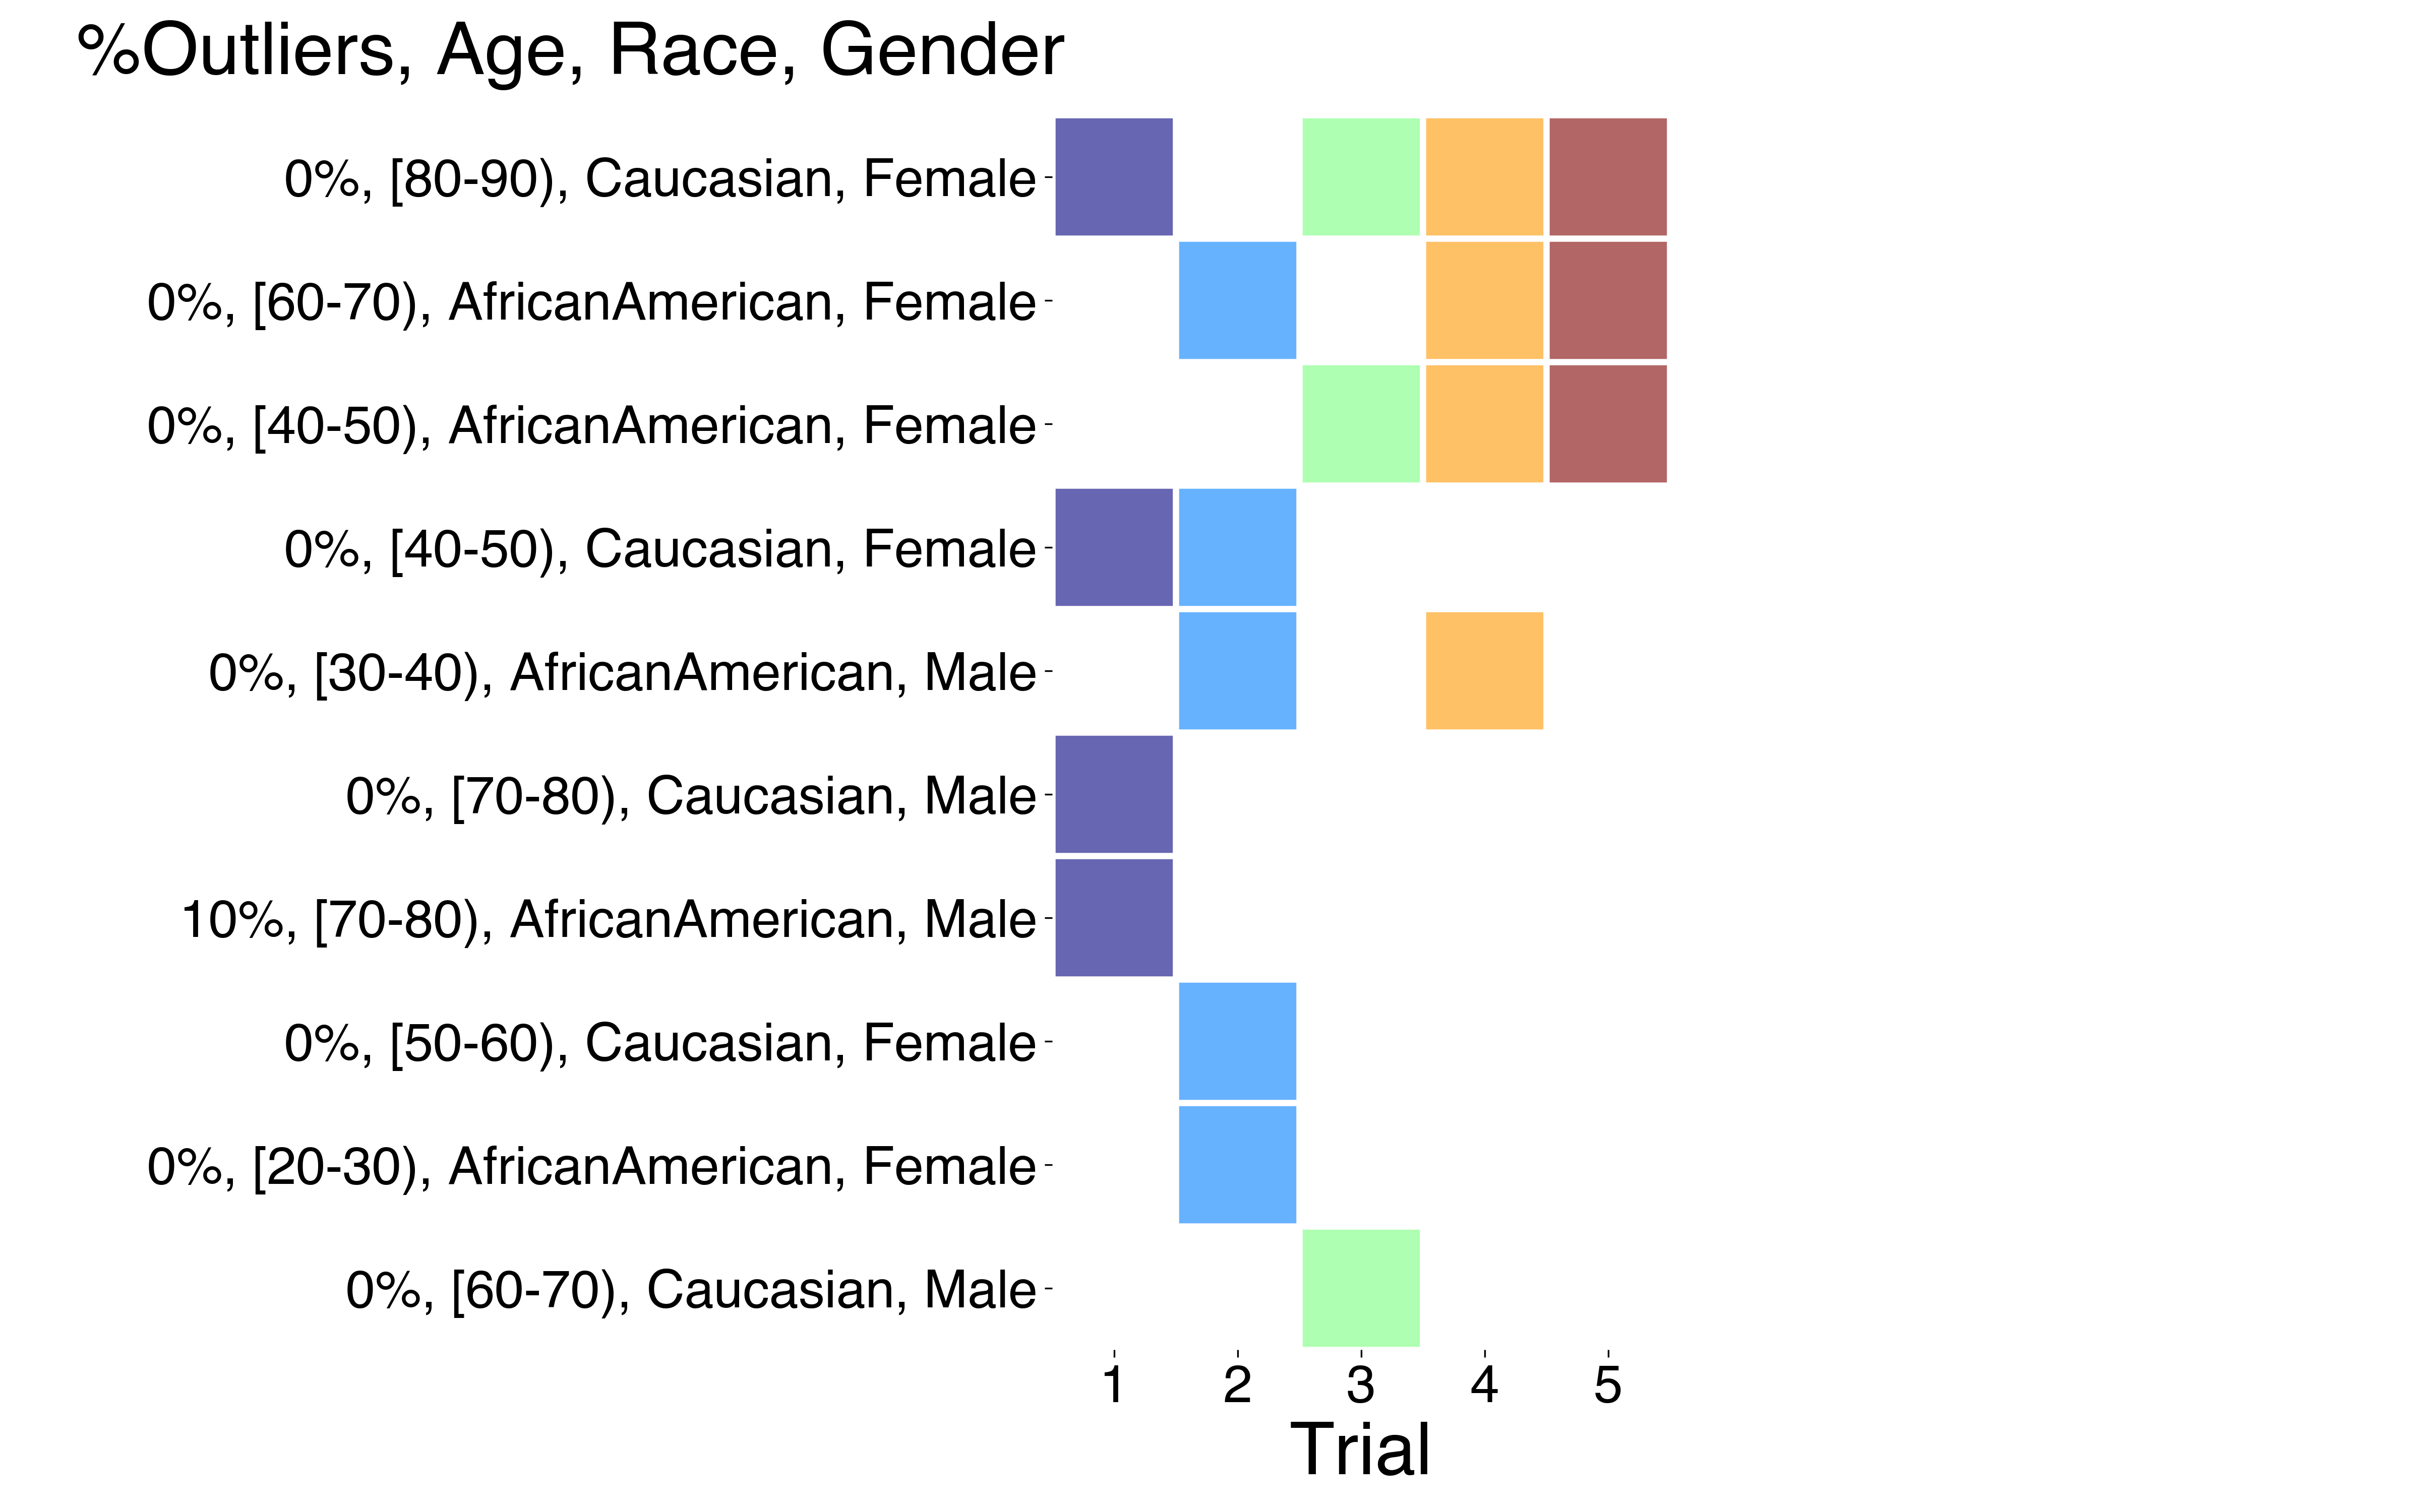
\includegraphics[width=.9\textwidth]{\MyPath/figs/selected_groups.png}
	\end{subfigure}	
	\centering
	\caption{Attributes of selected groups after running $10$ iterations of \bcores{} with $\beta=0.6$ on the contaminated \textsc{HospitalReadmissions} dataset (repeated over $5$ random trials).}
	\label{fig:selected_groups}
\end{figure*}

As illustrated in~\cref{fig:group_plot}, \bcores{} with $\beta=0.6$ offers the best solution to our problem, and is able to reach predictive accuracy exceeding $75\%$ by fitting a coreset on no more than $2$ groups. ~\cref{fig:selected_groups} displays the demographic information of selected groups. We can notice that subpopulations of female and older patients are more informative for the classification task, while Caucasian and African-American groups are preferred to smaller racial minorities. Importantly, \bcores{} is able to distill clean from contaminated groups. For the used $\beta$ value, we can see than over the set of trials only one group with outliers level of $10\%$ is allowed to enter a summary, which already contains $3$ uncontaminated groups.

Shapley values based ranking treats outliers better than random sampling: As outliers are expected to have negative marginal contribution to predictive accuracy, their Shapley rank is generally lower compared to clean data groups, hence the later are favoured. On the other hand, Shapley computation is much slower than random sampling and \bcores, specific to the evaluation metric of interest, while Shapley values are not designed to find data-efficient combinations of groups, hence this baseline can still retain redundancy in the selected data subset.




%\subsection{Case Study I: Regression on  Crowd-sourced Data under Labeling Noise}
%\label{subsec:logreg-expt}

%--- groups contributions and comparison to group shapley



%\subsection{Case Study III: Non-Negative Factorization of Users Implicit Feedback for Recommender Systems}
%\label{subsec:pmf-expt}
\section{Related Work}


\subsection{Mobility Deanonymization}

Protecting the anonymity of personal mobility is notoriously difficult due to sparsity~\citep{aggarwal2008} and hence mobility data are often vulnerable to deanonymization attacks~\citep{Narayanan2008}.
Numerous studies into location privacy have shown that even when an individual's data are anonymized, they continue to possess unique patterns that can be exploited by a malicious adversary with access to auxiliary information.
Zang et al.\ analysed nationwide call-data records (\emph{CDR}s) and showed that the $N$ most frequently visited places, so called \emph{top$-N$} data, correlated with publicly released side information and resulted in privacy risks, even for small values of $N$s~\citep{Zang2011}.
This finding underlines the need for reductions in spatial or temporal data fidelity before publication.
De Montjoye et al. quantified the unicity of human mobility on a mobile phone dataset of approximately $1.5M$ users with intrinsic temporal resolution of one hour and a 15-month measurement period~\citep{DeMontjoye2013}.
They found that four random spatio-temporal points suffice to uniquely identify $ 95\% $ of the traces.
They also observe that the uniqueness of traces decreases as a power law of spatio-temporal granularity, stressing the hardness of achieving privacy via obfuscation of time and space information.

Several inference attacks on longitudinal mobility are based on probabilistic models trained on individual traces and rely on the regularity of human mobility.
Mulder et al.\ developed a re-identification technique by building a Markov model for each individual in the training set, and then using this to re-identify individuals in the test set by likelihood maximisation~\cite{deMulder08}.
Similarly, Gambs et al.\ used Markov chains to model mobility traces in support of re-identification~\cite{Gambs2014}.

Naini et al.\ explored the privacy impact of releasing statistics of individuals mobility traces in the form of histograms, instead of their actual location information~\cite{Naini2016a}. They demonstrated that even this statistical information suffices to successfully recover the identity of individuals in datasets of few hundred people, via jointly matching labeled and unlabeled histograms of a population.
Other researchers have investigated the privacy threats from information sharing on location-based social networks, including the impact of location semantics on the difficulty of re-identification~\cite{privacyAndTheCity} and location inference~\cite{Agir}.

All the above previous work assumes locations are expressed using a universal symbol or global identifier, either corresponding to (potentially obfuscated) geographic coordinates, or pseudonymous stay points.
Hence, cross-referencing between individuals in the population is possible.
This is inapplicable when location information is anonymised separately for each individual.
Lin et al.\ presented a user verification method in this setting~\cite{LinMobile}.
It is based on statistical profiles of individual indoor and outdoor mobility, including cell tower ID and WiFi access point information.
In contrast, we employ network representations based solely on cell tower ID sequences without explicit time information.

Often, studies in human mobility aim to model properties of a population, thus location data are published as aggregate statistics computed over the locations of individuals.
This has traditionally been considered a secure way to obfuscate the sensitive information contained in individual location data, especially when released aggregates conform to $ k-$anonymity~\cite{sweeney2002k} principles.
However, recent results have questioned this assumption.
Xu et al.\ recovered movement trajectories of individuals with accuracy levels of between $73\%$ and $91\%$ from aggregate location information computed from cellular location information involving $100\,000$ users~\cite{xu2017trajectory}. Similarly, Pyrgelis et al.\ performed a set of inference attacks on aggregate location time-series data and detected serious privacy loss, even when individual data are perturbed by differential privacy mechanisms before aggregation~\cite{pyrgelis2017does}.

\subsection{Anonymity of Graph Data }
Most of the aforementioned data can be represented as \emph{microdata} with rows of fixed dimensionality in a table.
Microdata can thus be embedded into a vector space.
In other applications, datapoints are \emph{relational} and can be naturally represented as \emph{graphs}.
Measuring the similarity of such data is significantly more challenging, since there is no definitive method.
Deanonymization attacks on graphs have mostly been studied in the context of social networks and aimed to either align nodes between an auxiliary and an unknown targeted graph~\cite{narayanan2009anonymizing, sharad2014}, or quantify the leakage of private information of a graph node via its neighbors~\cite{zheleva09}.

In the problem studied here, \emph{each individual's information is an entire graph}, rather than a node in a graph or a node attribute, and thus deanonymization is reduced to a graph matching or classification problem.
To the best of our knowledge, this is the first attempt to deanonymize an individual's structured data by applying graph similarity metrics.
Since we are looking at relational data, not microdata, standard theoretical results on microdata anonymization, such as differential privacy \cite{dwork2006calibrating}, are not directly applicable.
However, metrics related to structural similiarity, including $k-$anonymity, can be generalized in this framework.

\section{Summary}% \& further directions}
\label{sec:conclusion}
In this chapter, we proposed a general purpose framework for yielding  contamination-robust summarizations of massive scale datasets for inference. Relying on recent advances in Bayesian coresets and robustified inference under the \bdiv{}, we developed a greedy black-box construction that efficiently shrinks big data via keeping informative datapoints, while simultaneously rejecting outliers.
 Finally, we presented experiments involving various statistical models, and simulated and real-world datasets, demonstrating that our methodology outperforms existing techniques in scenarios of structured and unstructured data corruption. 

Our future work will be concerned with considering stronger adversarial settings where summaries are initialized to data subsets that already contain outliers. Further directions also include automating the tuning of the robustness hyperparameter $\beta$, as well as applying our techniques to more complicated statistical models, including ones with structured likelihood functions (e.g. time-series and temporal point processes).
\input{acknowledgements}
\appendix
%\section{Gradient derivations}
\label{sec:gradient-derivations}
For brevity we suppress explicit indexing for moments under coreset posterior appearing below.
The gradient of the objective in~\cref{eq:sparsevi-obj} wrt to $w$, is written as
\[
\nabla_{w} \kl{\pi_{\beta,w}}{\pi} = &  \nabla_{w} \log Z(\beta, w) \\
													   & - \nabla_w \EE\left[1^Tf'(\theta)\right] + \nabla_w \EE\left[w^Tf(\theta)\right].
\label{eq:full-gradient}
\]
Using the known identity for the gradient of the log-parition function of an exponential family distribution~\citep{wainwright08}, the first term is reduced to
\[
\nabla_w \log Z(\beta, w) = \EE [f(\theta)].
\]
Via application of the product rule we get 
\[
\nabla_{w}\EE[w^Tf(\theta)] 
=& \int \nabla_w\left(\exp\left(w^T f(\theta) - \log Z(\beta, w)\right)\right)  w^T f(\theta) \pi_0(\theta) d\theta\\
  & -  \int \exp\left(w^T f(\theta) - \log Z(\beta, w)\right)  f(\theta) \pi_0(\theta) d\theta \\
=&\EE \left[ \left(f(\theta) - \nabla_w \log Z(\beta,w)\right) w^T f(\theta) \right] - \EE[f(\theta)]\\
=&\EE \left[ \left(f(\theta) - \EE [f(\theta)]\right) w^T f(\theta) \right] - \EE[f(\theta)].
\label{eq:dwfdw}
\]
Similarly
\[
\nabla_{w}\EE[1^Tf'(\theta)] 
=&\EE \left[ \left(f(\theta) - \EE [f(\theta)]\right) 1^T f'(\theta) \right].
\]
Substituting the derived expressions for all the terms in~\cref{eq:full-gradient}, subtracting 
\[0 =\EE \left[f(\theta) - \EE[f(\theta)] \right]\EE\left[ 1^T f'(\theta)\right] =\EE \left[f(\theta) - \EE[f(\theta)] \right]\EE\left[ w^T f(\theta)\right], 
\label{eq:subtract-trick}
\]
and using the (bi)linearity property of covariance, we get~\cref{eq:dkl-grad}. Computing an empirical estimate on a random minibatch of size $B$ is reduced to the approximation of~\cref{eq:gradw}.

The gradient of the objective in~\cref{eq:sparsevi-obj} wrt to $\beta$, is written as
\[
\nabla_\beta \kl{\pi_{\beta,w}}{\pi} = &  \nabla_\beta \log Z(\beta, w) \\
& - \nabla_\beta \EE\left[1^Tf'(\theta)\right] + \nabla_\beta \EE\left[w^Tf(\theta)\right].
\label{eq:full-gradient-beta}
\]
Recalling that $k(\cdot, \theta):=(\nabla_\beta f_n(\cdot, \theta))_{n=1}^{N}$, we get
\[
\nabla_\beta \log Z(\beta, w) = w^T\EE[k(\beta, \theta)].
\]
Following similar steps with~\cref{eq:dwfdw}, we derive
\[
\nabla_\beta \EE\left[w^Tf(\theta)\right] = w^T\EE\left[\left(k(\beta, \theta)-\EE\left[k(\beta, \theta)\right]\right)w^Tf(\theta)\right] + w^T\EE[k(\beta, \theta)],
\]
and
\[
\nabla_\beta \EE\left[1^Tf'(\theta)\right] = w^T\EE\left[\left(k(\beta, \theta)-\EE\left[k(\beta, \theta)\right]\right)1^Tf'(\theta)\right].
\]
Applying a subtraction trick for functions $k$ as in~\cref{eq:subtract-trick}, we 
eventually get
\[
\nabla_{\beta}\kl{\pi_{\beta,w}}{\pi} 
& = -w^T\cov_{\beta,w}\left[k(\beta),1^Tf' -w^Tf\right].
\label{eq:dkl-grad-beta}
\]


\section{Models}
\label{sec:models}
In this section we present the derivations of \blik{} terms~\cref{eq:b-loss,eq:sl-lik-terms} required over the \bcores{} constructions for the statistical models of our experiments.

\subsection{Gaussian likelihoods}
\label{sec:gauss-lik}

For the \blik{} terms of a multivariate normal distribution, we have 
\[
\pi(x|\mu, \Sigma)^{\beta} = \left((2\pi)^{-\frac{d}{2}}|\Sigma|^{-\frac{1}{2}}\right)^{\beta} \exp\left(-\frac{\beta}{2}(x-\mu)^T\Sigma^{-1}(x-\mu)\right),
\]
and, by simple calculus (see also~\citep{samek13}),
\[
\int_{\mcX}\pi(\chi|\mu, \Sigma)^{1+\beta}d\chi = \left((2\pi)^{-\frac{d}{2}}|\Sigma|^{-\frac{1}{2}}\right)^{\beta}(1+\beta)^{-\frac{d}{2}}.
\]
Hence
\[
f_n(\mu) 
 \propto &  \frac{1}{\beta}\left((2\pi)^{-\frac{d}{2}}|\Sigma|^{-\frac{1}{2}}\right)^{\beta} \exp\left(-\frac{\beta}{2}(x-\mu)^T\Sigma^{-1}(x-\mu)\right) \\
 &-\left((2\pi)^{-\frac{d}{2}}|\Sigma|^{-\frac{1}{2}}\right)^{\beta}(1+\beta)^{-\frac{d}{2}-1}\\
 \propto &
 \frac{1}{\beta} \exp\left(-\frac{\beta}{2}(x-\mu)^T\Sigma^{-1}(x-\mu)\right) 
 -(1+\beta)^{-\frac{d}{2}-1}
 \label{eq:gaussian-beta-lik}.
\]
\begin{comment}
and
\[
k_n(\mu) =& \left((2\pi)^{-\frac{d}{2}}|\Sigma|^{-\frac{1}{2}}\right)^{\beta}  
\times \left[\log\left((2\pi)^{-\frac{d}{2}}|\Sigma|^{-\frac{1}{2}}\right) \right. \\
&\left. \times \left( \frac{1}{\beta} \exp\left(-\frac{\beta}{2}(x-\mu)^T\Sigma^{-1}(x-\mu)\right) -(1+\beta)^{-\frac{d}{2}-1}\right) \right.
\\ &  \left. -  \frac{1}{\beta^2} \exp\left(-\frac{\beta}{2}(x-\mu)^T\Sigma^{-1}(x-\mu)\right) \right.
\\&- \left. \frac{1}{2\beta}  (x-\mu)^T\Sigma^{-1}(x-\mu)\exp\left(-\frac{\beta}{2}(x-\mu)^T\Sigma^{-1}(x-\mu)\right) \right.
\\& \left. - (1+\beta)^{-\frac{d}{2}-1} \log(1+\beta) \right]. 
 \label{eq:gaussian-grad-beta}
\]
\end{comment}

\subsection{Logistic regression likelihoods}
\label{sec:logreg-lik}
Log-likelihood terms of individual datapoints are given as follows
\[
\log \pi(y_n|x_n, \theta) = -\log\left(1+e^{-y_n z_n^T \theta}\right).
\label{eq:logreg-loglik}
\]
Substituting to~\cref{eq:sl-lik-terms}, for the  \blik{} terms we get
\[
f_n(\theta)& \propto -\frac{1}{\beta}\left(1+e^{-y_n z_n^T \theta}\right)^{-\beta} \\
&+ \frac{1}{\beta+1} \left( \left(1+e^{- z_n^T \theta}\right)^{-(\beta+1)} + \left(1+e^{z_n^T \theta}\right)^{-(\beta+1)} \right).
\label{eq:logreg-blik}
\]

\subsection{Neural linear regression likelihoods and predictive posterior}
\label{sec:neurlinr-lik}
Recall that in the neural linear regression model, $ \left(y_n - \theta^T z(x_n)\right) \sim \distNorm(0, \sigma^2), \; n=1,\ldots,N$. %for a generic deterministic feature extractor ${z(\cdot): \mcX \rightarrow \reals^{d}}$ learned from the data $(x,y):=\left( x_n, y_n\right)_{n=1}^{N}$. 
Then the Gaussian log-likelihoods corresponding to individual observations (after dropping normalization constants),  are written as 
\[
f_n(\theta) = - \frac{1}{2\sigma^2}\left(y_n - \theta^T z(x_n)\right)^2.
\label{eq:neurlinr-logliks}
\]
Assuming a prior $\theta \dist \distNorm(\mu_0, \sigma_0^2 I)$, the coreset posterior can be computed in closed form as follows
\[
\pi_w(\theta) = \distNorm\left(\mu_w, \Sigma_w\right),
\label{eq:neurlinr-coreset-posterior}
\]
where 
\[
&\Sigma_w := \left(\sigma_0^{-2}I + \sigma^{-2} \sum_{m=1}^{M}w_m z(x_m) z(x_m)^T \right)^{-1},\\
&\mu_w := \Sigma_w \left( \sigma_0^{-2} I \mu_0 + \sigma^{-2} \sum_{m=1}^{M} w_m y_m z(x_m) \right).
\label{eq:neurlinr-corest-posterior-params}
\]
By substitution to~\cref{eq:sl-lik-terms},
the \blik{} terms for our adaptive basis linear regression are written as 
\[
f_n(\theta) \propto  \frac{1}{(2\pi)^{\beta/2}\sigma^{\beta}} \left(-\frac{\beta+1}{\beta}e^{-\beta\left(y_n-\theta^Tz(x_n)\right)^2/(2\sigma^2)} + \frac{1}{\sqrt{1+\beta}}\right).
\label{eq:linreg-blik}
\]
%To simplify notation 
Let $\mcC$ be the output of the coreset applied on a dataset $\mcD$. Hence, in regression problems, the predictive posterior on a test data pair $(x_t, y_t)$ via a coreset is approximated as follows
\[
\pi(y_t|x_t, \mcD) & \approx \pi(y_t|x_t, \mcC)  \\
&= \int \pi(y_t|x_t,  \theta) \pi(\theta|\mcC) d\theta.  
\label{eq:coreset-postpred}
\]
In the neural linear experiment, 
the predictive posterior is a Gaussian given by the following formula
\[
\pi(y_t|x_t, \mcC) 
& = \distNorm \left(y_t; \mu_w^T z(x_t), \sigma^2 + z(x_t)^T \Sigma_w z(x_t)\right).
\label{eq:neurlinr-pred-posterior}
\]
%with $\mu_w, \Sigma_w$, defined as in~\cref{sec:neurlinr-lik}.


\begin{comment}
\subsection{Poisson likelihoods}
\label{sec:poisson-lik}

Our Poisson factorization model is defined as follows~\cite{cemgil09, gopalan15, wang17}
\[
&\phi_{uk} \distiid \distExp(10^{3}),  &(u,k) \in [U] \times [K],\\
& \psi_{ik} \distiid \distExp(10^{3}),  &(i,k) \in [I] \times [K],\\
& x_{ui} \sim \distPoiss(\phi_u^T\psi_i),  &(u,i) \in [U] \times[I].
\label{eq:pmf-model}
\]
Hence, the likelihood of a single observation and the log-likelihood over the full matrix of observations can be written as 
\[
p(x_{ui}|\phi_{u}, \psi_{i}) = (\phi_u^T \psi_i)^{x_{ui}} \exp\left(-\phi_u^T \psi_i\right)/x_{ui}!,
\label{eq:pmf-single-lik}
\]
and
\[
\log p(x|\phi, \psi) = \sum_{x_{ui}>0} \left(x_{ui} \log \left(\phi_u^T \psi_i\right) - \log \Gamma(x_{ui}+1)\right)  - (1^T\phi)(1^T \psi),
\label{eq:pmf-loglik}
\]
where $ \Gamma(s+1):=s! $ is the gamma function.

For the \blik-terms, we get
\[
t_{ui}(\phi_u, \psi_i) = \frac{1}{\beta} (\phi_u^T \psi_i)^{\beta x_{ui}}
\exp\left(-\beta \phi_u^T \psi_i\right)/\left(x_{ui}!\right)^\beta,
\label{eq:pmf-blik}
\]
and
\[
c(\phi_u, \psi_i)=-\frac{1}{\beta+1} \sum_{\chi \geq 0} \left((\phi_u^T \psi_i)^{\chi} \exp\left(-\phi_u^T \psi_i\right)/\chi!  \right)^{\beta+1}.
\]
The last term can be computed approximatelly by numerical evaluation of the rapidly converging infinite sum.
\end{comment}

\begin{comment}
\subsection{Coreset posterior predictive distributions}
\label{sec:pred-post}
To simplify notation let's denote by $\mcC$ the output of the coreset applied on a dataset $\mcD$. Hence, in regression problems, the posterior predictive on a test data pair $(x_t, y_t)$ via a coreset is approximated as follows
\[
\pi(y_t|x_t, \mcD)  \approx \pi(y_t|x_t, \mcC) 
&= \int \pi(y_t|x_t,  \theta) \pi(\theta|\mcC) d\theta.  
\label{eq:coreset-postpred}
\]

In the logistic regression experiment, presented results follow the MC approximation of the above (intractable) integral is
\[
\pi(y_t=1|x_t, \mcC) 
 \approx \frac{1}{S} \sum_{s=1}^{S} \frac{1}{1+\exp(\theta_s^T x_t)}, \qquad \theta_s \sim \pi(\theta| \mcC).
\label{eq:logreg-predpost-mc}
\]
\end{comment}


\section{Datasets Details}
\label{sec:data-details}

The benchmark datasets used in logistic regression (including group selection) and neural linear regression experiments are detailed in Tables~\ref{table:logreg-data} and \ref{table:neurlinreg-data} respectively.\footnote{The original versions of all used datasets can be accessed by following the corresponding hyperlinks in the Tables appearing in the electronic version of the thesis.}, and include: 
\begin{itemize}
\item a dataset used to predict whether a citizen's income exceeds $50K \$$ per year extracted from USA 1994 census data~(\textsc{Adult}),
\item a dataset containing webpages features and a label categorizing them as phishing or not~(\textsc{Phishing}),
\item a corpus of webpages crawled from links found in spam emails~(\textsc{WebSpam}),
\item a set of hospitalization records for binary prediction of readmission pertaining to diabetes patients~(\textsc{HospitalReadmissions}),
\item a set of various features from homes in the suburbs of Boston, Massachussets used to model housing price~(\textsc{Housing}), and
\item a dataset used to predict the release year of songs from associated audio features ~(\textsc{Songs}).
\end{itemize} 

For \textsc{Adult}, \textsc{Phishing} and \textsc{HospitalReadmissions} we fit our statistical models on the first 10 principal components of the datasets, while  all logistic regression benchmark datasets are evaluated on balanced subsets of the test data between the two classes~(see~\cref{table:logreg-data}).
	\begin{table}[!t]
		\caption{Logistic regression datasets}
		\centering
		\resizebox{0.85\columnwidth}{!}{%
		\begin{tabular}{lrrrrr}
			\hline
			Dataset      &   $d$ &     $N\textsubscript{train}$ &   $N\textsubscript{test}$ &   $\#$Pos. test data 
			 \\
			\hline
			\MYhref{http://archive.ics.uci.edu/ml/datasets/Adult}{\textsc{Adult}}~\citep{adult}        &  10 &  30,162 &    7,413 &             3,700  \\
			\MYhref{https://archive.ics.uci.edu/ml/datasets/Phishing+Websites}{\textsc{Phishing}}~\citep{uci}      & 10 & 8,844 &   2,210 &             1,230  \\
			 \MYhref{https://www.cc.gatech.edu/projects/doi/WebbSpamCorpus.html}{\textsc{WebSpam}}~\citep{webspam}      & 127 & 126,185 &   13,789 &             6,907  \\
			\MYhref{https://archive.ics.uci.edu/ml/datasets/diabetes+130-us+hospitals+for+years+1999-2008}{\textsc{HospitalReadmissions}}~\citep{diabetes}      & 10 & 55,163 &   6,079 &             3,044  \\
			\hline
		\end{tabular}
	}
		\label{table:logreg-data}
\end{table}

	\begin{table}[!t]
		\caption{Neural linear regression datasets}
		\centering
		\resizebox{0.5\columnwidth}{!}{%
		\begin{tabular}{lrrrrr}
			\hline
			Dataset      &   $d$ &      $N\textsubscript{train}$  &   $N\textsubscript{test}$   \\
			\hline
			\MYhref{https://archive.ics.uci.edu/ml/machine-learning-databases/housing/}{\textsc{Housing}}~\citep{uci}  &  13 &  446 &    50  \\
			%\MYhref{https://archive.ics.uci.edu/ml/datasets/online+news+popularity}{\textsc{NewsPopularity}}~\citep{newspopularity}      & 58 & 35,579 &   3,964\\
			\MYhref{https://archive.ics.uci.edu/ml/datasets/YearPredictionMSD}{\textsc{Songs}}~\citep{uci}        &  90 &  463,711 &    51,534\\
			\hline
		\end{tabular}
	}
		\label{table:neurlinreg-data}
	\end{table}

\clearpage
\bibliography{sources}
\end{document}
